% Options for packages loaded elsewhere
\PassOptionsToPackage{unicode}{hyperref}
\PassOptionsToPackage{hyphens}{url}
%
\documentclass[
  11pt,
  man,floatsintext]{apa6}
\usepackage{amsmath,amssymb}
\usepackage{lmodern}
\usepackage{iftex}
\ifPDFTeX
  \usepackage[T1]{fontenc}
  \usepackage[utf8]{inputenc}
  \usepackage{textcomp} % provide euro and other symbols
\else % if luatex or xetex
  \usepackage{unicode-math}
  \defaultfontfeatures{Scale=MatchLowercase}
  \defaultfontfeatures[\rmfamily]{Ligatures=TeX,Scale=1}
\fi
% Use upquote if available, for straight quotes in verbatim environments
\IfFileExists{upquote.sty}{\usepackage{upquote}}{}
\IfFileExists{microtype.sty}{% use microtype if available
  \usepackage[]{microtype}
  \UseMicrotypeSet[protrusion]{basicmath} % disable protrusion for tt fonts
}{}
\makeatletter
\@ifundefined{KOMAClassName}{% if non-KOMA class
  \IfFileExists{parskip.sty}{%
    \usepackage{parskip}
  }{% else
    \setlength{\parindent}{0pt}
    \setlength{\parskip}{6pt plus 2pt minus 1pt}}
}{% if KOMA class
  \KOMAoptions{parskip=half}}
\makeatother
\usepackage{xcolor}
\IfFileExists{xurl.sty}{\usepackage{xurl}}{} % add URL line breaks if available
\IfFileExists{bookmark.sty}{\usepackage{bookmark}}{\usepackage{hyperref}}
\hypersetup{
  pdftitle={What we do (not) know about the mechanisms underlying adaptive speech perception: A computational review},
  pdfauthor={Xin Xie1,2, T. Florian Jaeger2,3, \& Chigusa Kurumada2},
  pdflang={en-EN},
  pdfkeywords={speech perception; computational model; accent adaptation; perceptual recalibration},
  hidelinks,
  pdfcreator={LaTeX via pandoc}}
\urlstyle{same} % disable monospaced font for URLs
\usepackage{graphicx}
\makeatletter
\def\maxwidth{\ifdim\Gin@nat@width>\linewidth\linewidth\else\Gin@nat@width\fi}
\def\maxheight{\ifdim\Gin@nat@height>\textheight\textheight\else\Gin@nat@height\fi}
\makeatother
% Scale images if necessary, so that they will not overflow the page
% margins by default, and it is still possible to overwrite the defaults
% using explicit options in \includegraphics[width, height, ...]{}
\setkeys{Gin}{width=\maxwidth,height=\maxheight,keepaspectratio}
% Set default figure placement to htbp
\makeatletter
\def\fps@figure{htbp}
\makeatother
\setlength{\emergencystretch}{3em} % prevent overfull lines
\providecommand{\tightlist}{%
  \setlength{\itemsep}{0pt}\setlength{\parskip}{0pt}}
\setcounter{secnumdepth}{5}
% Make \paragraph and \subparagraph free-standing
\ifx\paragraph\undefined\else
  \let\oldparagraph\paragraph
  \renewcommand{\paragraph}[1]{\oldparagraph{#1}\mbox{}}
\fi
\ifx\subparagraph\undefined\else
  \let\oldsubparagraph\subparagraph
  \renewcommand{\subparagraph}[1]{\oldsubparagraph{#1}\mbox{}}
\fi
\newlength{\cslhangindent}
\setlength{\cslhangindent}{1.5em}
\newlength{\csllabelwidth}
\setlength{\csllabelwidth}{3em}
\newlength{\cslentryspacingunit} % times entry-spacing
\setlength{\cslentryspacingunit}{\parskip}
\newenvironment{CSLReferences}[2] % #1 hanging-ident, #2 entry spacing
 {% don't indent paragraphs
  \setlength{\parindent}{0pt}
  % turn on hanging indent if param 1 is 1
  \ifodd #1
  \let\oldpar\par
  \def\par{\hangindent=\cslhangindent\oldpar}
  \fi
  % set entry spacing
  \setlength{\parskip}{#2\cslentryspacingunit}
 }%
 {}
\usepackage{calc}
\newcommand{\CSLBlock}[1]{#1\hfill\break}
\newcommand{\CSLLeftMargin}[1]{\parbox[t]{\csllabelwidth}{#1}}
\newcommand{\CSLRightInline}[1]{\parbox[t]{\linewidth - \csllabelwidth}{#1}\break}
\newcommand{\CSLIndent}[1]{\hspace{\cslhangindent}#1}
\ifLuaTeX
\usepackage[bidi=basic]{babel}
\else
\usepackage[bidi=default]{babel}
\fi
\babelprovide[main,import]{english}
% get rid of language-specific shorthands (see #6817):
\let\LanguageShortHands\languageshorthands
\def\languageshorthands#1{}
\usepackage{fontspec}

%% Pandoc can only set 10, 11, 12 pt
%% uncomment below to set fontsize
%\usepackage[fontsize=13pt]{scrextend}

%\setmainfont{Calibri} % Set main font for latin characters

\setlength{\parskip}{0.15cm} % Set space between paragraphs
%\linespread{1.2}\selectfont % Set line height
%\usepackage[doublespacing]{setspace} % Use double space without changing footnotes line height

%% Special font for IPA
%% Make sure "Doulos SIL" is installed on your computer
%% For other typefaces supporting IPA symbols, see
%% https://en.wikipedia.org/wiki/International_Phonetic_Alphabet#Typefaces
\newfontfamily\ipa{Doulos SIL} % Font for IPA symbols
\DeclareTextFontCommand{\ipatext}{\ipa}



%%%         Section for CJK Characters                   %%%
%%%   You may want to uncomment the code below if        %%%
%%%   you're writing this document with CJK characters   %%%

%\usepackage{xeCJK}  % Uncomment for using CJK characters
%% Set main font for CJK characters
%% Make sure your system has the font set
%\setCJKmainfont[
%	BoldFont={HanWangHeiHeavy}  % Set font for CJK boldface
%    ]{標楷體}    % Set font for normal CJK
%% Some Traditional Chinese fonts: AR PL KaitiM Big5, PingFang TC, Noto Sans CJK TC
%\XeTeXlinebreaklocale "zh"
%\XeTeXlinebreakskip = 0pt plus 1pt
% Manuscript styling
\usepackage{upgreek}
\captionsetup{font=singlespacing,justification=justified}

% Table formatting
\usepackage{longtable}
\usepackage{lscape}
% \usepackage[counterclockwise]{rotating}   % Landscape page setup for large tables
\usepackage{multirow}		% Table styling
\usepackage{tabularx}		% Control Column width
\usepackage[flushleft]{threeparttable}	% Allows for three part tables with a specified notes section
\usepackage{threeparttablex}            % Lets threeparttable work with longtable

% Create new environments so endfloat can handle them
% \newenvironment{ltable}
%   {\begin{landscape}\centering\begin{threeparttable}}
%   {\end{threeparttable}\end{landscape}}
\newenvironment{lltable}{\begin{landscape}\centering\begin{ThreePartTable}}{\end{ThreePartTable}\end{landscape}}

% Enables adjusting longtable caption width to table width
% Solution found at http://golatex.de/longtable-mit-caption-so-breit-wie-die-tabelle-t15767.html
\makeatletter
\newcommand\LastLTentrywidth{1em}
\newlength\longtablewidth
\setlength{\longtablewidth}{1in}
\newcommand{\getlongtablewidth}{\begingroup \ifcsname LT@\roman{LT@tables}\endcsname \global\longtablewidth=0pt \renewcommand{\LT@entry}[2]{\global\advance\longtablewidth by ##2\relax\gdef\LastLTentrywidth{##2}}\@nameuse{LT@\roman{LT@tables}} \fi \endgroup}

% \setlength{\parindent}{0.5in}
% \setlength{\parskip}{0pt plus 0pt minus 0pt}

% Overwrite redefinition of paragraph and subparagraph by the default LaTeX template
% See https://github.com/crsh/papaja/issues/292
\makeatletter
\renewcommand{\paragraph}{\@startsection{paragraph}{4}{\parindent}%
  {0\baselineskip \@plus 0.2ex \@minus 0.2ex}%
  {-1em}%
  {\normalfont\normalsize\bfseries\itshape\typesectitle}}

\renewcommand{\subparagraph}[1]{\@startsection{subparagraph}{5}{1em}%
  {0\baselineskip \@plus 0.2ex \@minus 0.2ex}%
  {-\z@\relax}%
  {\normalfont\normalsize\itshape\hspace{\parindent}{#1}\textit{\addperi}}{\relax}}
\makeatother

% \usepackage{etoolbox}
\makeatletter
\patchcmd{\HyOrg@maketitle}
  {\section{\normalfont\normalsize\abstractname}}
  {\section*{\normalfont\normalsize\abstractname}}
  {}{\typeout{Failed to patch abstract.}}
\patchcmd{\HyOrg@maketitle}
  {\section{\protect\normalfont{\@title}}}
  {\section*{\protect\normalfont{\@title}}}
  {}{\typeout{Failed to patch title.}}
\makeatother

\usepackage{xpatch}
\makeatletter
\xapptocmd\appendix
  {\xapptocmd\section
    {\addcontentsline{toc}{section}{\appendixname\ifoneappendix\else~\theappendix\fi\\: #1}}
    {}{\InnerPatchFailed}%
  }
{}{\PatchFailed}
\keywords{speech perception; computational model; accent adaptation; perceptual recalibration\newline\indent Word count: X}
\usepackage{lineno}

\linenumbers
\usepackage{csquotes}
\usepackage{animate}
\usepackage{amsmath}
\usepackage{tikz}
\usetikzlibrary{bayesnet}
\usepackage{booktabs}
\usepackage{siunitx}
\usepackage{soul}
\usepackage{tabto}
\usepackage{xcolor}
\usepackage{placeins}
\setstcolor{red}
\usepackage{sectsty}
\sectionfont{\color{black}}
\subsectionfont{\color{black}}
\subsubsectionfont{\color{black}}
\usepackage{setspace}\doublespacing
\usepackage{subfig}
\ifLuaTeX
  \usepackage{selnolig}  % disable illegal ligatures
\fi

\title{What we do (not) know about the mechanisms underlying adaptive speech perception: A computational review}
\author{Xin Xie\textsuperscript{1,2}, T. Florian Jaeger\textsuperscript{2,3}, \& Chigusa Kurumada\textsuperscript{2}}
\date{June 27, 2022}


\shorttitle{Exposure effects in speech perception}

\authornote{

We are grateful to \#\#\# ommitted for review \#\#\#

Correspondence concerning this article should be addressed to Xin Xie, 3151 Social Science Plaza B, University of California, Irvine CA 92697--5100. E-mail: \href{mailto:xie14@uci.edu}{\nolinkurl{xie14@uci.edu}}

}

\affiliation{\vspace{0.5cm}\textsuperscript{1} Language Science, University of California, Irvine\\\textsuperscript{2} Brain and Cognitive Sciences, University of Rochester\\\textsuperscript{3} Computer Science, University of Rochester}

\abstract{%
Speech from unfamiliar talkers can be difficult to comprehend initially. These difficulties tend to dissipate with exposure, sometimes within minutes or less. Adaptivity in response to unfamiliar input is now considered a fundamental property of speech perception, and research over the past two decades has made substantial progress in identifying its characteristics. The \emph{mechanisms} underlying adaptive speech perception, however, remain unknown. Past work has attributed facilitatory effects of exposure to any one of three qualitatively different hypothesized mechanisms: (1) low-level, pre-linguistic, signal normalization, (2) changes in/selection of linguistic representations, or (3) changes in post-perceptual decision-making. Direct comparisons of these hypotheses have been lacking, in part for a lack of sufficiently concrete (testable) theories and models. We describe a general computational framework that---for the first time---implements all three major mechanisms through which recent exposure can come to affect subsequent perception. We demonstrate how the framework can be used to derive predictions for experiments on perception from the acoustic properties of the stimuli. Using this approach, we find that the signature results of common experimental paradigms do not distingish between the three mechanisms. This highlights the need for a change in research practices, so that future experiments provide more informative results. We recommend specific changes to experimental paradigms, data analysis, and data sharing to overcome this empirical indeterminacy. All data and code for this study are shared via OSF, including the R markdown document that this article is generated from, and an R library that implements the models we present.
}



\begin{document}
\maketitle

\hypertarget{introduction}{%
\section{Introduction}\label{introduction}}

What perceptual and cognitive mechanisms allow human listeners to understand speech has long been one of the central questions in the cognitive sciences. The computational complexity of spoken language understanding becomes most apparent when a talker's pronunciations---and thus the mapping of acoustic input to linguistic categories and meaning---strongly deviate from listeners' expectations. This might occur, for example, when listening to talkers with unfamiliar regional or non-native accents, or patients with apraxia or dysarthria. The same fundamental challenge is, however, present even during seemingly effortless comprehension: even for talkers who share similar language backgrounds, the mapping between the acoustic input and linguistic categories can vary substantially between talkers due to both physiology (e.g., vocal tract size and shape) and socio-cultural factors (e.g., social identity and language background). As a consequence, one talker's pronunciation of, say, the sound category {[}s{]} (as in \emph{sip}) can be acoustically more similar to another talker's production of {[}\ipatext{ʃ}{]} (as in \emph{ship}, Newman et al., \protect\hyperlink{ref-newman2001}{2001}). How we manage to typically understand each other despite such cross-talker differences has remained one of the perennial puzzle in research on speech perception (where it is known as part of the infamous \emph{lack of invariance} problem, \protect\hyperlink{ref-liberman1967}{Liberman, Cooper, Shankweiler, \& Studdert-Kennedy, 1967}). In the present project, we outline a general computational framework that can help address this question, by---for the first time---implementing competing hypotheses about the mechanisms underlying listeners' ability to accommodate inter-talker variability. Our goal is to demonstrate how the framework works, what it offers, and why a computational approach like this is needed. We use the framework to show that we know \emph{less} about the mechanisms underlying speech perception than is often assumed, and discuss how to design more decisive behavioral experiments that are more suited to distinguish between competing hypotheses about these mechanisms.

Research over the past decades has identified adaptive changes in speech perception to be a key component in listeners' ability to overcome cross-talker differences. Although speech perception can initially be slower and/or less accurate when listeners encounter an unfamiliar talkers with unexpected pronunciations, these processing difficulties tend to reduce with exposure (e.g., \protect\hyperlink{ref-bradlow-bent2008}{Bradlow \& Bent, 2008}; \protect\hyperlink{ref-nygaard1994}{Nygaard, Sommers, \& Pisoni, 1994}; \protect\hyperlink{ref-Perrachione2016}{Tyler K. Perrachione et al., 2016}; \protect\hyperlink{ref-sidaras2009}{Sidaras, Alexander, \& Nygaard, 2009}; \protect\hyperlink{ref-wade2007}{Wade, Jongman, \& Sereno, 2007}; \protect\hyperlink{ref-weil2001a}{Weil, 2001}; \protect\hyperlink{ref-xie2021jep}{X. Xie, Liu, \& Jaeger, 2021}). Remarkably, substantial improvements can occur within minutes or less (\protect\hyperlink{ref-clarke-garrett2004}{Clarke \& Garrett, 2004}; \protect\hyperlink{ref-munro-derwing1995}{Munro \& Derwing, 1995}; \protect\hyperlink{ref-xie2018jasa}{X. Xie, Weatherholtz, et al., 2018}). Even a context as brief as a single utterance can be sufficient to change perception and segmentation of ambiguous speech (e.g., categorizing a Dutch ambiguous /m?t/ embedded in an utterance with fast or slow speech as either ``mat'' or ``maat'' Bosker et al., \protect\hyperlink{ref-bosker2017}{2017}). (see also \protect\hyperlink{ref-kluender1988}{Kluender, Diehl, \& Wright, 1988}; \protect\hyperlink{ref-newman-sawusch1996}{Newman \& Sawusch, 1996}; \protect\hyperlink{ref-sawusch-newman2000}{Sawusch \& Newman, 2000}; \protect\hyperlink{ref-sjerps2011}{Sjerps, Mitterer, \& McQueen, 2011a}). Multiple neurobiological systems have been proposed to support these rapid changes (e.g., \protect\hyperlink{ref-adank2015}{\textbf{adank2015?}}). They range from the primary and non-primary auditory cortex (e.g., Heschl's gyrus, \protect\hyperlink{ref-Perrachione2007}{T. K. Perrachione \& Wong, 2007}) to those that respond to higher-level phonetic features (e.g., superior temporal gyrus, \protect\hyperlink{ref-Yi2019}{Yi, Leonard, \& Chang, 2019}). Heterogeneous networks come together to recognize a voice/talker (\protect\hyperlink{ref-luthra2020b}{Luthra, 2020}), attend selectively to a given talker's speech (\protect\hyperlink{ref-wong2004}{Wong, Nusbaum, \& Small, 2004}), and correct prediction errors when there is a discrepancy between a predicted vs.~an actual input (e.g., \protect\hyperlink{ref-guediche2015evidence}{Guediche, Holt, Laurent, Lim, \& Fiez, 2015}).

In short, listeners' ability to adapt based on recent input is now considered a central part of human speech perception. Explaining how it can be done has motivated major theories of speech perception and comprehension.\footnote{Additional lines of work have investigated exposure to synthesized, vocoded, or otherwise distorted speech (e.g., \protect\hyperlink{ref-adank2009}{Adank, Evans, Stuart-Smith, \& Scott, 2009}; \protect\hyperlink{ref-davis2005}{Davis, Johnsrude, Hervais-Adelman, Taylor, \& McGettigan, 2005}; \protect\hyperlink{ref-fenn2003}{Fenn, Nusbaum, \& Margoliash, 2003}; \protect\hyperlink{ref-mattys2012}{Mattys, Davis, Bradlow, \& Scott, 2012}) or have used distributional learning paradigms (e.g., \protect\hyperlink{ref-clare2019}{Clare, 2019}; \protect\hyperlink{ref-clayards2008}{Clayards, Tanenhaus, Aslin, \& Jacobs, 2008}; \protect\hyperlink{ref-idemaru-holt2011}{Idemaru \& Holt, 2011}; \protect\hyperlink{ref-maye2008}{Maye, Aslin, \& Tanenhaus, 2008}; \protect\hyperlink{ref-schertz2013}{Schertz, 2013}; \protect\hyperlink{ref-theodore-monto2019}{Theodore \& Monto, 2019}; \protect\hyperlink{ref-wade2007}{Wade et al., 2007}). In the general discussion, we return to distributional learning paradigms, which we believe to hold particular promise in addressing the issues we identify below.} Despite these substantial advances, however, mechanistic origins of the adaptivity are not yet well understood. Different explanations continue to coexist across different lines of work, each with qualitatively different implications for the cognitive and neural accounts of how---through what mechanisms---exposure comes to facilitate comprehension (for reviews, see \protect\hyperlink{ref-baeseberk2020}{Baese-Berk, McLaughlin, \& McGowan, 2020}; \protect\hyperlink{ref-johnson-sjerps2021}{Johnson \& Sjerps, 2021}; \protect\hyperlink{ref-quam-creel2021}{Quam \& Creel, 2021}; \protect\hyperlink{ref-samuel-kraljic2009}{Samuel \& Kraljic, 2009}; \protect\hyperlink{ref-stilp2020}{Stilp, 2020}; \protect\hyperlink{ref-weatherholtz-jaeger2016}{Weatherholtz \& Jaeger, 2016}).

While different in important details, existing theories in speech perception share general assumptions about how the acoustic input supports perception of a speech category (\ref{fig:overview}). The process begins with (A) the extraction and normalization of acoustic/phonetic cues. These cues are (B) mapped onto and activate linguistic categories (such as phonemes, syllables, and/or words). Finally, (C) decision processes integrate the resulting category activations with contextual support and/or meta-reasoning (e.g., about the task), and then recognition takes place. While it is relatively uncontroversial that all these processes are involved in speech perception, we currently do not know which of the mechanism(s) is/are responsible for its \emph{adaptive changes} according to recent exposure. This gap in the knowledge, we argue, is due primarily to the fact that empirical investigations have typically examined one mechanism at a time. A very few have directly contrasted predictions of two mechanisms (\protect\hyperlink{ref-apfelbaum-mcmurray2015}{Apfelbaum \& McMurray, 2015}; \protect\hyperlink{ref-lehet-holt2020}{Lehet \& Holt, 2020}; \protect\hyperlink{ref-xie2021cognition}{X. Xie, Buxó-Lugo, \& Kurumada, 2021}); None that we know has contrasted all three. Results are consequentially interpreted as evidence in support of a particular mechanism without explicit rejection of alternative explanations. There is currently no strong evidence that any of the mechanisms is actually involved in adaptive changes of perception.

\begin{figure}[h]
\begin{center}
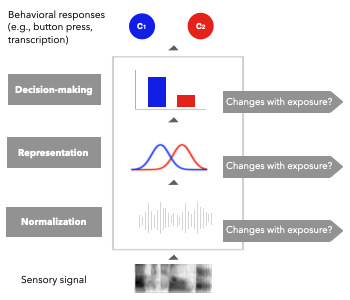
\includegraphics[width=0.6\columnwidth]{../figures/diagrams/overview-of-three-mechanisms2.png}
\caption{Listeners' recognition of speech categories are typically assumed to involve at least three types of mechanisms: 1) the acoustic input is transformed by low-level normalization processes into the perceptual cues that form the input to categorization, 2) linguistic representations describe the mapping between these perceptual and linguistic categories, and 3) decision-making mechanisms allow additional, stimulus-independent, biases to affect recognition. Any of these three mechanisms can in theory be affected by recent experience. While it is now clear \emph{that} recent experience changes the processing of subsequent speech input, most existing findings leave open \emph{which of the three mechanisms underlie these changes.}}\label{fig:overview}
\end{center}
\end{figure}

The majority of recent research on talker-related adaptation has focused on the middle layer, changes in linguistic representations. This includes proposals that attribute exposure effects to ``boundary re-tuning/shifts'' (e.g., \protect\hyperlink{ref-norris2003}{Norris, McQueen, \& Cutler, 2003}; \protect\hyperlink{ref-reinisch2011}{Reinisch, Weber, \& Mitterer, 2011}), ``perceptual/category recalibration'' (e.g., \protect\hyperlink{ref-kraljic-samuel2006}{Kraljic \& Samuel, 2006}; \protect\hyperlink{ref-reinisch-holt2014}{Reinisch \& Holt, 2014}; \protect\hyperlink{ref-samuel2016}{Samuel, 2016}; \protect\hyperlink{ref-vroomen-baart2009}{Vroomen \& Baart, 2009}), ``perceptual retuning'' (\protect\hyperlink{ref-jesse-mcqueen2011}{Jesse \& McQueen, 2011}; \protect\hyperlink{ref-mcqueen2006}{McQueen, Cutler, \& Norris, 2006}; \protect\hyperlink{ref-mitterer2013}{Mitterer, Scharenborg, \& McQueen, 2013}), ``category expansion'' (\protect\hyperlink{ref-schmale2012}{Schmale, Cristia, \& Seidl, 2012}), ``dimension-based statistical learning'' (\protect\hyperlink{ref-idemaru-holt2011}{Idemaru \& Holt, 2011}; \protect\hyperlink{ref-lehet-holt2020}{Lehet \& Holt, 2020}; \protect\hyperlink{ref-liu-holt2015}{R. Liu \& Holt, 2015}), or ``criteria relaxation'' (\protect\hyperlink{ref-zheng-samuel2020}{Zheng \& Samuel, 2020}). While these proposals are often not further formally specified {[}or modeled; for notable exceptions, see Apfelbaum and McMurray (\protect\hyperlink{ref-apfelbaum-mcmurray2015}{2015}); Clayards et al. (\protect\hyperlink{ref-clayards2008}{2008}); Hitczenko and Feldman (\protect\hyperlink{ref-hitczenko-feldman2016}{2016}); Kleinschmidt and Jaeger (\protect\hyperlink{ref-kleinschmidt-jaeger2015}{2015}); Lancia and Winter (\protect\hyperlink{ref-lancia-winter2013}{2013}); Theodore and Monto (\protect\hyperlink{ref-theodore-monto2019}{2019}); X. Xie, Buxó-Lugo, et al. (\protect\hyperlink{ref-xie2021cognition}{2021}){]}, all of them seem to describe types of changes in representations. For example, ``category shift'' refers to a change in the mean of the cue distribution corresponding to a category, and ``category expansion'' refers to increases in the variance of that distribution. Either of these changes, along with ``cue re-weighting'' or ``learning of new cues'', can be understood as a consequence of the type of distributional learning that is hypothesized in exemplar (\protect\hyperlink{ref-apfelbaum-mcmurray2015}{Apfelbaum \& McMurray, 2015}; \protect\hyperlink{ref-johnson2006}{Johnson, 2006}), episodic (\protect\hyperlink{ref-goldinger1998}{Goldinger, 1998}), Bayesian inference (\protect\hyperlink{ref-kleinschmidt-jaeger2015}{Kleinschmidt \& Jaeger, 2015}), or neural network models (\protect\hyperlink{ref-lancia-winter2013}{Lancia \& Winter, 2013}). Indeed, recent reviews discuss \emph{what types} of representational changes underlie the effects of recent exposure (e.g., ``category expansion'' vs.~``category shifts''), rather than \emph{whether} representational changes are the actual mechanism underlying the observed results (e.g., \protect\hyperlink{ref-baeseberk2020}{Baese-Berk et al., 2020}; \protect\hyperlink{ref-bent-baeseberk2021}{Bent \& Baese-Berk, 2021}; \protect\hyperlink{ref-schertz-clare2020}{Schertz \& Clare, 2020}). In our own work, we have sometimes made similar assumptions---e.g., when asking whether representational changes can account for adaptation without considering alternative explanations (\protect\hyperlink{ref-kleinschmidt-jaeger2011}{Kleinschmidt \& Jaeger, 2011}, \protect\hyperlink{ref-kleinschmidt-jaeger2012}{2012}, \protect\hyperlink{ref-kleinschmidt-jaeger2016cogsci}{2016b}; \protect\hyperlink{ref-kurumada2017}{Kurumada, Brown, \& Tanenhaus, 2017}; \protect\hyperlink{ref-tan2021}{Tan, Xie, \& Jaeger, 2021}).

An absence of contrastive tests, however, means that the same behavioral results could in principle be explained by an alternative mechanism that assumes \emph{no change of linguistic representations}. For instance, if is possible that adaptive changes of responses can be due to low-level, automatic (involuntary) normalization during the early stages of auditory processing (bottom of Figure \ref{fig:overview}) These processes are thought to be pre-linguistic in that they do not refer to categories but rather apply to the acoustic or phonetic cues (\protect\hyperlink{ref-johnson-sjerps2021}{Johnson \& Sjerps, 2021}; \protect\hyperlink{ref-stilp2020}{Stilp, 2020}). In contrast to the assumption that cross-talker variability may be learned and stored, which is fundamental to all the theories of representational changes as described above, theories in normalization assume that listeners remove (or discard) talker variability prior to mapping cues to linguistic categories. \emph{That} such processes help navigate cross-talker variability is widely assumed both in behavioral and neuroimaging research (\protect\hyperlink{ref-irino-patterson2014}{Irino \& Patterson, 2014}; \protect\hyperlink{ref-johnson1990}{Johnson, 1990}; e.g., \protect\hyperlink{ref-kluender1988}{Kluender et al., 1988}; \protect\hyperlink{ref-newman-sawusch1996}{Newman \& Sawusch, 1996}; \protect\hyperlink{ref-pisoni1977}{Pisoni, 1977}; \protect\hyperlink{ref-sawusch-newman2000}{Sawusch \& Newman, 2000}; \protect\hyperlink{ref-sjerps2011}{Sjerps et al., 2011a}; \protect\hyperlink{ref-uddin2020}{Uddin, Reis, Heald, Hedger, \& Nusbaum, 2020}; for discussion, see \protect\hyperlink{ref-barreda2012}{Barreda, 2012}; \protect\hyperlink{ref-magnuson-nusbaum2007}{Magnuson \& Nusbaum, 2007}; \protect\hyperlink{ref-wong2004}{Wong et al., 2004}). However, distinct normalization procedures have mostly been compared to each other (e.g., \protect\hyperlink{ref-adank2004}{Adank, Smits, \& Hout, 2004}; \protect\hyperlink{ref-hoffmanbion-escudero2007}{Hoffmann Bion \& Escudero, 2007}; \protect\hyperlink{ref-kiefte-nearey2019}{Kiefte \& Nearey, 2019}) or against the absence of normalization (\protect\hyperlink{ref-mcmurray-jongman2011}{McMurray \& Jongman, 2011}). They are often not considered as a competing explanation when researchers interpret the results of experiments on accent adaptation, perceptual recalibration, or distributional learning (but see \protect\hyperlink{ref-mullennix-pisoni1990}{Mullennix \& Pisoni, 1990}; \protect\hyperlink{ref-sjerps-reinisch2015}{Sjerps \& Reinisch, 2015}). Only a handful of recent studies have begun to do so for specific contrast types. With some (e.g., English fricatives (\protect\hyperlink{ref-chodroff-wilson2020}{Chodroff \& Wilson, 2020})), low-level auditory normalization has been found to explain human perception of fricatives better than changes in representations.

Yet alternatively, it is possible that \emph{post-linguistic} mechanisms underlie the effects of recent exposure (top of Figure \ref{fig:overview}). Just like normalization is broadly accepted to be part of speech perception, there is little doubt that changes in response biases can affect listeners' interpretation of speech input, or at least the responses they give within experiments. For instance, Clarke-Davidson et al. (\protect\hyperlink{ref-clarkedavidson2008}{2008, p. 605}) define a bias as ``the increased likelihood to give a particular response---such as /s/---given any acoustic input, or the need for less evidence for a particular response'' that ``would help participants make faster word decisions in {[}\ldots{]} ambiguous cases''. However, such biases are rarely considered in the behavioral literature when analyzing the effects of recent exposure. \emph{When} response biases have been considered (e.g., as ``response equilibration'' in Vroomen and Baart \protect\hyperlink{ref-vroomen-baart2009}{2009}), this explanation tends to be dismissed---prematurely, we believe. One reason for this might be particular result patterns---such as boundary shifts in perceptual recalibration or improved categorization or transcription accuracy in accent adaptation---are considered unlikely to be explained by changes in response biases (or normalization, for that matter).

In investigations into neural systems, in contrast, it is commonplace to isolate prefrontal areas (e.g., \protect\hyperlink{ref-binder2004neural}{Binder, Liebenthal, Possing, Medler, \& Ward, 2004}; \protect\hyperlink{ref-thompson1997role}{Thompson-Schill, D'Esposito, Aguirre, \& Farah, 1997}) as well as the insula and parietal cortex (e.g., \protect\hyperlink{ref-furl2011parietal}{Furl \& Averbeck, 2011}; \protect\hyperlink{ref-keuken2014}{Keuken et al., 2014}) as responsible for perceptual decision-making. Recent studies have begun to investigate whether adaptive changes in speech perception primarily recruit these areas (\protect\hyperlink{ref-erb2013brain}{Erb, Henry, Eisner, \& Obleser, 2013}; \protect\hyperlink{ref-myers-mesite2014}{Myers \& Mesite, 2014}) as opposed to cortical areas associated with phonetic representations (\protect\hyperlink{ref-bonte2017}{Bonte, Correia, Keetels, Vroomen, \& Formisano, 2017}; \protect\hyperlink{ref-luthra2020}{\textbf{luthra2020?}}). For instance, Myers and Mesite (\protect\hyperlink{ref-myers-mesite2014}{2014}) have suggested that sensitivity to boundary shifts between {[}s{]} and {[}\ipatext{ʃ}{]} emerged in right frontal and middle temporal regions, implicating adjustments of decision-related or attentional criteria downstream from primary auditory cortex. Similarly, a recent work on adaptation to phoneme category substitutions (e.g., {[}s{]} pronounced as {[}\ipatext{ʃ}{]}) found evidence that adaptive processing of such phoneme substitutions engages prefrontal regions, responsible for post-perceptual \emph{repair} mechanisms (\protect\hyperlink{ref-blanco-elorriera2021}{Blanco-Elorrieta, Gwilliams, Marantz, \& Pylkkänen, 2021}): simply put, listeners seemed to initially map the acoustic input onto the wrong category and subsequently corrects the mapping. This was contrasted with the hypothesis that adaptation occurs via returning of the lower level functional connections (e.g., between STG and primary auditory cortex).\footnote{We note that other lines of imaging research have focused on pre-linguistic signal transformations (\protect\hyperlink{ref-sjerps2011listening}{Sjerps, Mitterer, \& McQueen, 2011b}; \protect\hyperlink{ref-zhang2016functionally}{C. Zhang et al., 2016}) and sensory adaptation (\protect\hyperlink{ref-guediche2015evidence}{Guediche et al., 2015}), including sub-cortical structures (e.g., the brain stem, \protect\hyperlink{ref-skoe2021auditory}{Skoe, Krizman, Spitzer, \& Kraus, 2021}; and cerebellum, \protect\hyperlink{ref-guediche2014}{Guediche, Blumstein, Fiez, \& Holt, 2014}). Compared to the behavioral research we reviewed, it is more common to directly contrast hypotheses that are associated with functionally distinct areas and networks. Like the behavioral research, however, no study to date has examined the three mechanisms in a coherent framework. Studies often adopt stimuli and experimental design that are strongly constrained by particular hypotheses researchers intend to test. The recommendations we provide in General Discussion will help facilitate direct tests across multiple mechanisms.}

Across the behavioral and neuroimaging work, the past research has thus split the underlying process of speech perception (Figure \ref{fig:overview}) in distinct ways. Behavioral studies have begun to distinguish between the (A) normalization and (B) representational changes while continuing to treat (C) post-perceptual decision-making as a factor external to perception. In contrast, the neuroimaging work tends to group (A) and (B) together as happening early in the neural processing stream, functionally distinct from (C) i.e., higher-level, decision-related mechanisms further downstream. To meaningfully link these lines of work, and to better elucidate how human speech perception operates over the variable acoustic input, we need a framework that can encompass (A)-(C) (for a related discussion, see \protect\hyperlink{ref-guediche2014}{Guediche et al., 2014, p. 8}). More specifically, we need a framework to formalize and implement the competing hypotheses about the effects of recent exposure on subsequent speech perception. By testing these predictions using a coherent experimental design, we will be able to test if any of the mechanisms (A)-(C), and \emph{only} that mechanism, can account for adaptive changes seen in human responses.

This motivates the present study. Our long-term goal is to contribute to the development of stronger theories that make specific predictions, facilitating more decisive tests (cf. \protect\hyperlink{ref-platt1964}{Platt, 1964}). As a first step, here we develop a general, unified framework that implements the three distinct theories of adaptive speech perception (i.e., (A)-(C) in Figure \ref{fig:overview}). To anticipate our results, our simulations will demonstrate that the vast majority of existing results do \emph{not} distinguish between three different explanations. We will show this in two highly influential paradigms: so-called \textbf{perceptual recalibration} (e.g., \protect\hyperlink{ref-kraljic-samuel2006}{Kraljic \& Samuel, 2006}; \protect\hyperlink{ref-reinisch-holt2014}{Reinisch \& Holt, 2014}; \protect\hyperlink{ref-samuel2016}{Samuel, 2016}; \protect\hyperlink{ref-vroomen-baart2009}{Vroomen \& Baart, 2009}) and \textbf{(foreign) accent adaptation} (e.g., \protect\hyperlink{ref-bradlow-bent2008}{Bradlow \& Bent, 2008}; \protect\hyperlink{ref-hernandez2019}{Hernández, Ventura-Campos, Costa, Miró-Padilla, \& Ávila, 2019}; \protect\hyperlink{ref-sidaras2009}{Sidaras et al., 2009}; \protect\hyperlink{ref-tzeng2016}{Tzeng, Alexander, Sidaras, \& Nygaard, 2016}; \protect\hyperlink{ref-xie2016jep}{X. Xie, Theodore, \& Myers, 2016}; \protect\hyperlink{ref-zheng-samuel2020}{Zheng \& Samuel, 2020}). In each, result patterns taken as signature evidence of one mechanism (e.g., changes of representations) could be predicted by \emph{any of the three mechanisms}. To us, and we expect to others in the field, the degree to which this is the case was surprising. These separate lines of research (our own work included) seem to have drawn theoretical conclusions through convention, rather than through strong empirical evidence in favor of a particular mechanism.

As we discussed above, the assumption that our \emph{linguistic representations} adapt to recent exposure has been central to recent breakthroughs in speech perception research (e.g., \protect\hyperlink{ref-hay2019}{Hay, Walker, Sanchez, \& Thompson, 2019}; \protect\hyperlink{ref-kleinschmidt-jaeger2015}{Kleinschmidt \& Jaeger, 2015}; \protect\hyperlink{ref-luthra2020a}{Luthra, Correia, Kleinschmidt, Mesite, \& Myers, 2020}; \protect\hyperlink{ref-sjerps2019}{Sjerps, Fox, Johnson, \& Chang, 2019}). Evidence supporting this assumption has helped shape linguistic theories (\protect\hyperlink{ref-baeseberk2013}{Baese-Berk, Bradlow, \& Wright, 2013}; e.g., \protect\hyperlink{ref-bradlow-bent2008}{Bradlow \& Bent, 2008}; \protect\hyperlink{ref-goldinger-azuma2004}{Goldinger \& Azuma, 2004}; \protect\hyperlink{ref-hay2019}{Hay et al., 2019}; \protect\hyperlink{ref-magnuson-nusbaum2007}{Magnuson \& Nusbaum, 2007}; \protect\hyperlink{ref-tzeng2016}{Tzeng et al., 2016}) as well as theories about the interface between social and linguistic cognition (e.g., \protect\hyperlink{ref-babel2019}{Babel, Senior, \& Bishop, 2019}; \protect\hyperlink{ref-creel-bregman2011}{Creel \& Bregman, 2011}; \protect\hyperlink{ref-foulkes-hay2015}{Foulkes \& Hay, 2015}; \protect\hyperlink{ref-hanulikova2012}{Hanulíková, Alphen, Goch, \& Weber, 2012}; \protect\hyperlink{ref-sumner2014}{Sumner, Kim, King, \& McGowan, 2014}). The empirical indeterminacy that we present calls for a scrutiny of this assumption. Even if one were to take for granted that the three mechanisms in Figure \ref{fig:overview} \emph{jointly} underlie the effects of recent exposure, it remains unclear which of those mechanisms any given results sheds light on. For example, can we conclude from experiments like Clarke and Garrett (\protect\hyperlink{ref-clarke-garrett2004}{2004}) that listeners can learn new representations (or at least select some mixture of existing representations) within two minutes of exposure? Or are those results due to normalization, making them substantially less thought-provoking? Also, do the results of perceptual recalibration and accent adaptation stem from the same mechanism(s), or do they reflect different mechanisms (\protect\hyperlink{ref-baeseberk2018}{Baese-Berk, Walker, \& Bradlow, 2018}; \protect\hyperlink{ref-samuel-kraljic2009}{Samuel \& Kraljic, 2009}; \protect\hyperlink{ref-zheng-samuel2020}{Zheng \& Samuel, 2020})? Our comprehensive framework will make it possible to empirically test whether two paradigms that differ substantially in their design, tasks, and ecological validity of the speech stimuli would in fact engage the same mechanism(s).

\begin{figure}[h]
\begin{center}
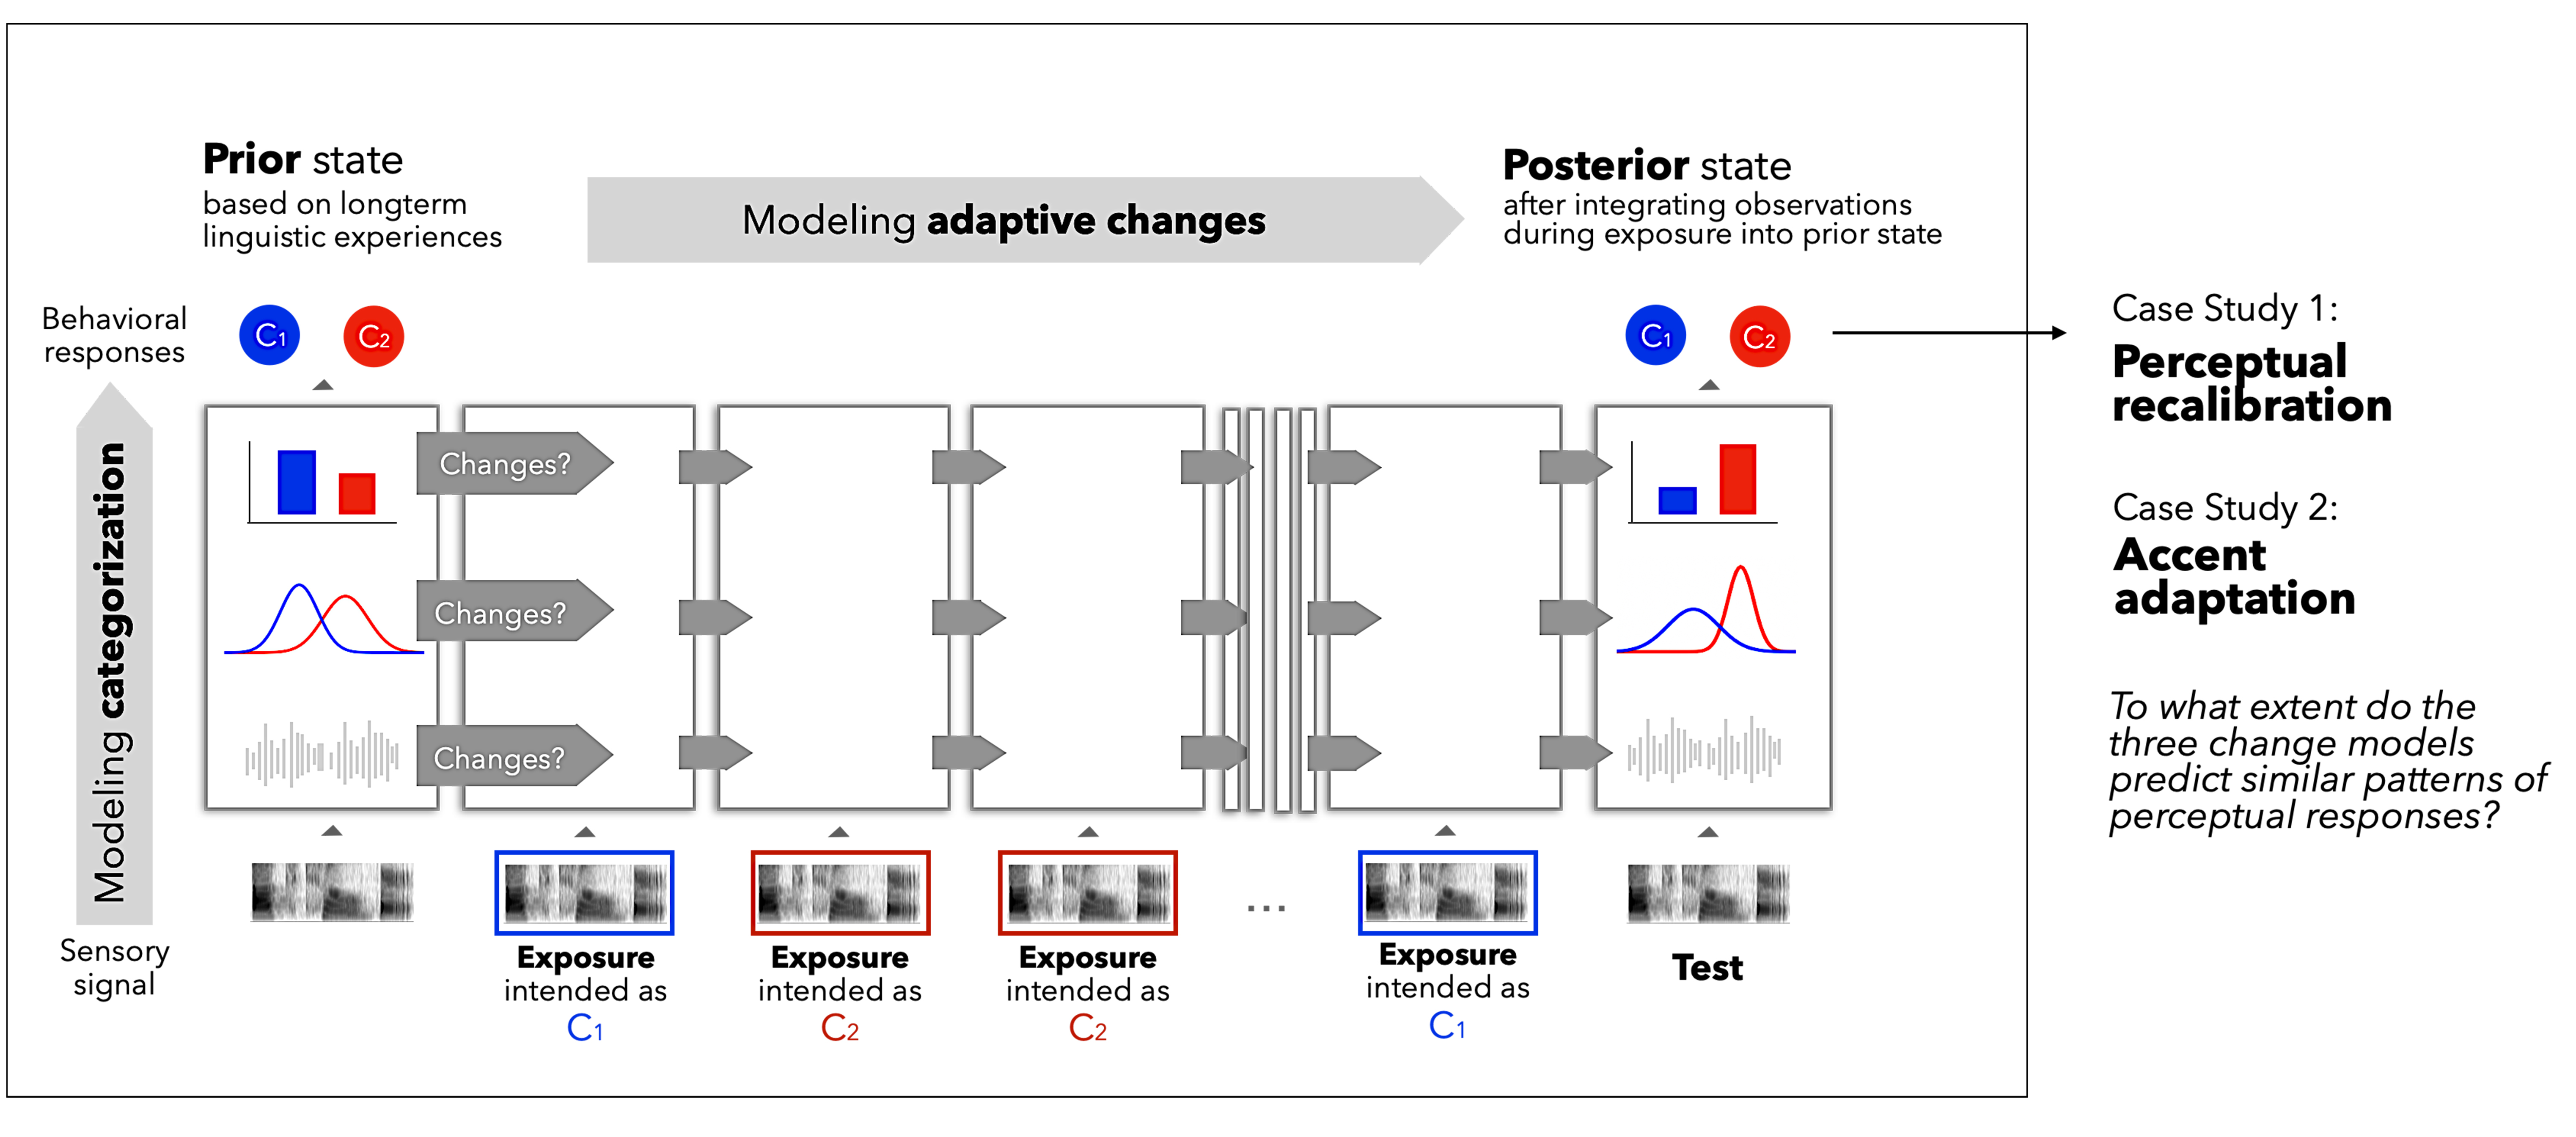
\includegraphics[width=.99\columnwidth]{../figures/diagrams/overview-of-changes.png}
\caption{Overview of our approach. Experiments on the effect of recent exposure on subsequent speech perception tend to involve two phases. An exposure phase manipulates the statistics of speech input between participants. A subsequent test phase assesses the effects of those manipulations on the interpretation of identical speech input. We seek to understand what type of exposure effects each of the three three mechanisms in Figure \ref{fig:overview} can explain. To this end, we specify both a) a {\em categorization model} that describes the interpretation of speech input at any given moment (vertical information flow) and b) {\em change models} for all three mechanism that describe how these parts of the categorization model change as a function of exposure (horizontal information flow). We then use the different change models to compare the predicted consequences of changes to normalization, representations, or response biases.}\label{fig:overview-change}
\end{center}
\end{figure}

The approach we take in this article is illustrated in Figure \ref{fig:overview-change}. We extend the three-pronged process of speech perception (Figure \ref{fig:overview}) to implement \emph{change models} describing how normalization, representations, and responses biases may change with exposure. By training these change models on large-scale production corpora, we simulate adaptive changes of human responses predicted under a given hypothesized mechanism. Our main finding is two fold. First, as we stated above, existing data do not decisively separate their predictions. Present-day conventions in experimental design and analysis severely limit the discriminatory power of behavioral results over the underlying mechanisms. Second, perhaps more significant, it \emph{will} be possible to distinguish the mechanisms from one another if new standards are applied for selection of adaptor/test stimuli as well as for statistical tests. Results of our simulations illuminate when---to what stimuli and under what circumstances---the three mechanisms would provide diverging predictions about adaptive changes of perception. We also learn about how much data will be needed to draw reliable statistical inferences from behavioral data. The general discussion will elaborate on these new standards and how they can be achieved.

All data and code for this article can be downloaded from OSF at \url{https://osf.io/q7gjp/}. This article is written in R markdown, allowing readers to replicate our analyses with the press of a button using freely available software (R, \protect\hyperlink{ref-R}{R Core Team, 2021a}; \protect\hyperlink{ref-RStudio}{RStudio Team, 2020}), while changing any of the parameters of our models. Readers can revisit any of the assumptions we make---for example, by substituting alternative models of linguistic representations. The supplementary information (SI, \ref{sec:SI-software}) lists the software/libraries required to compile this document. Beyond our immediate goals here, we hope that this can be helpful to researchers who are interested in developing more informative experimental designs, and to facilitate the interpretation of existing results (see also \protect\hyperlink{ref-tan2021}{Tan et al., 2021}).

\hypertarget{sec:framework}{%
\section{Modeling adaptive changes in speech perception}\label{sec:framework}}

We start by describing the computational framework. Our goal here is not to present a new model of speech perception but rather to describe a framework that i) integrates the core insights shared by present-day theories of speech perception, ii) extends these models to specify ways to think about how recent exposure can come to affect any of the three mechanistic levels, and iii) stays as simple and conceptually transparent as possible. The framework builds on a psychometric model that is used for data analysis in many areas of the cognitive sciences (for an introduction, see \protect\hyperlink{ref-wichmann-hill2001}{Wichmann \& Hill, 2001}) but remains rare in research on speech perception---in particular, in research on the effects of recent experience (but see \protect\hyperlink{ref-clayards2008}{Clayards et al., 2008}; \protect\hyperlink{ref-kleinschmidt-jaeger2016cogsci}{Kleinschmidt \& Jaeger, 2016b}). We extend this psychometric model in as few ways as necessary. Most notably, this includes the specification of competing linking hypotheses that describe the effects of recent exposure on normalization, representations, and/or response biases.

We assume conceptual familiarity with reasoning about distributions and contemporary theories of speech perception---all of which expect that listeners have implicit representations of the mapping between phonetic cues and linguistic categories that encompass (in one form or other) knowledge of the distribution of cues that correspond to a linguistic category. This logic is motivated by observations such as shown in Figure \ref{fig:schertzclare} (reprinted from \protect\hyperlink{ref-schertz-clare2020}{Schertz \& Clare, 2020}): human listeners' perceptual judgments on two phonetic categories /b/ and /p/ (Figure \ref{fig:schertzclare}B) can be predicted by considering the phonetic properties of the input \emph{relative to the distribution of phonetic cues} that listeners have previously experienced (Figure \ref{fig:schertzclare}A). For recent, introductions to distributional thinking about the production-perception link, we refer to Bent and Baese-Berk (\protect\hyperlink{ref-bent-baeseberk2021}{2021}), Kurumada and Roettger (\protect\hyperlink{ref-kurumada-roettger2021}{2021}), Quam and Creel (\protect\hyperlink{ref-quam-creel2021}{2021}), and Schertz and Clare (\protect\hyperlink{ref-schertz-clare2020}{2020}).

\begin{figure}[h]
\begin{center}
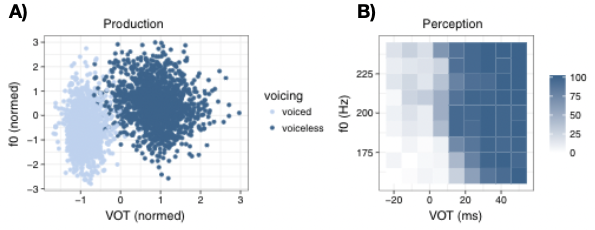
\includegraphics[width=.7\columnwidth]{../figures/diagrams/schertzclare.png}
\caption{Speech production realizes phonetic categories as distributions in a multi-dimensional acoustic or phonetic cue space. Implicit knowledge of these distributions is known to mediate listeners’ interpretation of speech inputs (reprinted from Schertz and Clare, 2020, permission pending). {\bf Panel A:} voice onset time (VOT) and fundemental frequency (f0) of word-initial stops from 24 English speakers' productions (data from Schertz, 2014). {\bf Panel B:} 24 English listeners' responses to a 2AFC ``ba'' vs. ``pa'' categorization task depending on VOT and f0. Each cell represents one stimulus, with the shading of the cell representing the percentage of ``pa'' response (data from Schertz, Cho, Lotto, and Warner, 2016).}\label{fig:schertzclare}
\end{center}
\end{figure}

We focus on modeling offline responses, which remain one of the most commonly employed measures in research on speech perception. This includes categorization/identification responses in two-forced-choice (2AFC) tasks that continue to be the standard approach to assessing the effects of recent exposure on subsequent speech perception. 2AFC tasks are used in the test phases of experiments on perceptual recalibration (\protect\hyperlink{ref-drouin2016}{Drouin, Theodore, \& Myers, 2016}; \protect\hyperlink{ref-kraljic-samuel2006}{Kraljic \& Samuel, 2006}; \protect\hyperlink{ref-liu-jaeger2018}{L. Liu \& Jaeger, 2018}; e.g., \protect\hyperlink{ref-norris2003}{Norris et al., 2003}; \protect\hyperlink{ref-reinisch-holt2014}{Reinisch \& Holt, 2014}; \protect\hyperlink{ref-vroomen2007}{Vroomen, Linden, Gelder, \& Bertelson, 2007}; \protect\hyperlink{ref-zheng-samuel2020}{Zheng \& Samuel, 2020}) and distributional learning (e.g., \protect\hyperlink{ref-clayards2008}{Clayards et al., 2008}; \protect\hyperlink{ref-kleinschmidt2015}{Kleinschmidt, Raizada, \& Jaeger, 2015}; \protect\hyperlink{ref-maye2008}{Maye et al., 2008}; \protect\hyperlink{ref-munson2011}{Munson, 2011}), and are also used in experiments on accent adaptation (e.g., \protect\hyperlink{ref-xie2017}{X. Xie \& Myers, 2017}). The same general framework we develop here can, however, be extended to offline and online tasks with two or more categorical outcomes, including spoken repetition (e.g., \protect\hyperlink{ref-bieber2021}{Bieber \& Gordon-Salant, 2021}), transcription (e.g., \protect\hyperlink{ref-bradlow-bent2008}{Bradlow \& Bent, 2008}; \protect\hyperlink{ref-clopper-bradlow2008}{Clopper \& Bradlow, 2008}; \protect\hyperlink{ref-cooper-bradlow2016}{Cooper \& Bradlow, 2016}; \protect\hyperlink{ref-gordonsalant2010}{Gordon-Salant, Yeni-Komshian, Fitzgibbons, \& Schurman, 2010}), accuracy in cross-modal priming (\protect\hyperlink{ref-clarke-garrett2004}{Clarke \& Garrett, 2004}; e.g., \protect\hyperlink{ref-eisner2013}{Eisner, Melinger, \& Weber, 2013}; \protect\hyperlink{ref-sjerps-mcqueen2010}{Sjerps \& McQueen, 2010}; \protect\hyperlink{ref-xie2018jasa}{X. Xie, Weatherholtz, et al., 2018}), or fixations in the visual world paradigm (e.g., \protect\hyperlink{ref-hanulikova-weber2012}{Hanulíková \& Weber, 2012}; \protect\hyperlink{ref-nixon2016}{Nixon, Rij, Mok, Baayen, \& Chen, 2016}). It is also conceptually related to general process models of online perceptual decision-making (e.g., the drift diffusion model, \protect\hyperlink{ref-ratcliff2011}{Ratcliff, Hugenberg, Shriver, \& Bernstein, 2011}). \footnote{We also note that here we focus on the recognition of phonetic categories---be it a phoneme, syllable, or word--- \emph{out of context}. We do not aim to model the well-documented effects of phonotactic (e.g., \protect\hyperlink{ref-carlisle1991}{Carlisle, 1991}; \protect\hyperlink{ref-cutler-jesse2021}{Cutler \& Jesse, 2021}), prosodic (e.g., \protect\hyperlink{ref-munro1995}{Munro, 1995}; \protect\hyperlink{ref-sereno2015}{Sereno, Lammers, \& Jongman, 2015}), lexical/semantic (e.g., \protect\hyperlink{ref-cooper-bradlow2016}{Cooper \& Bradlow, 2016}; \protect\hyperlink{ref-davis2005}{Davis et al., 2005}), visual (e.g., \protect\hyperlink{ref-bertelson2003}{Bertelson, Vroomen, \& Gelder, 2003}; \protect\hyperlink{ref-ganong1980}{Ganong, 1980}; \protect\hyperlink{ref-vroomen-baart2009}{Vroomen \& Baart, 2009}; \protect\hyperlink{ref-vroomen2007}{Vroomen et al., 2007}) and sentential/discourse context (e.g., \protect\hyperlink{ref-contemori-tortajada2020}{Contemori \& Tortajada, 2020}; \protect\hyperlink{ref-holt-bent2017}{R. F. Holt \& Bent, 2017}; \protect\hyperlink{ref-klatt1975}{Klatt, 1975}; \protect\hyperlink{ref-winn2018}{Winn, 2018}). The results we present below generalize to situations in which such context is taken into account (in the formulation of our model, context simply changes the overall response bias). Critically, some models of spoken word recognition have been shown to capture contextual effects (DIANA, \protect\hyperlink{ref-bosch2015}{Bosch, Boves, Tucker, \& Ernestus, 2015}; NAM, \protect\hyperlink{ref-luce-pisoni1998}{P. A. Luce \& Pisoni, 1998}; TRACE, \protect\hyperlink{ref-mcclelland-elman1986}{McClelland \& Elman, 1986}; EARSHOT, \protect\hyperlink{ref-magnuson2020}{Magnuson et al., 2020}), and these models share the general assumptions we make here.}

For the present purpose, we can think of the the mapping from acoustic inputs to categorization responses as involving three sets of processes illustrated in Figure \ref{fig:model-perceptual-decision-making}.
We first describe these three mechanistic levels along with the parameters they introduce (\(\lambda\), \(\pi\)s, \(\mu_c\)s, \(\Sigma_c\)s, and \(\mu\) in Figure \ref{fig:model-perceptual-decision-making}). Then we introduce the linking hypotheses that describe how the parameters that characterize each mechanism can change with exposure.

\begin{figure}[h]
\begin{center}
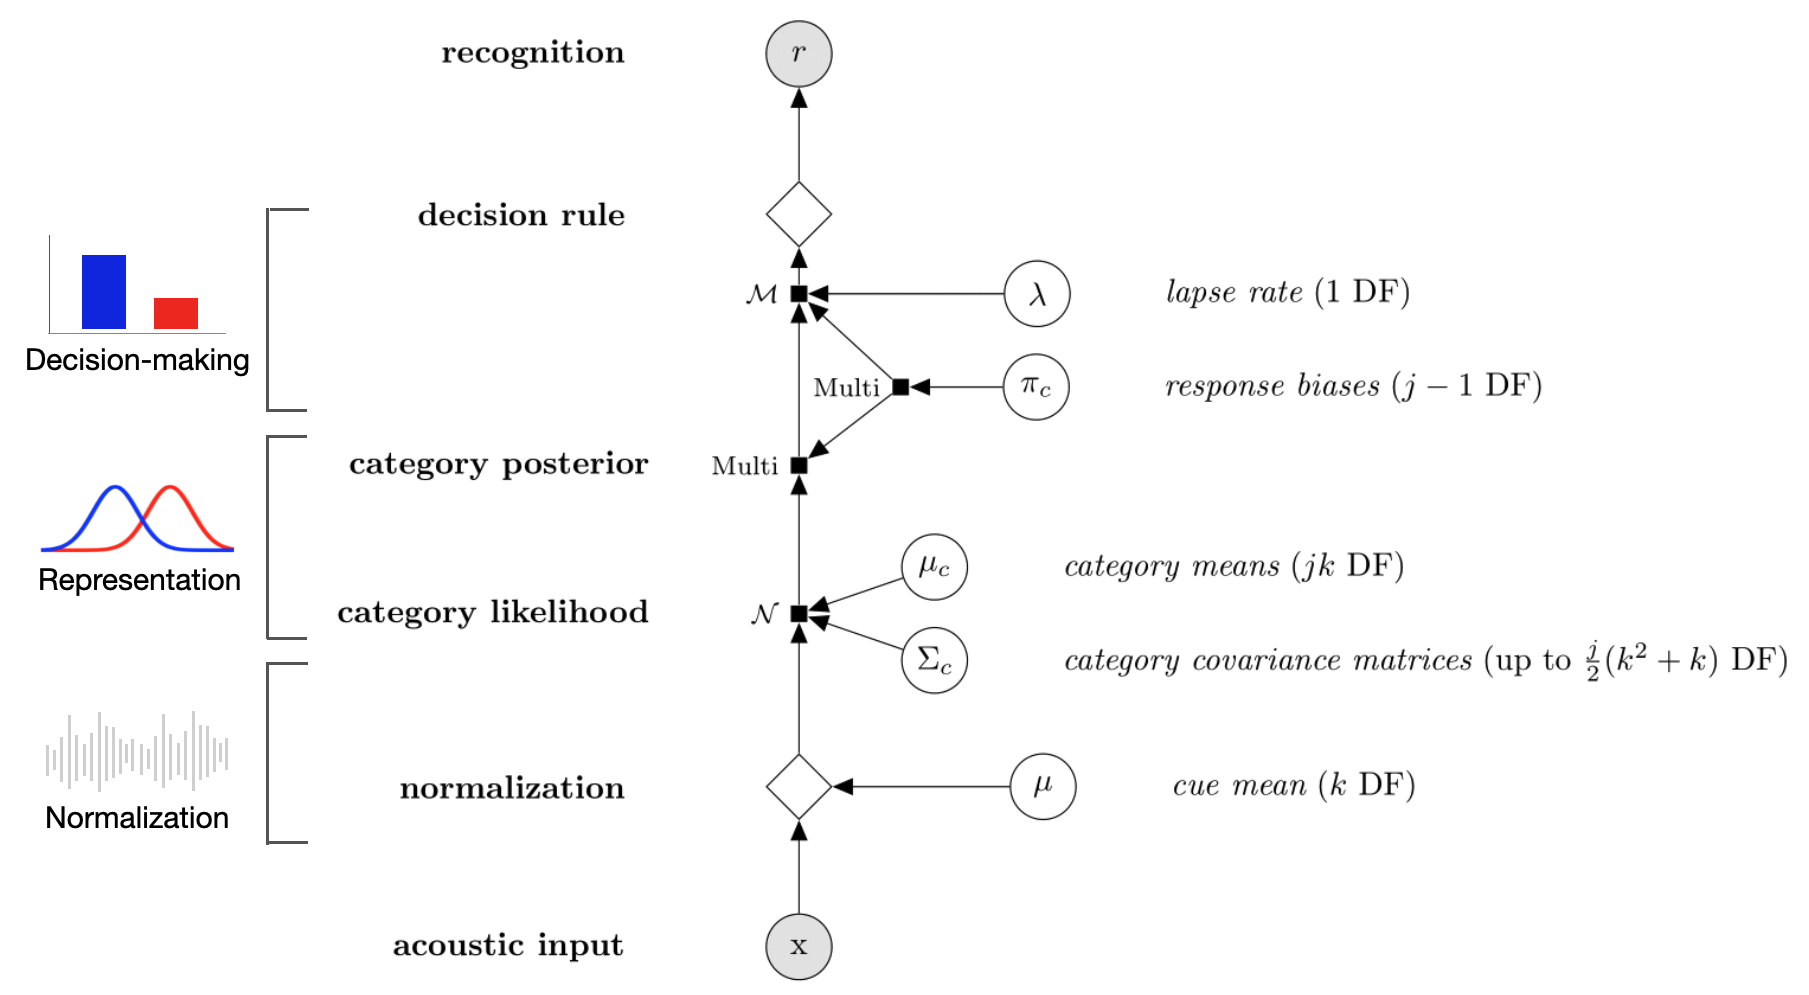
\includegraphics[width=.9\columnwidth]{../figures/diagrams/graphical-model.png}
  \caption{A simplified general {\em categorization model} for $J$-AFC alternative-choice tasks (e.g., vowel categorization, word transcription, etc.) over a $K$-dimensional phonetic input. Filled gray circles represent variables the researcher can observe. Empty circles represent latent variables that are not observable. Diamonds represent variable-free processes. Only variables that we consider as being potentially affected by recent exposure are shown (see text for additional detail). Parentheses describe the number of degrees of freedom (DF) introduced by each parameter. In practice, many of these DFs can be fixed based on phonetic databases and/or previous perception experiments (see text for details). Squares are annotated with the distributions resulting at that level of the model: $\mathcal{N}$(ormal), Multi(nomial), and $\mathcal{M}$(ixture) distributions. For 2AFC tasks, all multinomial distributions simplify to Bin(omial) distributions.} \label{fig:model-perceptual-decision-making}
\end{center}
\end{figure}

\hypertarget{pre-linguistic-processes-signal-transformations-and-normalization}{%
\subsection{`Pre-linguistic' processes: signal transformations and normalization}\label{pre-linguistic-processes-signal-transformations-and-normalization}}

The first step in our categorization model maps the acoustic input onto \emph{perceptual} features. These perceptual features are the outcome of low-level signal transformations and normalization processes.\footnote{The term normalization is often used to refer to both of these components together. For example, some of the most common normalization approaches involve both log-transforms and further normalization steps (e.g., Lobanov normalization, \protect\hyperlink{ref-lobanov1971}{Lobanov, 1971}; height-backness normalization, \protect\hyperlink{ref-miller1989}{Miller \& Volaitis, 1989}). Transformation and normalization can, however, be understood as separate processes (see also ``vowel-intrinsic'' vs.~``vowel-extrinsic'' procedures in \protect\hyperlink{ref-adank2004}{Adank et al., 2004}).} Experiments on the perception of stimulus similarity suggest, for example, that the human brain represents frequency information logarithmically (\protect\hyperlink{ref-greenwood1961}{Greenwood, 1961}). This is captured by, for example, the Mel (\protect\hyperlink{ref-stevens1937}{Stevens, Volkmann, \& Newman, 1937}), Bark (\protect\hyperlink{ref-zwicker1961}{Zwicker, 1961}), and ERB (\protect\hyperlink{ref-moore-glasberg1983}{Moore \& Glasberg, 1983}) transformations. Such logarithm-transformed spectral cues have been found to provide a better fit against human categorization responses than features based on raw frequencies (\protect\hyperlink{ref-hoffmanbion-escudero2007}{Hoffmann Bion \& Escudero, 2007}; \protect\hyperlink{ref-kleinschmidt2019}{Kleinschmidt, 2019}; \protect\hyperlink{ref-richter2017}{Richter, Feldman, Salgado, \& Jansen, 2017}). The case studies we present below model perception for a phonological contrast that depends on both temporal and spectral cues. For the spectral cue, we use Mel-transformed frequencies.

\emph{Normalization} refers to further transformation of acoustic inputs based on either other acoustic properties or the overall distribution of the acoustic input itself (for a review, see \protect\hyperlink{ref-weatherholtz-jaeger2016}{Weatherholtz \& Jaeger, 2016}). For example, one of the most influential normalization procedures for the formant cues that affect vowel perception centers and standardizes these cues based on the talker-specific mean and standard deviation of the formant values (\protect\hyperlink{ref-lobanov1971}{Lobanov, 1971}). This and conceptually similar normalizations (e.g., \protect\hyperlink{ref-gerstman1968}{Gerstman, 1968}) have been found to remove a substantial amount of cross-talker variability in the realization in vowels while maintaining phonemic contrasts and sociolinguistic information (\protect\hyperlink{ref-adank2004}{Adank et al., 2004}), providing a good fit against vowel categorization by human listeners (\protect\hyperlink{ref-hoffmanbion-escudero2007}{Hoffmann Bion \& Escudero, 2007}). Because normalization operates prior to linguistic representations, it potentially provides a particularly efficient way to remove uninformative variability---e.g., by taking advantage of \emph{all} available information about a cue, not just the observations of a specific set of categories (\protect\hyperlink{ref-apfelbaum-mcmurray2015}{Apfelbaum \& McMurray, 2015}).

The case studies we present below employ a general model of normalization that can be applied to any type of phonological contrast (C-CuRE, \protect\hyperlink{ref-cole2010}{Cole, Linebaugh, Munson, \& McMurray, 2010}; \protect\hyperlink{ref-mcmurray-jongman2011}{McMurray \& Jongman, 2011}). C-Cure stands for ``computing cues relative to expectations'' and simply centers cues by subtracting the (expected) mean for that cue in the current context (\(\mu\) in Figure \ref{fig:model-perceptual-decision-making}). C-CuRE has been found effective in accounting for cross-talker differences as well as effects of surrounding phonological context, improving the ability to predict human responses compared to a model without any normalization (\protect\hyperlink{ref-mcmurray-jongman2011}{McMurray \& Jongman, 2011}; see also \protect\hyperlink{ref-apfelbaum-mcmurray2015}{Apfelbaum \& McMurray, 2015}; \protect\hyperlink{ref-kleinschmidt2020}{Kleinschmidt, 2020}; \protect\hyperlink{ref-mcmurray-jongman2016}{McMurray \& Jongman, 2016}; \protect\hyperlink{ref-xie2021cognition}{X. Xie, Buxó-Lugo, et al., 2021}).
Figure \ref{fig:demonstrate-normalization} visualizes the effects of C-CuRE normalization on the marginal distributions of f0 and VOT to word-initial stop voicing in American English (e.g., /b/ vs.~/p/ in \emph{bin} vs.~\emph{pin}). The specific procedure is described in the SI (\ref{sec:SI-chodroff}). We use these data throughout the remainder of this study, including the two case studies.



\begin{figure}

{\centering \includegraphics{../figures/knitted/demonstrate-normalization-1} 

}

\caption{Effects of applying C-CuRE normalization to productions of word-initial stop voicing in American English (e.g., \emph{bin} vs.~\emph{pin}). The data come from Chodroff and Wilson (\protect\hyperlink{ref-chodroff-wilson2018}{2018}). \textbf{Panel A:} unnormalized VOT and f0. VOT is the primary cue to this voicing contrast for American English, and f0 is known to be a secondary cue. The data exhibit clear evidence of multimodality along both VOT and f0. \textbf{Panel B:} the same productions but after C-CuRE normalization has been applied to remove talker-specific variability. Compared to unnormalized data, the C-CuRE normalized data exhibits reduced variability and reduced evidence of multimodality (the low-f0 outliers are the result of creaky voice and pitch-halving, see SI \ref{sec:SI-chodroff}).}\label{fig:demonstrate-normalization}
\end{figure}

Beyond signal transformations and normalization, the stimulus observed by a listener is also affected by perceptual noise (not shown in Figure \ref{fig:demonstrate-normalization}). This means that even the same exact acoustic stimulus does not necessarily result in the same percept (\protect\hyperlink{ref-feldman2009}{Feldman, Griffiths, \& Morgan, 2009}). The integration of noise into models of speech perception has been shown to explain otherwise puzzling differences in the perception and recognition of different types of phonological contrasts (e.g., \protect\hyperlink{ref-kronrod2016}{Kronrod, Coppess, \& Feldman, 2016}). Although not critical for the present purpose, we incorporate perceptual noise into our model also because it results in more human-like (less steep) categorization functions. This noise is held constant across all case studies presented below, set to the values obtained by Kronrod and colleagues (\protect\hyperlink{ref-kronrod2016}{2016}, \(\sigma^2_{noise, VOT}=80 msec^2\), \(\sigma^2_{noise, spectral}=878 Mel^2\)).

\hypertarget{sec:representations}{%
\subsection{Linguistic representations: from perceptual features to linguistic categories}\label{sec:representations}}

The output of normalization is the input to the mapping onto linguistic categories. All major theories of speech perception agree that this involves implicit knowledge of the distributional realization of linguistic categories---i.e., the distribution of acoustic or phonetic cues that are observed across instances of the category. In analytic models, this mapping is typically described by the \emph{category likelihood} that is learned from previous inputs and applied to subsequent input using Bayes theorem (e.g., in the neighborhood activation model, \protect\hyperlink{ref-luce-pisoni1998}{P. A. Luce \& Pisoni, 1998}; shortlist B, \protect\hyperlink{ref-norris-mcqueen2008}{Norris \& McQueen, 2008}; and other Bayesian inference models, \protect\hyperlink{ref-clayards2008}{Clayards et al., 2008}; \protect\hyperlink{ref-feldman2009}{Feldman et al., 2009}; \protect\hyperlink{ref-kleinschmidt-jaeger2015}{Kleinschmidt \& Jaeger, 2015}). In exemplar models and related theories, the same mapping is achieved by storing previously experienced inputs as exemplars (e.g., \protect\hyperlink{ref-johnson2006}{Johnson, 2006}; \protect\hyperlink{ref-pierrehumbert2001}{Pierrehumbert, 2001}; \protect\hyperlink{ref-wedel2006}{Wedel, 2006}) or episodic traces (\protect\hyperlink{ref-goldinger1996}{Goldinger, 1996}) that subsequent inputs are compared to during recognition (e.g., by means of \(k\)-nearest neighbor algorithms, Fix and Hodges (\protect\hyperlink{ref-fix-hodges1989}{1989})). In connectionist and deep neural network models, the same probabilistic mapping is achieved through latent structure in the network that is learned from previous input (\protect\hyperlink{ref-magnuson2020}{Magnuson et al., 2020}; \protect\hyperlink{ref-mcclelland-elman1986}{McClelland \& Elman, 1986}). Although the specific nature of these representations continues to be a matter of debate, all of these theories share the assumption that there is a probabilistic mapping between perceptual cues and linguistic categories (see also \protect\hyperlink{ref-shi2010}{Shi, Griffiths, Feldman, \& Sanborn, 2010} on the close computational relation between exemplar and Bayesian inference models).

Here we employ an analytic characterization of category likelihoods. Specifically, we adopt a simplifying assumption commonly made in research on speech perception (\protect\hyperlink{ref-clayards2008}{Clayards et al., 2008}; \protect\hyperlink{ref-feldman2009}{Feldman et al., 2009}; \protect\hyperlink{ref-kleinschmidt-jaeger2015}{Kleinschmidt \& Jaeger, 2015}; \protect\hyperlink{ref-norris-mcqueen2008}{Norris \& McQueen, 2008}) and automatic speech recognition (\protect\hyperlink{ref-jurafsky-martin2000}{Jurafsky \& Martin, 2000}) that the cue distributions for each category follow a multivariate Gaussian distribution. In Figure \ref{fig:model-perceptual-decision-making}, this is indicated through the two parameters that are sufficient to specify each multivariate Gaussian (the category means \(\mu_c\) and the category covariance matrices \(\Sigma_c\)).\footnote{This assumption strikes a compromise between two common alternatives. A representationally less complex proposal introduces an independence assumption and describes linguistic categories through \emph{independent uni}variate Gaussians for each cue dimension. The likelihoods from the univariate Gaussians is then combined through a cue integration model. This substantially reduces the required degrees of freedom---both for learners/listeners and the researcher (see \protect\hyperlink{ref-toscano-mcmurray2010}{Toscano \& McMurray, 2010}). A representationally more complex alternative dispenses of the Gaussian assumption and instead assumes that listeners store all previously experienced exemplars (or some pruned set of exemplars, \protect\hyperlink{ref-pierrehumbert2001}{Pierrehumbert, 2001}). This allows for more accurate (non-parametric) representations of previous experience but also introduces many additional degrees of freedom--both for learners/listeners and the researcher (for discussion, see \protect\hyperlink{ref-apfelbaum-mcmurray2015}{Apfelbaum \& McMurray, 2015}). For the present purpose, we do not see how these alternatives would change the conclusions we draw below.} Bivariate Gaussian categories fit to the data from Chodroff and Wilson (\protect\hyperlink{ref-chodroff-wilson2018}{2018}) are shown in Figure \ref{fig:show-representations-plots}, along with the categorization functions of the f0-VOT space that would result from these categories prior to considering other effects on decision-making that we discuss in the next section.



\begin{figure}

{\centering \subfloat[Distributions for /b/ and /p/\label{fig:show-representations-plots-1}]{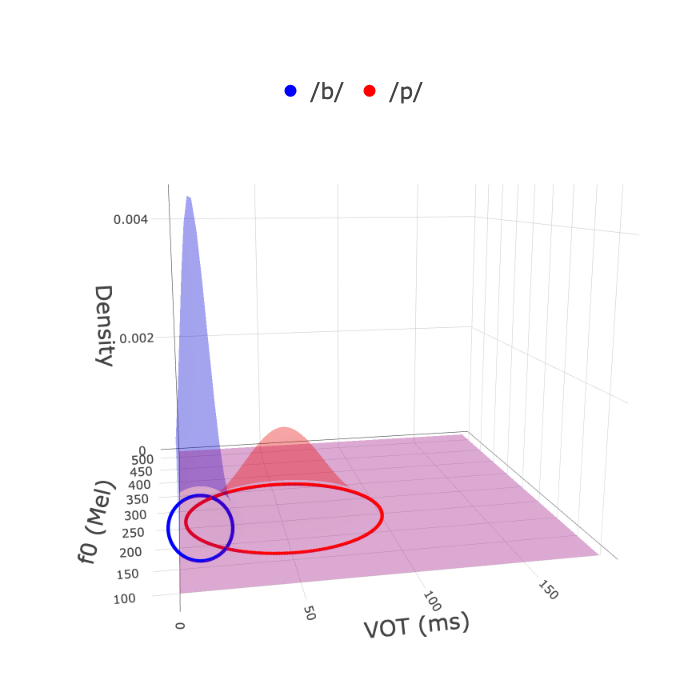
\includegraphics[width=0.33\linewidth,height=0.49\textheight]{../figures/plotly//p.3d.density.panel_1} }\subfloat[Distributions for /d/ and /t/\label{fig:show-representations-plots-2}]{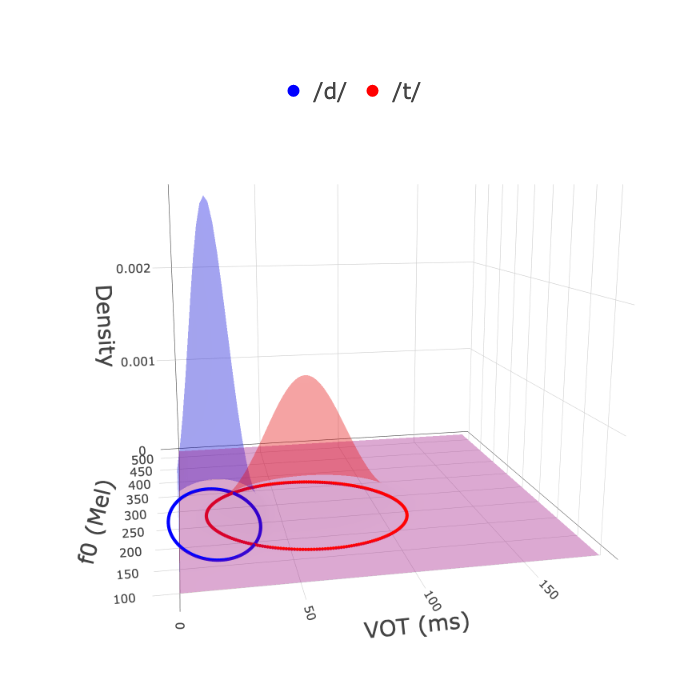
\includegraphics[width=0.33\linewidth,height=0.49\textheight]{../figures/plotly//p.3d.density.panel_2} }\subfloat[Distributions for /g/ and /k/\label{fig:show-representations-plots-3}]{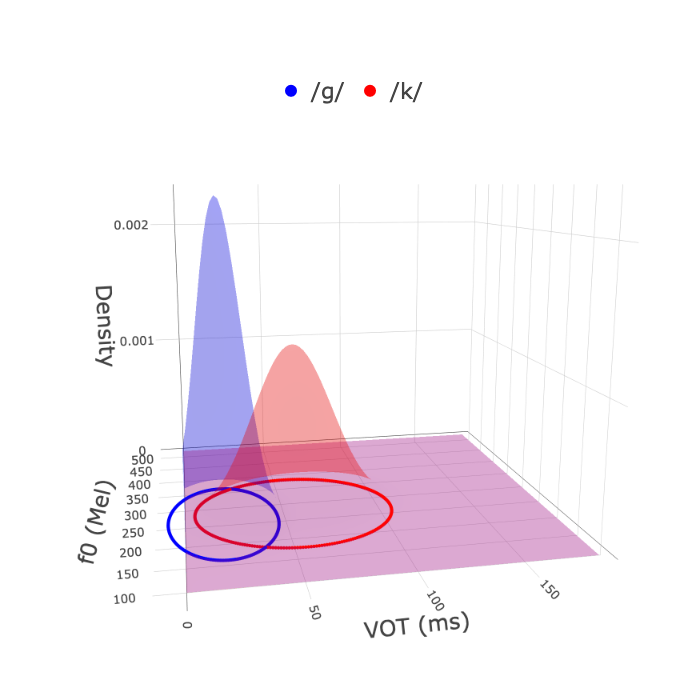
\includegraphics[width=0.33\linewidth,height=0.49\textheight]{../figures/plotly//p.3d.density.panel_3} }\newline\subfloat[Categorization for /b/-/p/\label{fig:show-representations-plots-4}]{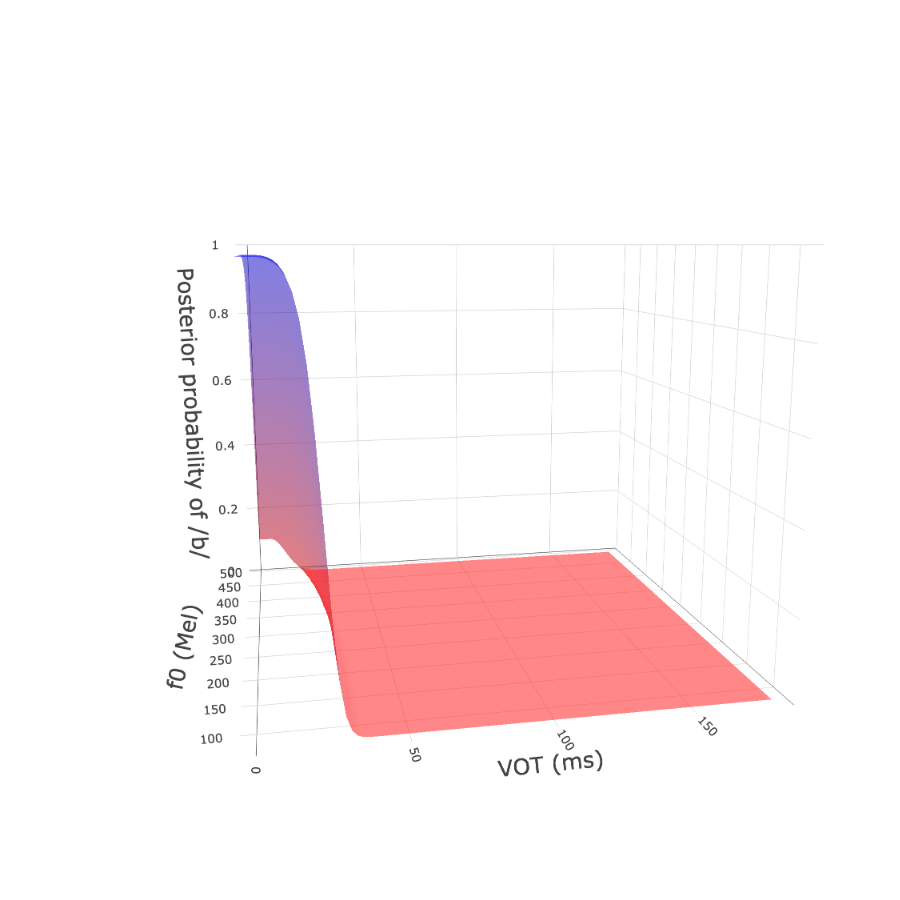
\includegraphics[width=0.33\linewidth,height=0.49\textheight]{../figures/plotly//p.3d.categorization.panel_1} }\subfloat[Categorization for /d/-/t/\label{fig:show-representations-plots-5}]{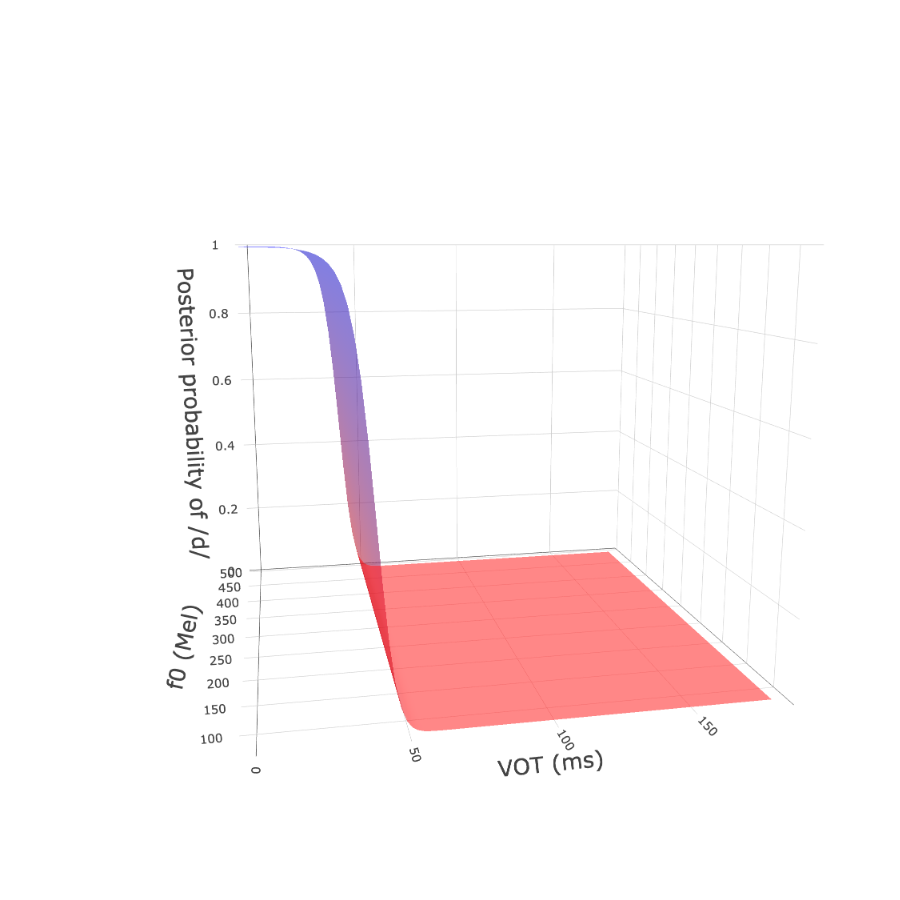
\includegraphics[width=0.33\linewidth,height=0.49\textheight]{../figures/plotly//p.3d.categorization.panel_2} }\subfloat[Categorization for /g/-/k/\label{fig:show-representations-plots-6}]{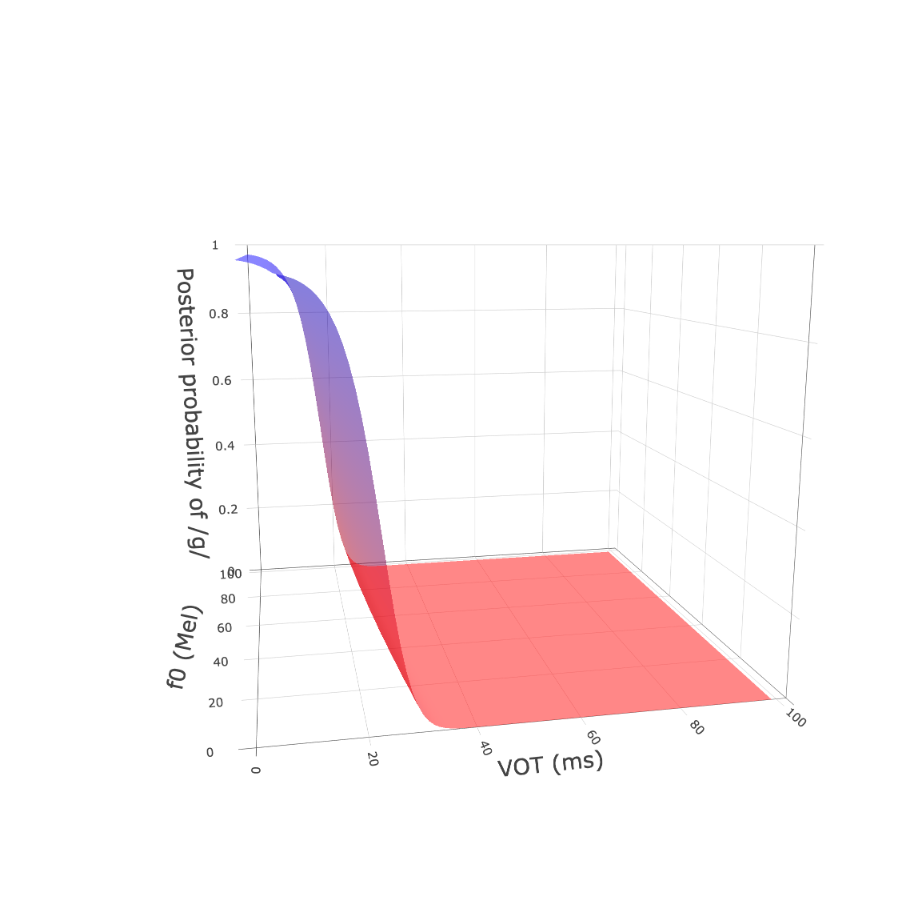
\includegraphics[width=0.33\linewidth,height=0.49\textheight]{../figures/plotly//p.3d.categorization.panel_3} }

}

\caption{Illustrating listeners' implicit category representations. \textbf{Top row:} Bivariate Gaussian category likelihoods learned from (fit to) the by-talker normalized cue distributions in Figure \ref{fig:demonstrate-normalization}B. Ellipses show 95\% probability mass. \textbf{Bottom row:} Categorization functions that would result from these category likelihoods prior to taking into account other effects on decision making (see Figure \ref{fig:show-lapse-bias-demonstration-plots} in the next section).}\label{fig:show-representations-plots}
\end{figure}

\hypertarget{post-linguistic-decision-making-incorporating-priors-response-biases-and-attentional-lapses}{%
\subsection{`Post-linguistic' decision-making: incorporating priors, response biases, and attentional lapses}\label{post-linguistic-decision-making-incorporating-priors-response-biases-and-attentional-lapses}}

The third and final step in our simplified model takes the output of the second step and derives a decision/recognition.\footnote{In some contexts, it can be productive to further split this step into \emph{recognition} of the category and post-recognition processes that affect the behavioral \emph{response}. For the present purpose, we group these processes together. Similarly, some models of perceptual decision-making distinguish between \emph{decision thresholds} (the amount of evidence necessary before a decision is being made) and \emph{decision biases} (stimulus-independent effects on the activation or probability of a response option, \protect\hyperlink{ref-clarkedavidson2008}{Clarke-Davidson et al., 2008}; \protect\hyperlink{ref-venezia2012}{Venezia, Saberi, Chubb, \& Hickock, 2012}). For the present purpose, these two have essentially identical effects.} This includes the integration of information about the prior probability of a category in the current context, \(p(c | context)\). In Bayesian ideal observer models, this integration takes place according to Bayes theorem, yielding an estimate of each category's posterior probability (e.g., \protect\hyperlink{ref-luce-pisoni1998}{P. A. Luce \& Pisoni, 1998}; \protect\hyperlink{ref-norris-mcqueen2008}{Norris \& McQueen, 2008}). Alternative computational approaches can introduce additional degrees of freedom, for example, by allowing non-optimal weighting of priors and category likelihoods. As our goal here is to arrive at as simple a model as possible, we follow the approach taken in ideal observers:

\begin{equation}\label{eq:posterior-probability}
\begin{split}
p(category | input) & = \frac{p(input | c) p(c)}{\Sigma_i p(input | c_i) p(c_i)} \\
                    & = \frac{\mathcal{N}\!(input | \mu_c, \Sigma_c) p(c)}{\Sigma_i \mathcal{N}\!(input | \mu_{c_i}, \Sigma_{c_i}) p(c_i)}
\end{split}
\end{equation}

where the second row substitutes the Gaussian category likelihoods assumed in the previous section into the equation. In Bayesian models, \(p(c_i)\) is generally assumed to reflect a rational estimate based on either the relative frequency of the category in this type of context in listeners' longterm experience or an estimate based on the expectations about the present context. The latter allows for the integration of \emph{response biases} that go beyond capturing the relative frequency of categories in previous experience. In an experiment with a 2AFC task, for example, participants might expect both response options to occur about equally often. This might lead participants to adjust response biases based on the sequence of most recently observed categories. The simplified model in Figure \ref{fig:model-perceptual-decision-making} captures these response biases---regardless of whether they reflect priors based on the relative frequency of categories, meta-reasoning about the structure of experiments, or other factors---through the parameter \(\pi\).
For a \(J\)-way categorical outcome, this introduces \(J-1\) degrees of freedom (since \(\Sigma_i \pi_{c_i} = 1\)) that cannot be independently estimated from phonetically annotated databases. These parameters can, however, often be set based on assumptions about the current task as well as on the extent to which prior expectations about natural language transfer to this task. For example, standard experimental designs provide participants with ample evidence that prior expectations based on the relative frequency of lexical items in natural language use do \emph{not} transfer to the experiment (cf. \protect\hyperlink{ref-jaeger2010}{Jaeger, 2010}). In such contexts, participants might quickly come to adjust their expectations and employ uniform response biases.

In addition to response biases, the model in Figure \ref{fig:model-perceptual-decision-making} includes the possibility that listeners sometimes respond \emph{in}dependent of the stimulus. Stimulus-independent responses can occur, for example, because of attentional lapses. On such occasions, the response is only influenced by the response biases. Lapsing models \emph{without} consideration of responses biases have previously been used in some analyses of exposure effect on speech perception (\protect\hyperlink{ref-clayards2008}{Clayards et al., 2008}; \protect\hyperlink{ref-kleinschmidt-jaeger2016cogsci}{Kleinschmidt \& Jaeger, 2016b}; \protect\hyperlink{ref-mcmurray-jongman2011}{McMurray \& Jongman, 2011}). In our model, we further assume that these response biases on lapsing trials are identical to the responses biases on non-lapsing trials. Also, assuming equal priors for all alternative categories, this yields the following simplified model of the joint effect of attentional lapses and responses biases, where \(\lambda\) is lapse rate---the probability of lapsing:\footnote{Readers familiar with psychometric models might recognize the close relation between Equation \eqref{eq:posterior-probability-lapse} and the standard psychometric model in Wichmann and Hill (\protect\hyperlink{ref-wichmann-hill2001}{2001}): \(\gamma + (1-\gamma-\lambda) F(stimulus | \alpha, \beta)\). In the Wichmann and Hill model, \(\gamma\) describes the floor and \(1-\lambda\) describes the ceiling probability. In Equation \eqref{eq:posterior-probability-lapse}, \(\lambda\) is the lapse rate and \(\pi\) determines how the lapses (and non-lapses) are affected by response biases, resulting in a floor of \(\lambda \pi\) and a ceiling of \(1 - \lambda(1 - \pi)\). For the special case of two Gaussian categories with identical variance along a unidimensional cue continuum, Equation \eqref{eq:posterior-probability-lapse} can be described by Wichmann and Hill's psychometric model if the perceptual model \(F\) is set to be a logistic with appropriate choice of its threshold \(\alpha\) and slope \(\beta\) (cf. \protect\hyperlink{ref-kleinschmidt-jaeger2015}{Kleinschmidt \& Jaeger, 2015, p. 200}).}

\begin{equation}\label{eq:posterior-probability-lapse}
p(category | input) = (1 - \lambda) \frac{\mathcal{N}\!\left( input | \mu_c, \Sigma_c \right) \pi}{\Sigma_i \mathcal{N}\!\left( input | \mu_{c_i}, \Sigma_{c_i} \right) \pi_i} + \lambda \frac{\pi}{\Sigma_i \pi_i}
\end{equation}

In Figure \ref{fig:model-perceptual-decision-making}, the fact that response bias affect listeners' responses in both lapsing and non-lapsing trials is indicated by the two arrows leaving from \(\pi\). Figure \ref{fig:show-lapse-bias-demonstration-plots} visualizes the effects of the two parameters \(\lambda\) and \(\pi\).



\begin{figure}

{\centering \subfloat[$\lambda$ = 0, $\pi_{/d/}=.5$\label{fig:show-lapse-bias-demonstration-plots-1}]{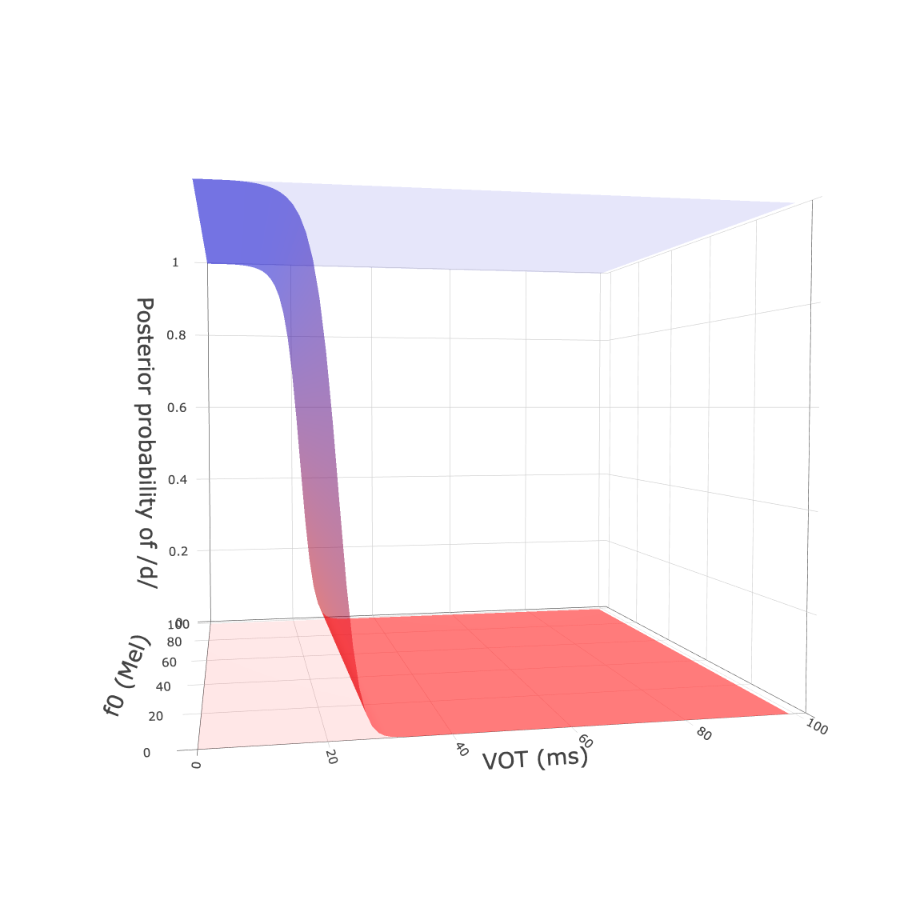
\includegraphics[width=0.49\linewidth,height=0.49\textheight]{../figures/plotly//p.3d.categorization.panel_lambda=1} }\subfloat[$\lambda$ = .2,  $\pi_{/d/}=.5$\label{fig:show-lapse-bias-demonstration-plots-2}]{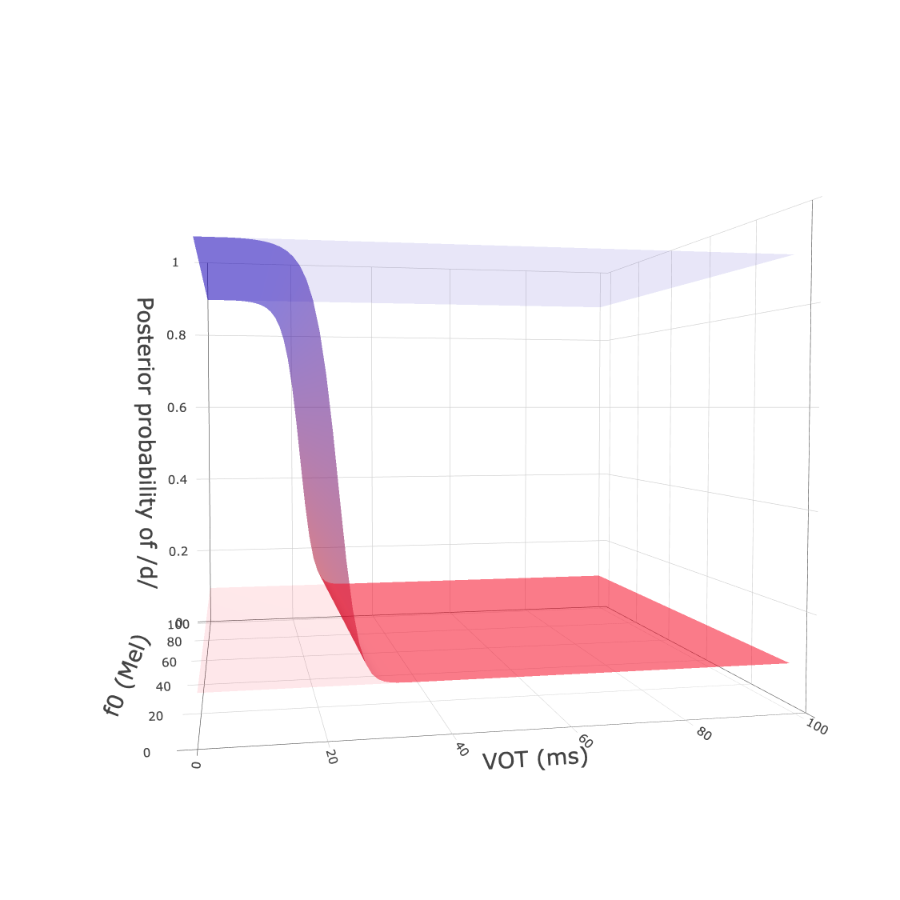
\includegraphics[width=0.49\linewidth,height=0.49\textheight]{../figures/plotly//p.3d.categorization.panel_lambda=2} }\newline\subfloat[$\lambda$ = .2, $\pi_{/d/}=.1$\label{fig:show-lapse-bias-demonstration-plots-3}]{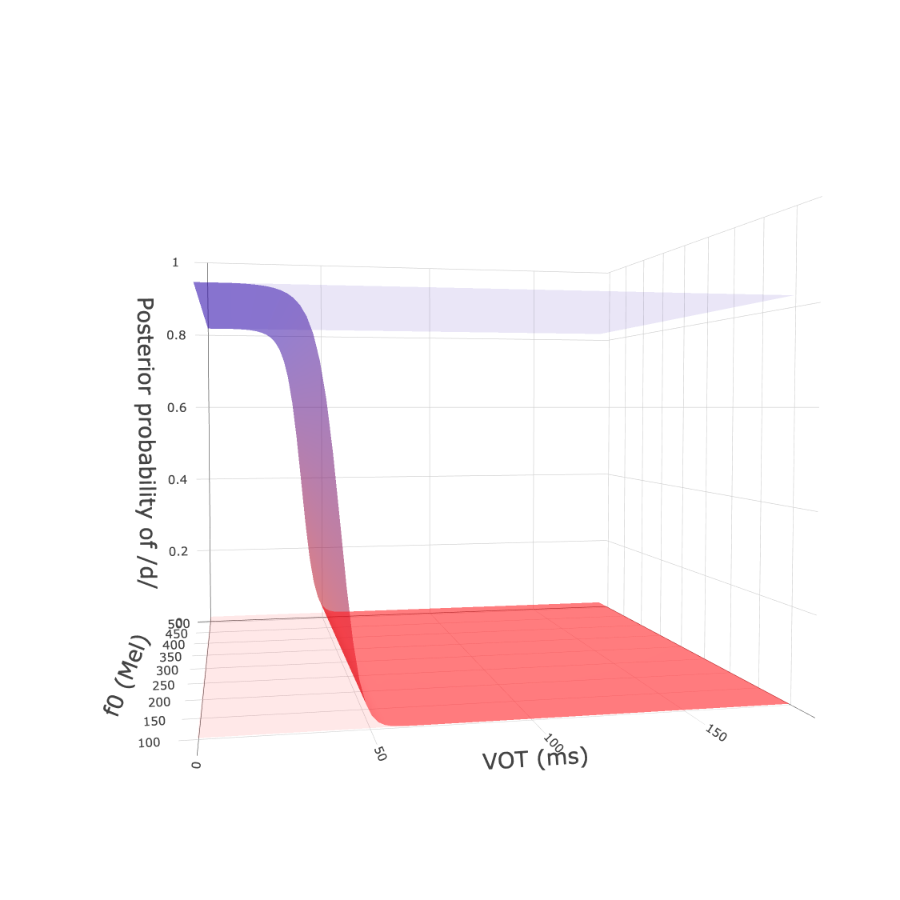
\includegraphics[width=0.49\linewidth,height=0.49\textheight]{../figures/plotly//p.3d.categorization.panel_pi=1} }\subfloat[$\lambda$ = .2, $\pi_{/d/}=.9$\label{fig:show-lapse-bias-demonstration-plots-4}]{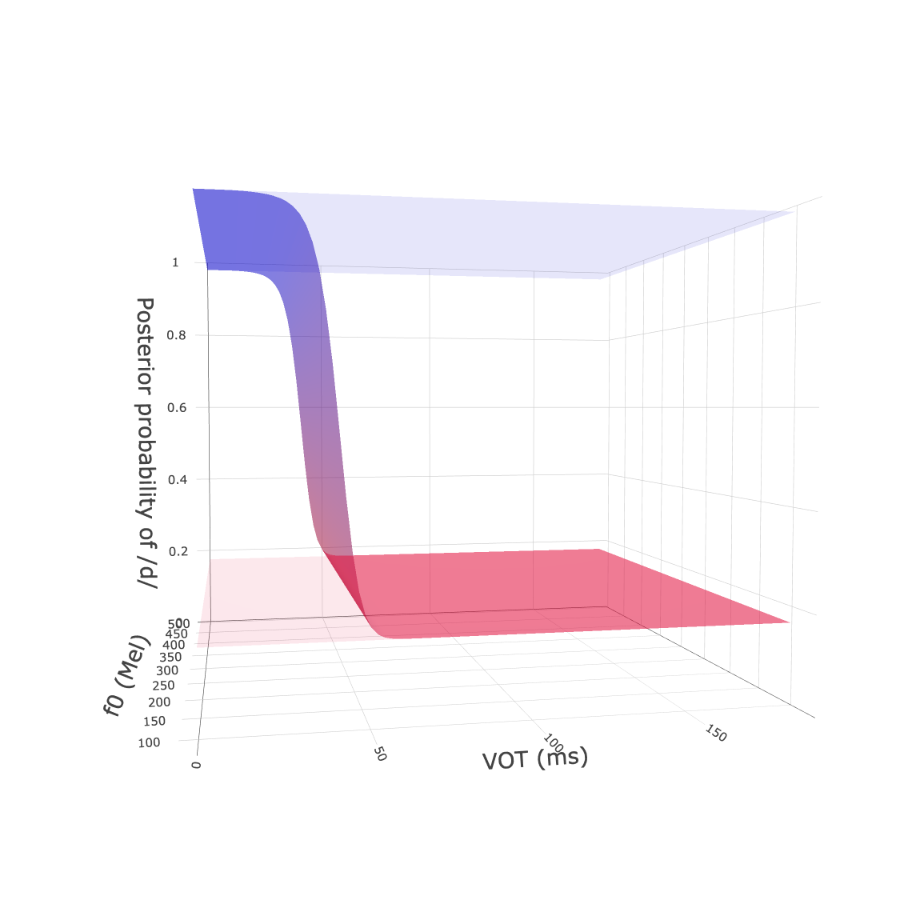
\includegraphics[width=0.49\linewidth,height=0.49\textheight]{../figures/plotly//p.3d.categorization.panel_pi=2} }

}

\caption{Illustrating the effects of \(\lambda\) and \(\pi\) on the posterior probability of /d/, using the two bivariate Gaussian categories of /d/ and /t/ shown in Figure \ref{fig:show-representations-plots}b. The colored planes indicate the ceiling and flooring levels of posterior probability of /d/. Panel a) here is identical to Panel e) in Figure \ref{fig:show-representations-plots},with \(\lambda\) = 0 and \(\pi_{/d/}=.5\). \textbf{Top panel:} Differences in lapse rate \(\lambda\) for a uniform bias of \(\pi_{/d/}=.5\). As the lapse rate increases, the ceiling and flooring responses at the end points change while the categorization slope remains the same. \textbf{Bottom panel:} Differences in bias \(\pi_{/d/}\) when the lapse rate \(\lambda\) = .2. As the bias towards /d/ changes from 0.1 to 0.9, the categorization surface shifts upwards and to the right, resulting in more /d/ responses across the phonetic space.}\label{fig:show-lapse-bias-demonstration-plots}
\end{figure}

The final part of the model is the decision rule that takes the posterior in Equation \eqref{eq:posterior-probability-lapse} as input and returns a response. Here, we follow a common assumption in research in speech perception and employ Luce's choice rule (\protect\hyperlink{ref-luce1959}{R. D. Luce, 1959}; for a comparison of decision rules, see \protect\hyperlink{ref-massaro-friedman1990}{Massaro \& Friedman, 1990}). Under this decision rule, the predicted distribution of responses is identical to the posterior in Equation \eqref{eq:posterior-probability-lapse}. For example, in a 2AFC categorization task, a posterior probability of .3 for /d/ and .7 for /t/ would result in a /d/-response with .3 probability or a /t/-response with .7 probability.

This completes the description of the categorization model in Figure \ref{fig:model-perceptual-decision-making}. For any parameterization of \(\lambda\), \(\pi\), \(\mu_c\), \(\Sigma_c\), and \(\mu\), this model takes acoustic stimuli as input and returns predictions about the expected response distribution (e.g., 30\% /d/-responses and 70\% /t/-responses). Next, we extend this model to capture \emph{changes} at any of the three mechanistic levels. That is, we specify linking hypotheses that describe how the values of \(\pi\), \(\mu_c\), \(\Sigma_c\), and \(\mu\) can change with exposure. Once these linking hypotheses are specified, the model can be used to derive predictions for the distribution of human responses following exposure---for example, during the test phase of an experiment on perceptual recalibration or accent adaptation (see Figure \ref{fig:overview-change}).

\hypertarget{sec:change-normalization}{%
\subsection{\texorpdfstring{Modeling \emph{changes} in normalization}{Modeling changes in normalization}}\label{sec:change-normalization}}

Like many other models of normalization, previous implementations of C-CuRE assumed that the theoretical quantities employed in normalization---for C-CuRE, the means of all cues---are \emph{known} to the listeners (e.g., \protect\hyperlink{ref-apfelbaum-mcmurray2015}{Apfelbaum \& McMurray, 2015}; \protect\hyperlink{ref-mcmurray-jongman2011}{McMurray \& Jongman, 2011}). However, listeners must somehow \emph{infer} these quantities from the observed inputs (see also Section 3.3 in \protect\hyperlink{ref-weatherholtz-jaeger2016}{Weatherholtz \& Jaeger, 2016}). For example, in the types of experiments we consider below, listeners need to \emph{infer} the unfamiliar talker's cue means from the inputs observed during exposure. At the beginning of exposure, the best estimates of the cue means for the unfamiliar talker are the mean expected based on listeners' longterm experience with various different talkers (\(\mu_0\)). With increasing exposure to the unfamiliar talker, listeners can update their estimates of the talker's cue means based on the input. We thus need to expand C-CuRE with a linking hypothesis that describes how listeners update their estimates of the unknown mean---not unlike representational accounts, but only for the \emph{overall} (marginal) distribution of cues, rather than for each category.

Some proposals for such functions include moving-window algorithms that estimate the mean as the sample mean over a finite number of the most recent observations (\protect\hyperlink{ref-lee2002}{Lee, Lau, Wong, \& Ching, 2002}; \protect\hyperlink{ref-zhang-peng2021}{K. Zhang \& Peng, 2021}). Here, we model listeners' estimate of the talker-specific cue mean \(\mu_n\) after \(n\) observations from that talker as simple linear interpolation between the cue mean observed in previous longterm experience (\(\mu_0\)) and the mean observed in the sample observed from the unfamiliar talker (\(\bar{x}\)). This approach has the advantage that listeners can draw on prior experience when they do not yet have much (or any) data from an unfamiliar talker. They can then update the inferred cue mean as they observe further data from the talker (see discussion of the flexibility-stability trade-off in \protect\hyperlink{ref-kleinschmidt-jaeger2015}{Kleinschmidt \& Jaeger, 2015, pp. 178--182}):

\begin{equation}\label{eq:normalization-change}
\mu_n = \frac{1}{\kappa_0 + N} \left( \kappa_0 \mu_0 + N \bar{x} \right) = \frac{\kappa_0}{\kappa_0 + N} \mu_0 + \frac{N}{\kappa_0 + N}\bar{x} 
\end{equation}

The two parameters describing the input from the unfamiliar talker, \(n\) and \(\bar{x}\), are determined by the exposure data used in the experiment (the estimation of the cue means, \(\bar{x}\) requires that the exposure stimuli are phonetically annotated). \(\mu_0\) can be estimated from sufficiently large phonetically annotated databases of speech, essentially assuming that listeners have learned the overall cue means across talkers from previously experienced speech input. This is what we did to create Figure \ref{fig:demonstrate-normalization}, and it is what we assume in the remainder of this study. This leaves only one degree of freedom that is not independently determined: the relative weight of previous experience compared to the input received from the talker so far (\(\kappa_0\)). This is the parameter we vary in the case studies presented below to illustrate the types of results that can be explained through changes in normalization due to recent exposure.

\hypertarget{sec:ideal-adaptor}{%
\subsection{\texorpdfstring{Modeling \emph{changes} in linguistic representations}{Modeling changes in linguistic representations}}\label{sec:ideal-adaptor}}

Just like listeners need to infer an unfamiliar talker's overall cue mean for normalization, listeners who learn talker-specific representations need to infer the \emph{category} means and covariance matrices of the unfamiliar talker. That is, changes in representations can be described as the process of inferring the talker's category likelihood. A theory of this inference process---the ideal adaptor---is introduced in Kleinschmidt and Jaeger (\protect\hyperlink{ref-kleinschmidt-jaeger2015}{2015}). Bayesian belief-updating models based on this theory have been shown to provide a good qualitative and quantitative fit against human responses in results of experiments on perceptual recalibration (\protect\hyperlink{ref-kleinschmidt-jaeger2011}{Kleinschmidt \& Jaeger, 2011}, \protect\hyperlink{ref-kleinschmidt-jaeger2012}{2012}; for closely related models, see \protect\hyperlink{ref-xie2021cognition}{X. Xie, Buxó-Lugo, et al., 2021}), unsupervised or semi-supervised distributional learning (e.g., \protect\hyperlink{ref-kim2020}{D. Kim, Clayards, \& Kong, 2020}; \protect\hyperlink{ref-kleinschmidt-jaeger2016pbr}{Kleinschmidt \& Jaeger, 2016a}; \protect\hyperlink{ref-theodore-monto2019}{Theodore \& Monto, 2019}; for closely related model, see \protect\hyperlink{ref-bejjanki2011}{Bejjanki, Clayards, Knill, \& Aslin, 2011}; \protect\hyperlink{ref-clayards2008}{Clayards et al., 2008}), and accent adapation (\protect\hyperlink{ref-hitczenko-feldman2016}{Hitczenko \& Feldman, 2016}; for a closely related model, see \protect\hyperlink{ref-tan2021}{Tan et al., 2021}). However, as outlined in the introduction, an explicit comparison with alternative models that change normalization or responses biases has been lacking.

The belief-updating model describes the inference of category means and category variances in ways that are conceptually similar to the type of interpolation we described in Equation \eqref{eq:normalization-change}, by combining knowledge based on previously experienced speech input with the observations made from the unfamiliar talker. The specific instance of the model we use here---belief-updating over a Normal-Inverse-Wishart (\(\mathcal{NW^{-1}}\)) prior (\protect\hyperlink{ref-kleinschmidt-jaeger2015}{Kleinschmidt \& Jaeger, 2015})---describes the uncertainty listeners have about the category means \(\mu_c\) and category covariance matrices \(\Sigma_c\) prior to any observations from an unfamiliar talker as a function of four variables (\protect\hyperlink{ref-murphy2012}{Murphy, 2012, pp. 132--133}):

\begin{equation}\label{eq:niw-updating}
\begin{split}
p\left( \mu_c, \Sigma_c | \mathcal{D} \right) & = \mathcal{NW}^{-1} \left( \mu_c, \Sigma_c | \mathrm{m}_{c,0}, \kappa_{c,0}, \nu_{c,0}, \mathrm{S}_{c,0} \right) \\
& = \mathcal{N}\left( \mu_c | \mathrm{m}_{c,0}, \frac{1}{\kappa_{c,0}} \Sigma_{c} \right) \times \mathcal{W}^{-1}\left( \Sigma_c | \mathrm{S}_{c,0}, \nu_{c,0} \right)
\end{split}
\end{equation}

The Normal part of the \(\mathcal{NW^{-1}}\) model describes the uncertainty about the category mean \(\mu_c\), the Inverse-Wishart part describes the uncertainty about the category covariance \(\Sigma_c\). For the former, \(\mathrm{m}_{c,0}\) is the mean of the normal distribution describing the uncertainty about the category mean \(\mu_c\) and \(\kappa_{c,0}\) indicates the extent to which listeners transfer their prior beliefs about the category mean to the present input. The larger \(\kappa_{c,0}\) is, the more certain listeners are about the category mean even prior to any observation, and the less their inferences about the talker's category mean will be influenced by observations from the talker. Put differently, larger \(\kappa_{c,0}\) predicts slower learning of changes in the category mean. Similarly, \(\mathrm{S}_{c,0}\) is the scale matrix of the Inverse-Wishart---having a conceptually similar function to the mean \(\mathrm{m}_{c,0}\) of the Normal distribution---and \(\nu_{c,0}\) indicates extent to which listeners transfer their prior beliefs about the category covariance to the present input. Just as larger \(\kappa_{c,0}\) predicts slower learning of changes in the category mean, larger \(\nu_{c,0}\) predicts slower learning of changes in the category covariances.

In practice, researchers can estimate the \(\mathrm{m}_{c,0}\)s and the \(\mathrm{S}_{c,0}\)s such that they yield the category means and covariances that would be expected given listeners' previous long-term experience.\footnote{That is, \(\mathrm{m_{0,c}} = \mathbf{E}(\mu_c)\) and \(\mathrm{S_{0,c}} = \mathbf{E}(\Sigma)(\nu_{0,c}-D-1)\), where \(D\) is the dimensionality of input (here 1). For details, see Murphy (2012, p.134-5). Additional matching of higher statistical moments should further improve the model.} This leaves two degrees of freedom to model changes in each category's likelihood, \(\kappa_{c,0}\) and \(\nu_{c,0}\). We further follow previous work to make the simplifying assumption that all categories have the same prior \(\kappa_{c,0}\) and \(\nu_{c,0}\) (\protect\hyperlink{ref-kleinschmidt-jaeger2015}{Kleinschmidt \& Jaeger, 2015}, \protect\hyperlink{ref-kleinschmidt-jaeger2016cogsci}{2016b}), leaving just two degrees of freedom \emph{across} all categories to model changes in representations. These are the two parameters we vary in the case studies presented below to illustrate the types of results that can be explained through changes in representations. Figure \ref{fig:demonstrate-niw-prior-mu-sigma} demonstrates how \(\kappa_{c,0}\) and \(\nu_{c,0}\) affect the uncertainty about the category likelihoods for the simple case of univariate Gaussian categories along a single cue dimension (VOT). The case studies we present below employ bivariate categories along f0 and VOT.



\begin{figure}

{\centering \includegraphics{../figures/knitted/demonstrate-niw-prior-mu-sigma-1} 

}

\caption{Illustrating the effects of \(\kappa_{c,0}\) and \(\nu_{c,0}\) on the uncertainty about the category means \(\mu_c\) and variances \(\Sigma_c\) for univariate /d/ and /t/ categories along VOT. The four priors have identical expected category means (\(\mathbf{E}(\mu_{/d/}), \mathbf{E}(\mu_{/t/})\)) and variances (\(\mathbf{E}(\sigma_{/d/}), \mathbf{E}(\sigma_{/t/})\))---set to match the average of the C-CuRE normalized category means and covariance matrices obtained from the data in Chodroff and Wilson (\protect\hyperlink{ref-chodroff-wilson2018}{2018}), and indicated by black points. The four priors differ, however, in their uncertainty about the category means and variances and thus in the changes they predict to occur when exposed to input from an unfamiliar talker. The more uncertain a listener is about the category means and variances of an unfamiliar talker (smaller \(\kappa_{c,0}\) and \(\nu_{c,0}\)), the quicker that listener will adjust their expectations based on the inputs observed from that talker (see Figures \ref{fig:demonstrate-changes-in-representations} and \ref{fig:demonstrate-changes-in-representations-b}). Density lines are drawn at \(10^{-3}\) to \(10^{-10}\) at powers of 10.}\label{fig:demonstrate-niw-prior-mu-sigma}
\end{figure}

As listeners observe additional information from the unfamiliar talker, they update their beliefs (and thus uncertainty) about the distribution of that talker's category means and covariances. The updating of the four \(\mathcal{NW^{-1}}\) parameters after \(N\) observations of a category \(c\) from the talker is described by the equations in \eqref{eq:niw-updating-parameters}, and is deterministic (for details and derivation, see \protect\hyperlink{ref-murphy2012}{Murphy, 2012, p. 134}). \(\kappa_c\) and \(\nu_c\) simply increase by 1 with each observation, capturing the fact that each observation adds additional information about the talker's category mean and covariances. \(\mathrm{m}_{N,c}\) is a weighted combination of its prior value \(\mathrm{m}_{0,c}\) and the category mean of the \(N\) observations \(\bar{x}\)---following the same logic that we applied to the inference of the overall cue mean in Equation \eqref{eq:normalization-change}. Similarly, \(\mathrm{S}_{N,c}\) is a weighted combination of its prior value \(\mathrm{S}_{0,c}\) and the category variability of the \(N\) observations,\footnote{\(\mathrm{S}_c \triangleq \Sigma_{i=1}^N x_{i,c} x_{i,c}^T\) is the uncentered sum of squares matrix of the \(N\) observations (\protect\hyperlink{ref-murphy2012}{Murphy, 2012}).} plus an additional term that captures the uncertainty about the category mean. The SI (\ref{sec:SI-models-changes-in-representations}) summarizes the information in Equations \eqref{eq:niw-updating}-\eqref{eq:niw-updating-parameters} as a graphical model.

\begin{equation}\label{eq:niw-updating-parameters}
\begin{split}
\mathrm{m}_{N,c} & = \frac{\kappa_{0,c} \mathrm{m}_{0,c} + N \bar{x}}{\kappa_{N,c}} = \frac{\kappa_{0,c}}{\kappa_{0,c} + N} \mathrm{m}_{0,c} + \frac{N}{\kappa_{0,c} + N}\bar{x}_c \\
\kappa_{N,c} & = \kappa_{0,c} + N \\
\nu_{N,c} & = \nu_{0,c} + N \\
\mathrm{S}_{N,c} & = \mathrm{S}_{0,c} + \mathrm{S}_{\bar{x}_c} + \frac{\kappa_{0,c} N}{\kappa_{0,c} + N}\left( \bar{x}_c-\mathrm{m}_{0,c} \right) \left( \bar{x}_c-\mathrm{m}_{0,c} \right)^T \\
 & = \mathrm{S}_{0,c} + \mathrm{S}_c + \kappa_{0,c} \mathrm{m}_{0,c} \mathrm{m}_{0,c}^T - \kappa_{N,c} \mathrm{m}_{N,c} \mathrm{m}_{N,c}^T
\end{split}
\end{equation}

The \(\kappa_{c}\)s and \(\nu_{c}\)s are also sometimes called ``pseudocounts'' because they have a rather intuitive interpretation: the value of these parameters can be seen as describing the number of observations of this category that the listener assumes to have observed from the talker. For example, a listener with \(\kappa_{c,0} = 100\) updates her beliefs about an unfamiliar talker's category mean as if she has already seen 100 observations of that category from the talker \emph{prior to having received any input from that talker}. After 900 observations of that category from the unfamiliar talker, this listener's belief about the talker's category mean would be 10/90 mixture of the prior \(\mathrm{m}_{c,0}\) and the mean of the 900 observed category instances \(\bar{x}_c\).

Figures \ref{fig:demonstrate-changes-in-representations} and \ref{fig:demonstrate-changes-in-representations-b} further illustrate how speech input from a talker with unexpected pronunciations changes listeners' beliefs about the category likelihoods and, consequently, their categorization functions. We exposed the four models from Figure \ref{fig:demonstrate-niw-prior-mu-sigma}---each of which reflects the expected category means and variances derived from Chodroff and Wilson (2018), but with different certainty---to input from a talker with unexpected pronunciations of /d/ and /t/. Specifically, the talker's /d/ and /t/ categories were shifted by +25 msecs VOT compared to a (C-CuRE normalized) talker in Chodroff and Wilson' (2018) data. Additionally, the talker's /t/-category exhibited half the variance found in Chodroff and Wilson' data. Figure \ref{fig:demonstrate-changes-in-representations} shows how the expected category likelihoods of the the four models change as a function of input from the new talker. Models with weak prior beliefs about category means (\(\kappa_{0,c}=4\)) accommodate the unfamiliar speech input by changing beliefs about the category mean---shifting categories `horizontally'. Models with weak prior beliefs about category variance (\(\nu_{0,c}=4\)) accommodate the unfamiliar speech input by changing beliefs about the category variance---expanding the category. This is particularly apparent for the /d/ category. Figure \ref{fig:demonstrate-changes-in-representations-b} demonstrates the consequences of these changes for the expected categorization function.



\begin{figure}

{\centering \animategraphics[,controls,loop]{5}{../figures/knitted/demonstrate-changes-in-representations-}{1}{100}

}

\caption[Illustrating the effects of \(\kappa_{c,0}\) and \(\nu_{c,0}\) on changes in the expected category likelihoods, assuming a binary phonetic contrast between two Gaussian categories (/d/-/t/) along a unidimensional continuum (VOT). Updating is shown for the data points in the rug along the x-axis: 20 observations each of /d/and/t/ from a talker who realized both categories with a shifted mean of 25 msec, and exhibits typical variance for /d/ but only half of the typical variance for /t/. We set the lapse rate \(\lambda = 0\) and response biases to uniform (\(\pi_{0,c}=.5\)). Animation controls require Acrobat PDF reader.]{Illustrating the effects of \(\kappa_{c,0}\) and \(\nu_{c,0}\) on changes in the expected category likelihoods, assuming a binary phonetic contrast between two Gaussian categories (/d/-/t/) along a unidimensional continuum (VOT). Updating is shown for the data points in the rug along the x-axis: 20 observations each of /d/and/t/ from a talker who realized both categories with a shifted mean of 25 msec, and exhibits typical variance for /d/ but only half of the typical variance for /t/. We set the lapse rate \(\lambda = 0\) and response biases to uniform (\(\pi_{0,c}=.5\)). Animation controls require Acrobat PDF reader.}\label{fig:demonstrate-changes-in-representations}
\end{figure}



\begin{figure}

{\centering \animategraphics[,controls,loop]{5}{../figures/knitted/demonstrate-changes-in-representations-b-}{1}{100}

}

\caption[Changes in expected categorization functions resulting from the changes in the expected category likelihoods in Figure \ref{fig:demonstrate-changes-in-representations}. We set the lapse rate \(\lambda = 0\), the prior lapse biases to uniform (\(\pi_{0,c}=.5\)). Neither normalization, nor response biases changed as a function of the input. Animation controls require Acrobat PDF reader.]{Changes in expected categorization functions resulting from the changes in the expected category likelihoods in Figure \ref{fig:demonstrate-changes-in-representations}. We set the lapse rate \(\lambda = 0\), the prior lapse biases to uniform (\(\pi_{0,c}=.5\)). Neither normalization, nor response biases changed as a function of the input. Animation controls require Acrobat PDF reader.}\label{fig:demonstrate-changes-in-representations-b}
\end{figure}

\hypertarget{sec:change-bias}{%
\subsection{\texorpdfstring{Modeling \emph{changes} in decision-making}{Modeling changes in decision-making}}\label{sec:change-bias}}

Finally, we specify a linking hypothesis for changes in response biases. To the best of our knowledge, this problem has not previously been formalized, or at least not for speech perception. Initially, we considered two conceptual models, both of which describe changes in response biases that only depend on the category label rather than the specific speech input. One possibility assumes that listeners aim to infer the relative probability of each category based on recent input, and that response biases reflect these estimates. For example, listeners might enter an experiment with expectations about the relative probability of each category based on their relative frequency in previously experienced input, and then update their expectations based on the relative frequency of the categories within the experiment (cf.~belief-updating models of syntactic adaptation, \protect\hyperlink{ref-fine-jaeger2013}{Fine \& Jaeger, 2013}; \protect\hyperlink{ref-jaeger2019}{Jaeger, Burchill, \& Bushong, 2021}; \protect\hyperlink{ref-prasad2021}{Prasad \& Linzen, 2021}). It is, however, clear that such a model could not possibly explain the exposure-based effects typically observed in, for example, perceptual recalibration experiments. In typical variants of those experiments, the relative frequency of the two categories does not differ between exposure conditions.

A second possibility is more plausible: listeners might adapt their response biases based on the categorization errors they make. Consider a typical experiment on accent adaptation. A listener unfamiliar with the target L2 accent will initially miscategorize inputs. Typically, these errors will not be random, but rather exhibit directionality. For example, in experiments on Mandarin-accented English, L1-English participants initially mishear voiced syllable-final stops as voiceless (e.g., hearing \emph{lid} as \emph{lit}, \protect\hyperlink{ref-flege1992}{Flege, Munro, \& Skelton, 1992}; \protect\hyperlink{ref-xie2016jep}{X. Xie et al., 2016}). Since experiments of this type employ exposure stimuli that effectively label the input category (e.g., \emph{lemona\_e}), these mistakes will often become apparent to the participant. Listeners who repeatedly observe themselves making such errors could thus increase the bias for the category that they keep failing to observe (/d/ in this example).\footnote{We thank Zach Burchill for bringing this possibility to our attention.} The idea described here is captured by error-based learning models, including connectionist (\protect\hyperlink{ref-mcclelland-elman1986}{McClelland \& Elman, 1986}; e.g., \protect\hyperlink{ref-rumelhart-mcclelland1986}{Rumelhart \& Mcclelland, 1986}), Bayesian (\protect\hyperlink{ref-jaeger2019}{Jaeger et al., 2021}; \protect\hyperlink{ref-jaeger-snider2013}{Jaeger \& Snider, 2013}), and predictive coding models (\protect\hyperlink{ref-rao-ballard1999}{Rao \& Ballard, 1999}; e.g., \protect\hyperlink{ref-sohoglu2012}{Sohoglu, Peelle, Carlyon, \& Davis, 2012}; for review, see \protect\hyperlink{ref-clark2013}{Clark, 2013}). Here we use a highly simplified version of such a linking hypothesis. Each time an input labeled as category \(c\) is not heard as category \(c\) (i.e., \(\epsilon\mathrm{:}\ c \rightarrow \neg c\)), the log-odds for category \(c\) are increased by a constant amount \(\beta_{\pi}\). And each time, an input that is labeled as another category is heard as category \(c\) (i.e., \(\epsilon\mathrm{:}\ \neg c \rightarrow c\)), the log-odds for category \(c\) are \emph{de}creased by the same constant amount \(\beta\). Thus, after \(n\) observations with \(n_{\epsilon\mathrm{:}\ c \rightarrow \neg c} + n_{\epsilon\mathrm{:}\ \neg c \rightarrow c}\) errors:

\begin{equation}\label{eq:bias-updating}
\begin{split}
\mathrm{logit}(\pi_{n,c}) & = \mathrm{logit}(\pi_{0,c}) + \beta_{\pi} n_{\epsilon\mathrm{:}\ c \rightarrow \neg c} - \beta_{\pi} n_{\epsilon\mathrm{:}\ \neg c \rightarrow c} \\
                          & = \mathrm{logit}(\pi_{0,c}) + \beta_{\pi} (n_{\epsilon\mathrm{:}\ c \rightarrow \neg c} - n_{\epsilon\mathrm{:}\ \neg c \rightarrow c}) \\
                          & := \mathrm{logit}(\pi_{0,c}) + \beta_{\pi} \delta_{\epsilon} \\
\end{split}
\end{equation}

where \(\delta_\epsilon\) is a shorthand for the difference in the two error counts, and \(\pi_{0,c}\) is the initial bias prior to any exposure. In the case studies presented below, we assume a uniform initial bias across all categories, leaving \(\beta_{\pi}\) as the only degree of freedom. For the simple case of a 2AFC task, changes in the bias after \(n\) observations are described by a logistic regression with intercept \(\mathrm{logit}(\pi_{0,c})\) and slope \(\beta_{\pi}\):

\begin{equation}\label{eq:bias-probability}
\begin{split}
\pi_{n,c} = \mathrm{logit}^{-1}\frac{1}{1+ e^{\mathrm{logit}(\pi_{0,c}) + \beta_{\pi} \delta_{\epsilon}}}
\end{split}
\end{equation}

This is the change model for response biases we assume in the remainder of the paper. Figure \ref{fig:demonstrate-lapse-bias-change} illustrates this change model for three different values of \(\beta_\pi\) when the lapse rate \(\lambda=0\). The input to this model is identical to the one used in the previous section to demonstrate changes in representations. The right panel highlights a notable limitation in the types of results that can be explained through changes in responses biases: in the absence of lapses, changes in response biases can only explain \emph{additive} effects on the log-odds of the categories, but not changes in the \emph{slope} of the categorization function (in log-odds). To see how this limitation arises, how the \emph{log-odds} of a category---e.g., /d/---in in Equation \eqref{eq:posterior-probability-lapse} depend on the responses biases \(\pi\):

\begin{equation}\label{eq:posterior-probability-lapse-PR}
\begin{split}
p(/d/ | input) & = \frac{\mathcal{N}\!\left( input | \mu_{/d/}, \Sigma_{/d/} \right) \pi_{/d/}}{\Sigma_i \mathcal{N}\!\left( input | \mu_{c_i}, \Sigma_{c_i}\right) \pi_i} \Rightarrow \\
\log \frac{p(/d/ | input)}{1 - p(/d/ | input)} & =  \\
\log \frac{p(/d/ | input)}{p(/t/ | input)} & =  \log \frac{\mathcal{N}\!\left( input | \mu_{/d/}, \Sigma_{/d/} \right) \pi_{/d/}}{\mathcal{N}\!\left( input | \mu_{/t/}, \Sigma_{/t/} \right) \pi_{/t/}} \\
 & = \log \frac{\mathcal{N}\!\left( input | \mu_{/d/}, \Sigma_{/d/} \right)}{\mathcal{N}\!\left( input | \mu_{/t/}, \Sigma_{/t/} \right)} + \log\frac{\pi_{/d/}}{\pi_{/t/}}
\end{split}
\end{equation}

In other words, changes in response biases have additive effects on the log-odds of /d/ when \(\lambda = 0\): adding some arbitrary amount to \(\pi_{/d/}\) in Equation \eqref{eq:posterior-probability-lapse-PR} and subtracting same amount from \(\pi_{/t/}\) (since \(\Sigma_i \pi_i = 1\)) will lift/lower the entire categorization function up or down by a constant amount, independent of the stimulus. This property does not depend on the specific change model assumed in Equation \eqref{eq:bias-probability}. Regardless of the specific way in which response biases change as a function of the input, these changes should have additive effects on the posterior log-odds.
Note, however, that this constraint only applies if \(\lambda = 0\). For \(\lambda \neq 0\), changes in response biases can lead to non-additive changes in the posterior log-odds.\footnote{Specifically: \(\log \frac{p(/d/ | input)}{p(/t/ | input)} = \log \frac{(1-\lambda)\mathcal{N}\!\left( input | \mu_{/d/}, \Sigma_{/d/} \right) + \lambda \left(\Sigma_i \mathcal{N}\!\left( input | \mu_{i}, \Sigma_{i} \right)\pi(c_i)\right)}{(1-\lambda)\mathcal{N}\!\left( input | \mu_{/t/}, \Sigma_{/t/} \right) + \lambda \left(\Sigma_i \mathcal{N}\!\left( input | \mu_{i}, \Sigma_{i} \right)\pi(c_i)\right)} + \log\frac{\pi_{/d/}}{\pi_{/t/}}\).} This is illustrated in Figure \ref{fig:demonstrate-lapse-bias-change-nonzero-lapse}. Changes in the slope of the categorization function (even in log-odds) therefore do \emph{not} rule out explanations in terms of changing response biases, unless it is also shown that the lapse rate is 0.



\begin{figure}

{\centering \animategraphics[,controls,loop]{5}{../figures/knitted/demonstrate-lapse-bias-change-}{1}{100}

}

\caption[Illustrating the effects of \(\beta_{\pi}\) on changes in the categorization function (\textbf{Left:} posterior probability, \textbf{Right:} posterior log-odds). The model has the same uncertain prior beliefs about category mean and variances as the model in Figure \ref{fig:demonstrate-niw-prior-mu-sigma}D (\(\kappa_{0,c} = \nu_{0,c}=0\)). Neither normalization nor prior beliefs about the categories changes as a function of exposure. We set the lapse rate \(\lambda = 0\), the prior lapse biases to uniform (\(\pi_{0,c}=.5\)). The input to this change model is identical to what was used in Figures \ref{fig:demonstrate-changes-in-representations} and \ref{fig:demonstrate-changes-in-representations-b}. Orange arrows indicate the distance between the posterior log-odds resulting from the two most extreme \(\beta_{\pi}\)s. This highlights the fact that changes to responses biases have additive effects on the log-odds of /d/ responses when \(\lambda = 0\). Animation controls require Acrobat PDF reader.]{Illustrating the effects of \(\beta_{\pi}\) on changes in the categorization function (\textbf{Left:} posterior probability, \textbf{Right:} posterior log-odds). The model has the same uncertain prior beliefs about category mean and variances as the model in Figure \ref{fig:demonstrate-niw-prior-mu-sigma}D (\(\kappa_{0,c} = \nu_{0,c}=0\)). Neither normalization nor prior beliefs about the categories changes as a function of exposure. We set the lapse rate \(\lambda = 0\), the prior lapse biases to uniform (\(\pi_{0,c}=.5\)). The input to this change model is identical to what was used in Figures \ref{fig:demonstrate-changes-in-representations} and \ref{fig:demonstrate-changes-in-representations-b}. Orange arrows indicate the distance between the posterior log-odds resulting from the two most extreme \(\beta_{\pi}\)s. This highlights the fact that changes to responses biases have additive effects on the log-odds of /d/ responses when \(\lambda = 0\). Animation controls require Acrobat PDF reader.}\label{fig:demonstrate-lapse-bias-change}
\end{figure}



\begin{figure}

{\centering \animategraphics[,controls,loop]{5}{../figures/knitted/demonstrate-lapse-bias-change-nonzero-lapse-}{1}{100}

}

\caption[Same as Figure \ref{fig:demonstrate-lapse-bias-change} but for a lapse rate \(\lambda=\) 0.05. For such non-zero lapse rates, changes to the response bias have \emph{non}-additive effects on the posterior log-odds. This means that, even in log-odds, changes in response biases can have effects that go beyond \emph{shifts} in category boundaries. Animation controls require Acrobat PDF reader.]{Same as Figure \ref{fig:demonstrate-lapse-bias-change} but for a lapse rate \(\lambda=\) 0.05. For such non-zero lapse rates, changes to the response bias have \emph{non}-additive effects on the posterior log-odds. This means that, even in log-odds, changes in response biases can have effects that go beyond \emph{shifts} in category boundaries. Animation controls require Acrobat PDF reader.}\label{fig:demonstrate-lapse-bias-change-nonzero-lapse}
\end{figure}

Next, we present two case studies that illustrate the predictions of the three change models for two types of paradigms that have been particularly influential: perceptual recalibration (Case Study 1) and accent adaptation (Case Study 2).

\hypertarget{case-study-1-perceptual-recalibration}{%
\section{Case Study 1: perceptual recalibration}\label{case-study-1-perceptual-recalibration}}

The first paradigm---variably known as perceptual or phonetic learning, retuning, or recalibration---exposes listeners to artificially manipulated native (L1) pronunciations. In a seminal study, Norris et al. (\protect\hyperlink{ref-norris2003}{2003}) exposed Dutch listeners to 20 words that contained an {[}f{]} (e.g., ``witlo\emph{f}''---chicory) and 20 words that contained an {[}s{]} (e.g., ``naaldbo\emph{s}''---pine forest), mixed with 160 fillers that did not contain either sound. Between participants, either all instances of {[}f{]} \emph{or} all instances of {[}s{]} were phonetically manipulated so as to make them perceptually ambiguous between {[}f{]} and {[}s{]}. The other sound remained unchanged. A third, baseline, condition left both {[}f{]} and {[}s{]} unchanged. During a subsequent test phase, participants heard instances of an acoustic continuum ranging from clear {[}\ipatext{ɛ}f{]} to clear {[}\ipatext{ɛ}s{]}, and responded whether they heard ``ef'' or ``es''. Norris and colleagues found that the two groups of participants exhibited strikingly different categorization responses during test (see Figure \ref{fig:norris-2003}): compared to participants in the baseline condition, participants who were exposed to shifted {[}f{]} and typical {[}s{]} shifted their categorization boundary (the step along the acoustic {[}\ipatext{ɛ}f{]}--{[}\ipatext{ɛ}s{]} continuum t at which ``ef'' and ``es'' responses are equally likely) away from {[}\ipatext{ɛ}f{]} towards {[}\ipatext{ɛ}s{]}, so that the participants now categorized more tokens along the {[}\ipatext{ɛ}f{]}--{[}\ipatext{ɛ}s{]} continuum as ``ef''; participants who had heard typical {[}f{]} and shifted {[}s{]} did the opposite, shifting their categorization boundary away from {[}\ipatext{ɛ}s{]} towards {[}\ipatext{ɛ}f{]}, categorizing more tokens as ``es''. These changes after exposure to just 20 shifted word recordings were substantial: e.g., the exact same {[}\ipatext{ɛ}f{]}--{[}\ipatext{ɛ}s{]} recording was categorized as ``ef'' more than 80\% of the time by participants in the {[}f{]}-shifted condition but less than 40\% of the time by participants in the {[}s{]}-shifted condition. This finding has been highly influential, with a recent review citing over 200 studies using variants of this paradigm (\protect\hyperlink{ref-theodore2021}{Theodore, 2021}). Boundary shifts like those observed by Norris and colleagues have been demonstrated for an increasing number of phonetic contrasts and languages (e.g., \protect\hyperlink{ref-hanulikova-weber2012}{Hanulíková \& Weber, 2012}; \protect\hyperlink{ref-kraljic-samuel2005}{Kraljic \& Samuel, 2005}, \protect\hyperlink{ref-kraljic-samuel2006}{2006}; \protect\hyperlink{ref-reinisch2013}{Reinisch, Weber, \& Mitterer, 2013}; \protect\hyperlink{ref-sumner2011}{Sumner, 2011}; \protect\hyperlink{ref-vroomen2007}{Vroomen et al., 2007}). We now know that boundary shifts can occur even under attentional load or distraction (\protect\hyperlink{ref-baart-vroomen2010}{Baart \& Vroomen, 2010}; \protect\hyperlink{ref-zhang-samuel2014}{X. Zhang \& Samuel, 2014}; but see \protect\hyperlink{ref-samuel2016}{Samuel, 2016}), even when the sounds are embedded in connected speech rather than isolated words (\protect\hyperlink{ref-eisner-mcqueen2006}{Eisner \& McQueen, 2006}) or in globally accented speech (\protect\hyperlink{ref-reinisch-holt2013}{Reinisch \& Holt, 2013}), after even fewer shifted tokens (e.g., as few as four, \protect\hyperlink{ref-liu-jaeger2018}{L. Liu \& Jaeger, 2018}, \protect\hyperlink{ref-liu-jaeger2019}{2019}), and that they can persist over hours and days (\protect\hyperlink{ref-eisner-mcqueen2006}{Eisner \& McQueen, 2006}; \protect\hyperlink{ref-saltzman-myers2021}{Saltzman \& Myers, 2021}; \protect\hyperlink{ref-vroomen-baart2009}{Vroomen \& Baart, 2009}) though they eventually decay (\protect\hyperlink{ref-samuel2021}{Samuel, Zheng, \& Dumay, 2021}). More recent work has begun to identify the brain regions involved in perceptual recalibration, which range from auditory and superior temporal cortices (\protect\hyperlink{ref-bonte2017}{Bonte et al., 2017}; \protect\hyperlink{ref-kilianhutten2011}{Kilian-Hütten, Vroomen, \& Formisano, 2011}; \protect\hyperlink{ref-myers-mesite2014}{Myers \& Mesite, 2014}; \protect\hyperlink{ref-ullas2020}{Ullas, 2020}), to more frontal and parietal areas (\protect\hyperlink{ref-myers-mesite2014}{Myers \& Mesite, 2014}; \protect\hyperlink{ref-ullas2020}{Ullas, 2020}; \protect\hyperlink{ref-luthra2020}{\textbf{luthra2020?}}; for review, see \protect\hyperlink{ref-guediche2014}{Guediche et al., 2014}).

In a typical perceptual recalibration experiment, participants are randomly assigned to one of two exposure groups that subsequently perform the same test. During exposure, participants hear stimuli that contain a critical phonetic contrast (here: syllable-intial /d/ vs.~/t/, as in \emph{croco\emph{d}ile} or \emph{cafe\emph{t}eria}, Kraljic \& Samuel, 2006), mixed with many fillers that do not contain that phonetic contrast. Between participants, critical exposure stimuli are manipulated with the goal to shift the category boundary along the phonetic contrast into different directions. This is achieved by exposing listeners to \emph{typical} pronunciations from one category and pronunciations of the other category that are acoustically \emph{shifted} towards the point of maximal perceptual ambiguity between the two categories. Which of the two categories is shifted is manipulated between the two exposure groups. To ensure that the shifted stimuli are still recognized as instances of the intended category, stimulus presentation during exposure is typically \emph{labeled} by presenting the critical contrast in lexical or visual contexts that indicate the intended category (e.g., hearing the shifted sound /?dt/ embedded in the lexical context of ``croco\_ile'' would label the shifted sound as a /d/). In a subsequent test phase, both groups of participants then categorize the same test stimuli along an artificially generated acoustic continuum between the two categories. The goal of this test phase is to estimate participants' categorization function for the critical phonetic contrast, and so test stimuli are \emph{unlabeled}. This is achieved by presenting the manipulated continuum in the contexts of a lexical minimal pair (e.g., \emph{dip}-\emph{tip}) or a nonce-word pair (e.g., \emph{idi}-\emph{iti}).

For example, an influential study by Kraljic and Samuel (\protect\hyperlink{ref-kraljic-samuel2006}{2006}) exposed participants to either shifted /d/ and typical /t/ or shifted /t/ and typical /d/. Participants saw 20 typical and 20 shifted tokens (mixed with 160 fillers). Following exposure, participants in both conditions categorized non-word tokens (/\ipatext{ɪ}d\ipatext{ɪ}/-/\ipatext{ɪ}t\ipatext{ɪ}/) tokens along a six-step /d/-/t/ continuum. Figure \ref{fig:kraljic-samuel-2007-replotted} shows the results obtained by Kraljic and Samuel (2006). Although relatively small, a significant perceptual recalibration effect was observed: participants in the /d/-shifted exposure condition were more likely to give ``d''-responses, resulting a categorization function that is shifted rightwards relative to participants in the /t/-shifted condition. This shift in the category boundary is the signature of perceptual recalibration experiments.\footnote{Kraljic and Samuel (2007, p.~6) report only the ranges for the closure and post-burst aspiration combined. The estimates shown here are based on the observation that post-burst aspiration accounts for about \(2/3^{rd}\)s of that combined duration in the exposure stimuli. We also averaged over the ranges for the two talkers employed in the study, as graphs showing the results by talker were not available.}



\begin{figure}

{\centering \includegraphics{../figures/knitted/kraljic-samuel-2007-replotted-1} 

}

\caption{Categorization functions observed during the test phase of the perceptual recalibration experiment presented in Kraljic and Samuel (2006; replotted from Kraljic \& Samuel, 2007, Figure 1). No errorbars were provided in the original, and the original data are no longer available (Samuel, p.c.). The acoustic properties for each test stimulus were not reported but the range of VOTs were described and are shown on the x-axis.}\label{fig:kraljic-samuel-2007-replotted}
\end{figure}

Unfortunately, most published experiments on perceptual recalibration do \emph{not} report the acoustic properties of their stimuli. Some studies provide aggregate information (e.g., \protect\hyperlink{ref-kraljic-samuel2006}{Kraljic \& Samuel, 2006}, \protect\hyperlink{ref-kraljic-samuel2007}{2007}) and very few provide detailed information and visualization (e.g., \protect\hyperlink{ref-drouin2016}{Drouin et al., 2016}).
We therefore generate data based on the same procedure that experimenters use to create and select the stimuli for perceptual recalibration experiments. The details of our stimulus generation approach, which closely follows the procedure described in Kraljic and Samuel (\protect\hyperlink{ref-kraljic-samuel2006}{2006}), are described in the SI (\ref{sec:SI-PR}). These details do not affect the general results we present below. There are merely meant to provide a sufficiently concrete example. Readers can convince themselves of this claim by downloading the \href{https://osf.io/DO-NOT-FORGET-TO-ADD-THE-OSF-URL-HERE-XXX}{R markdown document that this article is generated from}, allowing them to change any of the parameter settings we assume below.

\hypertarget{data}{%
\subsection{Data}\label{data}}

\hypertarget{exposure-phase}{%
\subsubsection{Exposure phase}\label{exposure-phase}}

Figure \ref{fig:PR-exposure-test-plot} shows the stimuli for the exposure and test phases of the experiment. During /d/-shifted exposure, listeners hear \texttt{20} lexically-labeled word recordings containing /d/ shifted towards /t/ and \texttt{20} lexically-labeled word recordings containing typical /t/, mixed in with word and non-word fillers for a total of 200 recordings. As is typical for perceptual recalibration experiments, these fillers are assumed not to contain any information about the VOT distributions of /d/ and /t/, and thus do not affect listeners' beliefs about those distributions. During /d/-shifted exposure, participants hear lexically-labeled \texttt{20} word recordings containing /t/ shifted toward /d/ and \texttt{20} lexically-labeled word recordings containing typical /d/. Shifted recordings are selected to be perceptually half-way between /d/ and /t/.

Readers familiar with perceptual recalibration experiments might find Figure \ref{fig:PR-exposure-test-plot}A puzzling at first glance. It is rare to see the phonetic properties of the stimuli in those experiments summarized or even visualized. And the conventional way of visualizing the results of perceptual recalibration experiments wrongly suggests that the targeted phonetic contrast falls along a single acoustic continuum (see, e.g., Figure \ref{fig:kraljic-samuel-2007-replotted}). This is, however, rather unlikely to be the case: it is well-known that phonological contrasts tend to vary along multiple phonetic dimensions (e.g., \protect\hyperlink{ref-flege1992}{Flege et al., 1992}; \protect\hyperlink{ref-idemaru-holt2020}{Idemaru \& Holt, 2020}; for a particular powerful demonstration, see \protect\hyperlink{ref-mcmurray-jongman2011}{McMurray \& Jongman, 2011}). For the phonetic contrast at hand, VOT is known to be the primary cue to syllable-initial stop voicing in American English, but f0 and other cues also affect listeners' categorization responses (e.g., \protect\hyperlink{ref-burchill-jaeger2022}{Burchill \& Jaeger, 2021}; \protect\hyperlink{ref-idemaru-holt2011}{Idemaru \& Holt, 2011}; \protect\hyperlink{ref-schertz2015}{Schertz, Cho, Lotto, \& Warner, 2015}; \protect\hyperlink{ref-toscano-mcmurray2012}{Toscano \& McMurray, 2012}).
Although not strikingly evident in Figure \ref{fig:PR-exposure-test-plot}A, this also applies to the /d/-/t/ contrast: /d/ and /t/ vary along both VOT and f0 among other cues (e.g., \protect\hyperlink{ref-chodroff-wilson2018}{Chodroff \& Wilson, 2018}; \protect\hyperlink{ref-kirby2020}{Kirby, Kleber, Siddins, \& Harrington, 2020}; \protect\hyperlink{ref-schertz2015}{Schertz et al., 2015}).\\



\begin{figure}

{\centering \includegraphics{../figures/knitted/PR-exposure-test-plot-1} 

}

\caption{Distribution of the exposure and test of the perceptual recalibration experiment. \textbf{Panel A - Exposure:} 20 tokens each of shifted and typical /d/ and /t/, respectively. Arrows indicate how the shifted tokens created by the experimenter differ from typical tokens of the same category (arrows originate from the mean of typical tokens and end at the mean of shifted tokens). As would be expected given the procedures researchers typically employ to generate stimuli for this type of experiment, the exposure distributions for /d/ and /t/ in both conditions differ primarily along VOT but, notably, \emph{also} differ along f0. \textbf{Panel B - Test (identical for both exposure groups):} Numbers indicate the item ID of the test tokens used in subsequent plots, with IDs in increasing order corresponding to 85\%, 65\%, 55\%, 45\%, 35\%, 15\% expected /d/-responses \emph{prior to exposure} (e.g., in a test-only norming experiment).}\label{fig:PR-exposure-test-plot}
\end{figure}

\hypertarget{test-phase}{%
\subsubsection{Test phase}\label{test-phase}}

The test phase consists of the six stimuli shown in Figure \ref{fig:PR-exposure-test-plot}B, chosen to yield 15\%, 35\%, 45\%, 55\%, 65\%, 85\% expected /d/-responses in a norming experiment without any prior exposure to the talker's speech. This closely resembles the test stimulus placement typical for perceptual recalibration experiments, which tend to examine tokens at the two ends of the continuum as well as those placed near the category boundary. Note that our simulations predict the effects at the \emph{beginning} of the test phase, prior to repeated exposure to the same stimuli over the course of testing. Recent work found that this repeated testing \emph{reduces} the effects of exposure (\protect\hyperlink{ref-liu-jaeger2018}{L. Liu \& Jaeger, 2018}, \protect\hyperlink{ref-liu-jaeger2019}{2019}; \protect\hyperlink{ref-luthra2020}{\textbf{luthra2020?}}; for review, see \protect\hyperlink{ref-theodore2021}{Theodore, 2021}). As a consequence, averaging across all test blocks---as is commonly done---underestimates the effects of exposure (for early mention of this concern, see \protect\hyperlink{ref-norris2003}{Norris et al., 2003, p. 11}).

\hypertarget{results}{%
\subsection{Results}\label{results}}

Next, we use the models introduced in Section \ref{sec:framework} to illustrate to what extent changes in normalization, representations, or response biases can explain the typical behavioral signature of perceptual recalibration experiments: a shift in the category boundary in the same direction as the shifted tokens during exposure (optionally accompanied by a change in slope of the categorization functions). The goal of these computational demonstrations is to illustrate the general type of pattern that the three different hypotheses can account for.

All three change models start from the same prior state. Specifically, we assume that listeners have acquired category representations with expected category means (\(\mathbf{E}(\mu_{/d/}), \mathbf{E}(\mu_{/t/})\)) and variances (\(\mathbf{E}(\sigma_{/d/}), \mathbf{E}(\sigma_{/t/})\)) that reflect the talker-normalized distribution in Chodroff and Wilson (2018; see Figure \ref{fig:show-representations-plots}). Prior to any exposure, decision-making is assumed to employ uniform response biases (\(\pi_{/d/}=\pi_{/t/}=.5\)) and exhibit zero lapse rates. The findings we present below do not qualitatively depend on these specific assumptions. For example, none of the qualitative patterns would change if listeners had non-uniform response biases or non-zero lapse rates at the start of the experiment.

\hypertarget{changes-in-representations}{%
\subsubsection{Changes in representations}\label{changes-in-representations}}

We begin by modeling exposure-driven changes in the mapping from VOT and f0 to the /d/ and /t/ categories. This is arguably the mechanism that is most commonly assumed to underlie the boundary shift observed in perceptual recalibration experiments. Specifically, we use the \(\mathcal{NW}^{-1}\) ideal adaptor model described in Section \ref{sec:ideal-adaptor} while varying the \(\kappa_{0,c}\) and \(\nu_{0,c}\) parameters. We set the other two parameters of the \(\mathcal{NW}^{-1}\) ideal adaptor (\(\mathrm{m}\) and \(\mathrm{S}\)) so that they match the expected mean and covariance of the data in Chodroff and Wilson (\protect\hyperlink{ref-chodroff-wilson2018}{2018}) (as we did in Section \ref{sec:ideal-adaptor}). Normalization and responses biases did not change based on exposure (\(\kappa_0 = \infty\); \(\beta_{\delta_\pi}=0\)).

Figure \ref{fig:PR-result-changes-in-representations} shows the predicted categorization functions after /d/-shifted and /t/-shifted exposure, depending on the strength of the prior beliefs for the category means and variances. We show the results for \(\kappa_{0,c}\)s and \(\nu_{0,c}\)s ranging from 1024 (very slow learning) to 4 (very fast learning). These values are best understood in the context of the number of critical exposure stimuli (20 for each category). For example, a \(\kappa_{0,c}=20\) would mean that the listeners' beliefs about the distribution about the category mean after exposure is a 50/50 mix of their beliefs prior to exposure and the mean of the exposure stimuli (see Equation \eqref{eq:niw-updating}). For \(\kappa_{0,c}=4\), listeners' beliefs about the category mean are thus primarily determined by the mean of the exposure stimuli, whereas a \(\kappa_{0,c}=1024\) essentially means that exposure does not affect listeners' belief about the category mean at all (and mutatis mutandis, for \(\nu_{0,c}\)). As an additional reference, we note the best-fitting \(\kappa_{0,/b/}=\kappa_{0,/p/}=243\) (95\% CI: 163-495) and \(\nu_{0,/b/}=\nu_{0,/p/}=772\) (95\% CI: 493-1180) obtained by Kleinschmidt and Jaeger (\protect\hyperlink{ref-kleinschmidt-jaeger2016cogsci}{2016b}) based on a series of distributional learning experiments on changes only in VOT within a paradigm similar to Clayards et al. (\protect\hyperlink{ref-clayards2008}{2008}). Subsequent improvements to these analyses changed the best-fitting estimates to \(\kappa_{0,/b/}=\kappa_{0,/p/}=160\) (95\% CI: 75-780) and \(\nu_{0,/b/}=\nu_{0,/p/}=510\) {[}95\% CI: 160-1000; Kleinschmidt (\protect\hyperlink{ref-kleinschmidt2019}{2019}){]}.



\begin{figure}

{\centering \includegraphics{../figures/knitted/PR-result-changes-in-representations-1} 

}

\caption{Predictions of a learning model that derives perceptual recalibration as changes in category representations. Predicted categorization responses are shown for the 6 test tokens after /d/- and/t/-shifted exposure, depending on the strength of the prior beliefs in categories means (\(\kappa_{0,c}\)) and covariances (\(\nu_{0,c}\)). Smaller \(\kappa_{0,c}\) and \(\nu_{0,c}\) indicate \emph{faster} learning, weighting previous long-term experience less during the integration with the observations made during the exposure phase of the experiment (see Equation \eqref{eq:niw-updating}). The highlighted panel corresponds to the best-fitting \(\kappa_{0,c}\) and \(\nu_{0,c}\) observed in previous work within other types of paradigms (\protect\hyperlink{ref-kleinschmidt2020}{Kleinschmidt, 2020}; \protect\hyperlink{ref-kleinschmidt-jaeger2016cogsci}{Kleinschmidt \& Jaeger, 2016b}).}\label{fig:PR-result-changes-in-representations}
\end{figure}

Figure \ref{fig:PR-result-changes-in-representations} demonstrates that distributional learning can account for the typical result of perceptual recalibration experiments. Indeed, the parameterization of the \(\mathcal{NW}^{-1}\) ideal adaptor that best fit human responses in a series of distributional learning experiments on /b/ and /p/ (\protect\hyperlink{ref-kleinschmidt2020}{Kleinschmidt, 2020}; \protect\hyperlink{ref-kleinschmidt-jaeger2016cogsci}{Kleinschmidt \& Jaeger, 2016b}) also provides a good qualitative fit against the /d/-/t/ perceptual recalibration results by Kraljic and Samuel (\protect\hyperlink{ref-kraljic-samuel2007}{2007}, gray panel in Figure \ref{fig:PR-result-changes-in-representations}).

We further see that boundary shifts can be the results of either changes in the beliefs about category means (e.g., right column of Figure \ref{fig:PR-result-changes-in-representations}) or changes in the beliefs about category covariances (e.g., bottom row in Figure \ref{fig:PR-result-changes-in-representations}). This is further illustrated by Figure \ref{fig:PR-result-changes-in-representations-categories}, which shows the expected category likelihoods for a subset of the panels of Figure \ref{fig:PR-result-changes-in-representations}. In fact, for the specific experiment simulated here, the latter leads to comparatively larger boundary shifts. This is the result of the experimenter selecting `typical' stimuli as the starting point for the phonetic manipulations. In our simulation, we emulated this by reducing the variance of the stimuli by a constant factor, simulating a process by which the experimenter discards `atypical' recordings. Leaving these specifics aside, this demonstrates that terms like ``category expansion'' and ``boundary shifts'' are best understood as \emph{descriptions} of results, rather than hypotheses about the underlying \emph{mechanisms}. The ideal adaptor and similar learning mechanisms can explain either type of result (\protect\hyperlink{ref-bent-baeseberk2021}{Bent \& Baese-Berk, 2021}; \protect\hyperlink{ref-hitczenko-feldman2016}{Hitczenko \& Feldman, 2016}; for additional support and discussion, see also \protect\hyperlink{ref-kleinschmidt-jaeger2015}{Kleinschmidt \& Jaeger, 2015, p. 168}; \protect\hyperlink{ref-theodore-monto2019}{Theodore \& Monto, 2019}).



\begin{figure}

{\centering \includegraphics{../figures/knitted/PR-result-changes-in-representations-categories-1} 

}

\caption{Expected category likelihoods (based on expected category mean and covariance matrices), depending on the exposure condition and the strength of the prior beliefs in categories means (\(\kappa_{0,c}\)) and covariances (\(\nu_{0,c}\)). Only a illustrative subset of the \(\kappa_{0,c}\) and \(\nu_{0,c}\) values from Figure Figure \ref{fig:PR-result-changes-in-representations} are shown.}\label{fig:PR-result-changes-in-representations-categories}
\end{figure}

Finally, Figure \ref{fig:PR-result-changes-in-representations} shows that distributional learning does not only predict shifts in the category boundary but can also predict changes in the slope of those boundaries. This is evident, for example, in the top-right panel.\footnote{This is still true if the predicted log-odds, rather than proportions, of /d/ are plotted.} Although such changes in slopes are often not discussed, they are present in many perceptual recalibration experiments (see \protect\hyperlink{ref-drouin2016}{Drouin et al., 2016}; \protect\hyperlink{ref-liu-jaeger2018}{L. Liu \& Jaeger, 2018}, \protect\hyperlink{ref-liu-jaeger2019}{2019}; \protect\hyperlink{ref-myers-mesite2014}{Myers \& Mesite, 2014}).

\hypertarget{changes-in-decision-making}{%
\subsubsection{Changes in decision-making}\label{changes-in-decision-making}}

Next, we model the effects of changes in decision-making. In addition to varying the rate at which response biases change \(\beta_{\delta_\epsilon}\), we also vary the lapse rate parameter \(\lambda\). Normalization and representations did not change based on exposure (\(\kappa_0 = \kappa_{0,c} = \nu_{0,c} = \infty\)). To the best of our knowledge, changes in responses biases are \emph{not} commonly considered as an explanation for the boundary shift.



\begin{figure}

{\centering \includegraphics{../figures/knitted/PR-result-changes-in-decision-making-1} 

}

\caption{Predictions of a model that derives perceptual recalibration as changes in decision-making. Predicted categorization responses are shown for the 6 test locations after /d/- and/t/-shifted exposure, depending on the rate at which response biases change (\(\beta_{\pi}\)) and the rate of attentional lapses (\(\lambda_{posterior}\)). The response biases towards /d/ that results from \(\beta_{\pi}\) are shown in the bottom row for each of the two exposure conditions, and are identical within each column (when all trials are lapses, as in the bottom row, the response distribution is identical to the response biases).}\label{fig:PR-result-changes-in-decision-making}
\end{figure}

Figure \ref{fig:PR-result-changes-in-decision-making} shows the effects of changes in response biases for lapse rates ranging from negligible lapse rates (\(\lambda = .0005\), top row) to a scenario in which listeners always lapse (\(\lambda = 1\)). In the latter---rather implausible---edge case, listeners' responses only reflect response biases and are completely stimulus-independent (bottom row). For reference, lapse rates in an experiment that is sufficiently engaging are typically assumed to fall between 1-10\%, with the latter being on the high end (e.g., Clayards et al., 2008 constrained lapse rates to be \(<5\)\%). Kleinschmidt and Jaeger (2016) report a best-fitting value of 5\%.

The primary insight from Figure \ref{fig:PR-result-changes-in-decision-making} is that changes in response biases can account for the type of boundary shift that is observed in perceptual recalibration experiments. This highlights the fact that the signature result of perceptual recalibration experiments is ambiguous between two explanations that evoke very different cognitive architectures. For the case study, perhaps the closest match to the findings from Kraljic and Samuel (2006) is observed for plausible lapse rates up to 5\% and small changes in response bias (second column, top rows).

Figure \ref{fig:PR-result-changes-in-decision-making} further shows that changes in response biases do not necessarily lead to changes that are symmetric around the uniform response biases we assumed as a starting point prior to the experiment (\(\pi_{/d/}=\pi_{/t/}=.5\)). For example for \(\beta_{\pi} = .8\), the /d/-shifted condition results in a /d/-bias of \(\pi_{/d/}=.93\), whereas /t/-shifted condition results in \(\pi_{/d/}=.17\) (\(\neq 1 - .93\)). This type of asymmetry in the degree of change in the response bias is a consequence of the type of change model we assumed in Equation \eqref{eq:bias-updating}---specifically, the assumption that listeners change their responses biases only when their categorization is in conflict with the category label indicated in the input (e.g., when the listener hears a /t/ but the lexical context is \emph{lemona\_e}). This means that the degree to which listeners change their response biases depends on the degree to which the acoustic properties of the exposure stimuli are in conflict with the lexical contexts they appear in.

Finally, Figure \ref{fig:PR-result-changes-in-decision-making} illustrates the effects of lapse rates. The higher the rate of lapsing trials, the more the overall response pattern is determined by the response biases, rather than by stimulus-dependent aspects. This also means that it can be important to keep lapse rates in mind when analyzing the data. Consider, for example, a scenario in which listeners' lapse rates differ after /d/-shifted and /t/-shifted exposure---e.g., because one exposure condition resulted in a more difficult or less engaging task, or in less plausible stimuli. Compare, say, the blue line for \(\beta_{\pi} = .05\), \(\lambda = .005\) against the red line for \(\beta_{\pi} = .05\), \(\lambda = .5\). Analyses that fail to take into account the difference in lapse rates would wrongly conclude that the category representations have changed since the slopes of the categorization functions resulting from the two exposure conditions seem to differ.

\hypertarget{changes-in-normalization}{%
\subsubsection{Changes in normalization}\label{changes-in-normalization}}

Finally, we compare a model that normalizes test tokens based on the phonetic inputs experienced during exposure to a model that continues to apply normalization based on previous longterm experience. The model that changes normalization based on the exposure tokens essentially subtracts the cue means experienced during exposure---which varies based on the exposure condition---from that of each of the test tokens. We implement this by adjusting the cue values of the test tokens by the difference between the prior mean of cues based on previously experienced input (estimated in Section \ref{sec:framework} based on data from \protect\hyperlink{ref-chodroff-wilson2018}{Chodroff \& Wilson, 2018}) and the mean of cues experienced during exposure. All other parameters have the same setting as in the previous section's, except that no changes in representations or response biases were considered.

To illustrate the consequences of normalization, we vary the only parameter of our change model for normalization, \(\kappa_0\). Figure \ref{fig:PR-test-normalization} illustrates the effect of this centering on the perception of test locations, so that normalization \emph{only} depends on the mean of the exposure data (i.e., when listeners have correctly inferred the mean of the test data). Figure \ref{fig:PR-test-normalization} shows the results of different degrees of normalization. Paralleling the results for changes in representations and response biases, changes in normalization can account for the signature boundary shift of perceptual recalibration experiments.



\begin{figure}

{\centering \animategraphics[,controls,loop]{5}{../figures/knitted/PR-test-normalization-}{1}{100}

}

\caption[Effects of changes in normalization on the perception of test locations, depending on the relative weighting of previous experience (\(\kappa_0\)) during the inference of the cue mean during exposure. Normalization based on exposure results in a shift in the perception of the test stimuli. The magnitude of that shift depends on \(\kappa_0\), with larger shifts (more learning) for smaller \(\kappa_0\) (see Equation \eqref{eq:normalization-change}).]{Effects of changes in normalization on the perception of test locations, depending on the relative weighting of previous experience (\(\kappa_0\)) during the inference of the cue mean during exposure. Normalization based on exposure results in a shift in the perception of the test stimuli. The magnitude of that shift depends on \(\kappa_0\), with larger shifts (more learning) for smaller \(\kappa_0\) (see Equation \eqref{eq:normalization-change}).}\label{fig:PR-test-normalization}
\end{figure}



\begin{figure}

{\centering \includegraphics{../figures/knitted/study-PR-models-normalization-results-1} 

}

\caption{Predictions of a model that derives perceptual recalibration from changes in normalization. Predicted categorization responses are shown for the 6 test locations after /d/- and/t/-shifted exposure, depending on the relative weighting of previous experience (\(\kappa_0\)) during the inference of the cue mean during exposure. Smaller \(\kappa_0\) indicate faster learning.}\label{fig:study-PR-models-normalization-results}
\end{figure}

\hypertarget{discussion}{%
\subsection{Discussion}\label{discussion}}

We applied the three change models developed in Section \ref{sec:framework} to a hypothetical experiment within the perceptual recalibration paradigm. All three models predict the characteristic boundary shift observed in perceptual recalibration experiments. At least at the level of analysis that is typically applied in these experiments, the results of perceptual recalibration experiments therefore do \emph{not} provide decisive evidence for changes in representations (contrary to what is often assumed in previous studies since \protect\hyperlink{ref-norris2003}{Norris et al., 2003}). Rather, boundary shifts can be the result of changes at \emph{any} of the three mechanistic levels we have explored here.

This does not mean that perceptual recalibration experiments are \emph{necessarily} uninformative about the mechanisms underlying the effects of recent exposure. If adequate approaches to data analysis are chosen, these experiment do, in principle, provide information that can be used to distinguish between the three different explanations (cf.~the fact that changes in biases are additive in the log-odds of the categorization response). Additionally, specific linking hypotheses---like the ones we have introduced here---can be compared in terms of their \emph{quantitative} fit against the data, while appropriately taking into account their functional flexibility (e.g., through model comparison measures like the Bayesian leave-one-out information criterion, \protect\hyperlink{ref-vehtari2017}{Vehtari, Gelman, \& Gabry, 2017}). Before we discuss this and other ways towards studies that more decisively distinguish between the three explanations, we present a second case study using another very common paradigm.

\hypertarget{case-study-2-accent-adaptation}{%
\section{Case Study 2: accent adaptation}\label{case-study-2-accent-adaptation}}

A second important paradigm exposes listeners to unfamiliar \emph{naturally} accented speech---e.g., dialectal (\protect\hyperlink{ref-smith2014}{R. Smith, Holmes-Elliott, Pettinato, \& Knight, 2014}), varietal (\protect\hyperlink{ref-shaw2018}{Shaw et al., 2018}), or second language (L2) accents (\protect\hyperlink{ref-bradlow-bent2008}{Bradlow \& Bent, 2008}; \protect\hyperlink{ref-eisner2013}{Eisner et al., 2013}; \protect\hyperlink{ref-sidaras2009}{Sidaras et al., 2009}; \protect\hyperlink{ref-weil2001a}{Weil, 2001})---compared to a control condition in which listeners are exposed to a familiar accent (typically a `standard' variety of listeners' L1). Following exposure, listeners in either group are tested for improved comprehension of the unfamiliar accent. In an influential study, Bradlow and Bent (\protect\hyperlink{ref-bradlow-bent2008}{2008}) had listeners transcribe a total of 160 sentences of either Mandarin-accented English or L1-accented English, distributed over two sessions on two separate days. In a subsequent test phase, both groups transcribed Mandarin-accented sentences. Participants who were first exposed to Mandarin-accented English were significantly more accurate during test (over 90\% accuracy compared to about 80\%). This finding, too, has since been replicated and extended (for review, see \protect\hyperlink{ref-baeseberk2020}{Baese-Berk et al., 2020}). We now know that substantially shorter exposure can lead to similarly large improvements in accuracy (e.g., 80 sentences in a single session, about 2-5 minutes of speech, \protect\hyperlink{ref-xie2021jep}{X. Xie, Liu, et al., 2021}), that these can persist over hours and days (\protect\hyperlink{ref-witteman2015}{Witteman, Bardhan, Weber, \& McQueen, 2015}; \protect\hyperlink{ref-xie2018lcn}{X. Xie, Earle, \& Myers, 2018}), and that accent adaptation can sometimes generalize across talkers of the same or similar accents (e.g., \protect\hyperlink{ref-baeseberk2013}{Baese-Berk et al., 2013}; \protect\hyperlink{ref-tzeng2016}{Tzeng et al., 2016}; \protect\hyperlink{ref-xie2021jep}{X. Xie, Liu, et al., 2021}). Facilitatory effects of exposure have also been demonstrated in paradigms that tap into online language processing of naturally accented speech, including cross-modal forced-choice tasks (\protect\hyperlink{ref-clarke-garrett2004}{Clarke \& Garrett, 2004}; \protect\hyperlink{ref-xie2018jasa}{X. Xie, Weatherholtz, et al., 2018}), phonological priming (\protect\hyperlink{ref-eisner2013}{Eisner et al., 2013}; \protect\hyperlink{ref-xie2017}{X. Xie \& Myers, 2017}), and visual world eye-tracking (\protect\hyperlink{ref-dahan2008}{Dahan, Drucker, \& Scarborough, 2008}; \protect\hyperlink{ref-hanulikova-weber2012}{Hanulíková \& Weber, 2012}; \protect\hyperlink{ref-trude2012talker}{Trude \& Brown-Schmidt, 2012}).

Similar to the perceptual recalibration paradigm, accent adaptation is studied by manipulating exposure between participants and then testing all participants on the same test tokens. Unlike in perceptual recalibration experiments, both the exposure and the test stimuli of experiments on accent adaptation tend to employ naturally accented speech (\protect\hyperlink{ref-baeseberk2013}{Baese-Berk et al., 2013}; e.g., \protect\hyperlink{ref-bradlow-bent2008}{Bradlow \& Bent, 2008}; \protect\hyperlink{ref-mitterer-mcqueen2009}{Mitterer \& McQueen, 2009}; \protect\hyperlink{ref-sidaras2009}{Sidaras et al., 2009}; \protect\hyperlink{ref-smith2014}{R. Smith et al., 2014}). Critically, such naturally accented speech typically differs from listeners' expectations in ways that can be considerably more complex than the types of manipulation studied in perceptual recalibration experiments. It is thus not clear whether the same mechanisms that underlie perceptual recalibration also underlie adaptation to natural accents. This question continues to attract attention (see recent reviews, \protect\hyperlink{ref-baeseberk2018}{Baese-Berk et al., 2018}; \protect\hyperlink{ref-bent-baeseberk2021}{Bent \& Baese-Berk, 2021}; \protect\hyperlink{ref-zheng-samuel2020}{Zheng \& Samuel, 2020}) presumably also because its answer determines whether perceptual recalibration and related paradigms---which afford increased control over stimuli characteristics---can shed light on how listeners overcome the challenge of cross-talker variability in everyday speech.

The specific manner in which L2-accented categories differ from their L1 counterparts depends on the sound systems of both languages, including differences in how the talkers' L1 and L2 weight the same cues or even whether a cue is used at all in the realization of a phonological contrast (\protect\hyperlink{ref-harmon2019}{Harmon, Idemaru, \& Kapatsinski, 2019}; \protect\hyperlink{ref-ingvalson2011}{Ingvalson, McClelland, \& Holt, 2011}; \protect\hyperlink{ref-kim2002}{M.-R. Kim, Beddor, \& Horrocks, 2002}; \protect\hyperlink{ref-liu-holt2015}{R. Liu \& Holt, 2015}; \protect\hyperlink{ref-schertz2013}{Schertz, 2013}; \protect\hyperlink{ref-yamada-tohkura1992}{Yamada \& Tohkura, 1992}). For instance, in Korean-accented English, the primary and secondary cues to the word-initial stop voicing (e.g., /d/ and /t/) are reversed compared to L1-accented English: f0, which is the secondary cue to voicing in L1-accented English, outweighs VOT (e.g., \protect\hyperlink{ref-schertz2015}{Schertz et al., 2015}). These differences often cause L2-accented categories to differ from L1-accented categories in terms of their category means, category variances, and category covariances (the category-specific correlation between cues, e.g., \protect\hyperlink{ref-smith2019}{B. L. Smith, Johnson, \& Hayes-Harb, 2019}; \protect\hyperlink{ref-vaughn2019}{Vaughn, 2019}; \protect\hyperlink{ref-wade2007}{Wade et al., 2007}; \protect\hyperlink{ref-xie-jaeger2020}{X. Xie \& Jaeger, 2020}). And these differences are often asymmetrically affecting the categories participating in a phonological contrast. For example, L1-German speakers of English often have non-native realizations of /\ipatext{θ}/ but have no trouble pronouncing /s/, which unlike /\ipatext{θ}/ has a counterpart in their L1. These asymmetries in the production of L2 speech are reflected in L1 listeners' perception of L2-accented speech. For instance, L1-English listeners usually correctly identify German-accented word-final /t/s (e.g., \emph{seat}), but mishear word-final /d/s as devoiced (for other asymmetries, see \protect\hyperlink{ref-schertz2015}{Schertz et al., 2015}; \protect\hyperlink{ref-xie2017}{X. Xie \& Myers, 2017}; \protect\hyperlink{ref-zheng-samuel2020}{Zheng \& Samuel, 2020}).

A typical experiment on accent adaptation randomly assigns participants to either treatment or control exposure. The treatment condition exposes participants to one or more talkers with an unfamiliar accent (e.g., speech from an L2-accented speaker). The control condition typically exposes participants to a familiar L1 accent.
All participants then perform the same test involving comprehension of the unfamiliar L2 accent. Any differences between L1-accented vs.~L2-accented groups' response patterns are taken to be the consequence of exposure to the unfamiliar L2 accent. As in the case of perceptual recalibration discussed above, changes of listeners' perceptual responses in the accent adaptation paradigm are often attributed to the learning and updating of linguistic representations. However, these behavioral changes may actually reflect changes of response biases or low-level signal normalization mechanisms. The goal of our second case study is to explore this possibility.

Compared to perceptual recalibration paradigms, experiments on accent adaptation exhibit more heterogeneity in their designs and tasks. Here we focus on studies in which treatment exposure employs a single talker with the unfamiliar accent, and the test phase heard by both groups of participants employs different stimuli from the same accented talker (e.g., \protect\hyperlink{ref-eisner2013}{Eisner et al., 2013}; \protect\hyperlink{ref-schertz2015}{Schertz et al., 2015}; \protect\hyperlink{ref-xie2017}{X. Xie \& Myers, 2017}). For example, in an exposure-test experiment, X. Xie et al. (\protect\hyperlink{ref-xie2016jep}{2016}) exposed two groups of L1-English listeners to Mandarin-accented speech. In exposure, participants in the treatment group heard 30 words ending in /d/ (e.g., \emph{overload}) together with 60 fillers and 90 nonwords. The /d/-final words were chosen to label the the final sound as /d/. Participants in the control group heard the same recordings except that the 30 /d/-final words were replaced with words that did not contain /d/ (e.g., \emph{animal}).\footnote{This control condition serves as a more conservative control compared to control conditions with L1-accented speech (e.g., \protect\hyperlink{ref-bradlow-bent2008}{Bradlow \& Bent, 2008}; \protect\hyperlink{ref-eisner2013}{Eisner et al., 2013}). It shares the same fundamental design idea though that control exposure provides participants with no (or substantially less) information about the unfamiliar talker's realization of the relevant phonological contrast.}
After exposure, participants in both conditions categorized recordings of 60 minimal /d/-/t/ pairs (e.g., \emph{seed} vs.~\emph{seat}) spoken by the same Mandarin-accented talker. Participants who heard /d/-final words during exposure were more likely to categorize /d/-final words correctly during test, compared to the control condition. At the same time, a non-significant numerical \emph{de}crease in accuracy was observed for /t/-final words (see also \protect\hyperlink{ref-xie2018lcn}{X. Xie, Earle, et al., 2018}). Similar paradigms have yielded similar results for other contrasts and other L1-L2 pairs Eisner et al. (\protect\hyperlink{ref-eisner2013}{2013}).

For Case Study 2, we construct a hypothetical experiment that closely follows this type of design. Listeners are exposed to an L2-accent constructed to exhibit the hallmarks of L2-accented speech mentioned above. For the sake of continuity, we focus on the same syllable-initial /d/-/t/ contrast used in Case Study 1. Specifically, we model the type of situation that occurs in, for example, Korean-accented English---which relies more on f0 rather than VOT to signal word-initial /d/-/t/ contrasts, compared to L1-accented English (e.g., \protect\hyperlink{ref-schertz2015}{Schertz et al., 2015}). Like in Case Study 1, we analyze the data in Case Study 2 following the conventions of the field. For experiments on accent adaptation, this typically means that the facilitatory effects of treatment exposure are assessed through improvements in categorization accuracy during test.

\hypertarget{data-1}{%
\subsection{Data}\label{data-1}}

\hypertarget{exposure-phase-1}{%
\subsubsection{Exposure phase}\label{exposure-phase-1}}

Figure \ref{fig:study-AA-exposure-test-plot}A shows the stimuli for the exposure and test phases of the experiment. In the L2-accented exposure condition, listeners hear 30 word recordings containing L2-accented initial /d/ and 30 word recordings containing L1-accented initial /t/ (plus fillers that do not affect any of the change models). In the control L1-accented exposure condition, listeners hear the same words but from an L1-accented talker.

For L1-accented exposure, the category likelihoods were set to match those observed in Chodroff and Wilson (\protect\hyperlink{ref-chodroff-wilson2018}{2018}), after C-CuRE normalization (i.e., the distributions shown in Figure \ref{fig:demonstrate-normalization}B). This follows the same approach we took for the typical tokens in Case Study 1. For L2-accented exposure, we aimed to mimic the type of scenario commonly observed for L2 accents. Whereas the L2-accented /t/ was given the exact same distribution as the L1-accented /t/, the L2-accented /d/ differed from the L1-accented /d/ both in terms of its location and in terms of its covariance. As a result, the primary cue for L1 listeners (VOT) becomes the secondary cue in the L2-accented speech while preserving the relative ordering between categories (i.e., shorter VOT and lower f0 signaling a /d/ than a /t/ category).

\hypertarget{test-phase-1}{%
\subsubsection{Test phase}\label{test-phase-1}}

During test, listeners from both exposure conditions heard the same set of L2-accented speech. 60 test tokens are randomly sampled from the distribution of each L2-accented category (Figure \ref{fig:study-AA-exposure-test-plot}B).



\begin{figure}

{\centering \includegraphics{../figures/knitted/study-AA-exposure-test-plot-1} 

}

\caption{\textbf{Panel A - Exposure:} Distribution of the stimuli used during the exposure phase of the accent adaptation experiment (30 tokens each of L1-accented and L2-accented /d/ and /t/, respectively). \textbf{Panel B - Test:} Distribution of the stimuli used during the test phase of the accent adaptation experiment. The test tokens come from L2-accented speech (60 tokens per category) and are identical for the two exposure conditions. Ellipses show the 95\% probability mass for the two categories in L2-accented exposure speech.}\label{fig:study-AA-exposure-test-plot}
\end{figure}

\hypertarget{results-1}{%
\subsection{Results}\label{results-1}}

Paralleling Case Study 1, we ask which of the three change models can account for the signature results of accent adaptation experiments. Specifically, we assess for each change model whether it can explain the two type of results observed in, for example, X. Xie et al. (\protect\hyperlink{ref-xie2016jep}{2016}): (1) L2-accented /d/ test tokens should be \emph{a priori} more difficult for L1-English listeners to recognize than L2-accented /t/ test tokens; and (2) L2-accented exposure should lead to a significant increase of recognition accuracy for /d/ test tokens without (equivalently) decreased accuracy for /t/ test tokens.

Previous work has often interpreted such patterns as evidence for \emph{representational} changes (e.g., \protect\hyperlink{ref-bent-baeseberk2021}{Bent \& Baese-Berk, 2021}; \protect\hyperlink{ref-eisner2013}{Eisner et al., 2013}; \protect\hyperlink{ref-sidaras2009}{Sidaras et al., 2009}; \protect\hyperlink{ref-sumner2009}{Sumner \& Samuel, 2009}; \protect\hyperlink{ref-tzeng2016}{Tzeng et al., 2016}; \protect\hyperlink{ref-xie2016jep}{X. Xie et al., 2016}). This might in part due to the assumption that changes in response biases can only explain trade-offs in accuracy: as the accuracy for one category improves, it has to inevitably decrease for the other category. Under this assumption, results like those observed by Xie and colleagues cannot be explained by changes in decision-making. Below we show that this assumption is wrong.

Similarly, pre-linguistic normalization---which is frequently discussed in the context of accommodating inter-talker variability in L1-accented speech---does not seem to be considered a plausible mechanism for accent adaptation. In our review of the literature, we did not find any proposals that attribute accent adaptation solely to pre-linguistic normalization. This is perhaps due to the complex ways in which L2-accented speech tends to differ from L1-accented speech. This makes it appear unlikely that, for example, simple centering would be sufficient to explain the adaptive improvements listeners exhibit with exposure. As in Case Study 1, we first model changes in representations, and then compare them against decision-making and normalization.

\hypertarget{changes-in-representations-1}{%
\subsubsection{Changes in representations}\label{changes-in-representations-1}}

We follow the exact same approach as in Case Study 1, including identical parameter settings.
Figure \ref{fig:AA-result-changes-in-representations} shows the predicted categorization accuracy after exposure to L1- or L2-accented speech, as a function of the strength of the prior beliefs for the category means and variances. As in Case Study 1, we show the results for \(\kappa_{0,c}\)s and \(\nu_{0,c}\)s ranging from 1024 (very slow learning) to 4 (very fast learning).

For L1-accented exposure, the accuracy is always predicted to be much higher high for /t/ than for /d/, indicating that /d/ is often misheard as /t/. This matches the first of the two signature results that is typically observed in studies of this type. One additional finding for the L1-accented condition is of note. Compared across the rows from top to bottom, accuracy improves for models with weaker prior beliefs about the category variances (small \(\nu_{0,c}\), bottom rows of Figure \ref{fig:AA-result-changes-in-representations}). At first blush, this is surprising given that listeners in the L1-exposure condition receive only input that matches their prior L1 expectations and mismatches the L2 speech they receive during test. Learning those exposure statistics is therefore not expected to help. In fact, this is an example of the type of unexpected insight that fully specified linking hypotheses can yield. For this instance of the experiment, it turns out that the L1-accented /d/-exposure stimuli in Figure \ref{fig:study-AA-exposure-test-plot} happen to---by chance---exhibit somewhat larger sample variance along f0 (\(s^2\) = 2,421) than is expected for a typical L1 talker (\(\sigma^2\) = 1,647 based on the data from \protect\hyperlink{ref-chodroff-wilson2018}{Chodroff \& Wilson, 2018}). The L2-accented /d/-exposure stimuli show a similar pattern, albeit slightly less so (sample variance \(s^2\) = 2,213). A learner with weak prior beliefs about the category variance will thus learn to expect a larger category variance during test. This in turn slightly increases the likelihood that the L2-accented /d/ test will be correctly identified during test. This particular result will thus not always replicate if we re-ran the experiment. It is, however, a result that \emph{can} be predicted by the learning model, purely based on the specific statistics of the exposure stimuli.



\begin{figure}

{\centering \includegraphics{../figures/knitted/AA-result-changes-in-representations-1} 

}

\caption{Predictions of a learning model that derives accent adaptation as changes in category representations. Predicted categorization accuracies are shown for the L2-accented test tokens after L1-accented and L2-accented exposure, as a function of the strength of the prior beliefs in category means (\(\kappa_0\)) and covariances (\(\nu_0\)). The average accuracy across all test tokens for each condition is shown above the bars. Error bars show 95\% bootstrapped confidence intervals. The panel with gray highlighting corresponds to the combination of \(\kappa_{0,c}\) and \(\nu_{0,c}\) resulting in the best overall accuracy.}\label{fig:AA-result-changes-in-representations}
\end{figure}

Turning to the critical comparison of the two exposure conditions, Figure \ref{fig:study-AA-exposure-test-plot} shows the second signature result of accent adaptation: recognition accuracy is predicted to increase for /d/ without much (or any) decrease in the recognition accuracy of /t/. The best-performing model predicts a striking increase from 0.67 to 0.93 after L2-accented exposure, compared to L1-accented exposure (+1.9 log-odds).

Looking across the distinct \(\kappa_{0,c}\)s and \(\nu_{0,c}\) values, we make two observations. On the one hand, faster learning of category means is generally beneficial under the current scenario. When listeners' beliefs about category covariances are held constant (i.e., looking within each row), smaller \(\kappa_{0,c}\) values yield higher categorization accuracy. This is a straightforward consequence of the fact that the mean of the /d/ category is shifted in the L2 accents, as shown in Figure \ref{fig:study-AA-exposure-test-plot}. Adapting to the L2 accent thus hinges primarily on learning the new category mean for the /d/ category. On the other hand, updating beliefs about the \emph{variance} too rapidly is not necessarily desirable, as seen by comparing panels within each column. In the current scenario, the \emph{true} underlying variance of /d/ is unchanged between the L1 and the L2 accents. Weaker beliefs about the category covariance thus can run the risk of expanding the categories to a degree that causes miscategorization of relatively ambiguous tokens.

Taken together, these results show that changes in representation---modeled here through the ideal adaptor model---can generally explain the type of result that is taken to be the signature of representational changes---in line with proposals that accent adaptation is driven by representational changes X. Xie, Earle, \& Myers (\protect\hyperlink{ref-xie2016}{2016}).

\hypertarget{changes-in-decision-making-1}{%
\subsubsection{Changes in decision-making}\label{changes-in-decision-making-1}}

As in Case Study 1, we again vary two parameters: the rate at which response biases can change \(\beta_{\delta_\epsilon}\) and the lapse rate \(\lambda\). All other parameters were set in exactly the same way as in Case Study 1. Figure \ref{fig:AA-result-changes-in-decision-making} shows the effects of changes in decision-making across different values of these two parameters.

Paralleling Figure \ref{fig:PR-result-changes-in-decision-making} for perceptual recalibration, the bottom row shows the edge case where \(\lambda=1\), meaning that listeners are always lapsing and thus never responding based on the stimulus. Although highly implausible, this extreme case provides a useful, hypothetical, reference against which the rest of the results can be interpreted. When listeners' categorization is entirely dependent on their response biases, and when the biases do not change from the initial uniform distributions (bottom left panel in Figure \ref{fig:AA-result-changes-in-decision-making}), the accuracy is at chance. \emph{If} the biases change, they change according to perceptual errors that are experienced during exposure (Section \ref{sec:change-bias}). Errors are naturally more frequent in the L2-accented than in the L1-accented exposure conditions, and most commonly involve mishearing /d/ as /t/. As a result, the changes of response-biases are more likely to affect categorization accuracy in the L2-accented exposure condition than in the L1-accented exposure condition. The faster the response biases change (larger \(\beta_{\pi}\)), the greater the differences between the L1- and L2-accented exposure conditions are.



\begin{figure}

{\centering \includegraphics{../figures/knitted/AA-result-changes-in-decision-making-1} 

}

\caption{Predictions of a model that derives accent adaptation as changes in decision-making. Predicted categorization responses are shown for the test tokens after L2-accented and L2-accented exposure, depending on the rate at which response biases change (\(\beta_{\pi}\)) and the rate of attentional lapses (\(\lambda_{posterior}\)).}\label{fig:AA-result-changes-in-decision-making}
\end{figure}

Critically, for plausible lapse rates (\(\lambda < .1\)), changes in response biases result in predictions that closely resemble those for changes in representations. For L1-accented exposure, we again see that /d/ test tokens are categorized substantially less accurately than /t/ test tokens, regardless of the specific value of (\(\beta_{\pi}\)). The second signature result---improved accuracy after L2-accented exposure---is obtained for sufficiently large \(\beta_{\pi}\). Notably, Figure \ref{fig:AA-result-changes-in-decision-making} also shows that changes in response biases can result in \emph{overall} improvements in accuracy, compared to L1-accented exposure (e.g., top right panel). These improvements can achieve levels of improvements that approach those observed for the learning model in the previous section. Thus, changes in response biases do not necessarily result in the type of zero-sum trade-offs that is sometimes attributed to them---accuracy improving for one category at the cost of accuracy for the other category. Indeed, zero-sum trade-offs are only necessarily expected when responses are entirely independent of stimulus properties (bottom row of Figure \ref{fig:AA-result-changes-in-decision-making}).

\hypertarget{changes-in-normalization-1}{%
\subsubsection{Changes in normalization}\label{changes-in-normalization-1}}

Finally, we compare models that normalize test tokens based on the phonetic inputs experienced during exposure to models that continue to apply normalization based on previous long-term L1 experience. We again employ the same parameter settings as in Case Study 1.
Figure \ref{fig:AA-result-changes-in-normalization} shows the predicted categorization accuracy following changes in normalization in L1- and L2-accented exposure conditions. We again obtain both signature results of experiments on accent adaptation. For L1-accented exposure, we continue to see that /d/ test tokens are categorized substantially less accurately than /t/ test tokens. This result does not depend much on the value of \(\kappa_0\), although slightly better performance is observed for small values of \(\kappa_0\).

Critically, changes in normalization can also explain improved recognition accuracy for /d/, as well as overall improvements in recognition accuracy. The highest accuracy is obtained for the fastest changes (smallest \(\kappa_0\)), and it matches that observed for changes in decision-making.



\begin{figure}

{\centering \includegraphics{../figures/knitted/AA-result-changes-in-normalization-1} 

}

\caption{Predictions of a model that derives accent adaptation from changes in normalization, depending on the relative weighting of previous experience (\(\kappa_0\)) during the inference of the cue mean during exposure.}\label{fig:AA-result-changes-in-normalization}
\end{figure}

\hypertarget{discussion-1}{%
\subsection{Discussion}\label{discussion-1}}

Paralleling Case Study 1 on perceptual recalibration, we find that any of the three mechanisms of change can in theory explain the signature results of experiments on accent adaptation. In particular, non-representational mechanisms---normalization and decision-making---can result in complex patterns of changes in categorization accuracies. Contrary to the common assumption, these mechanisms can lead to an \emph{overall} (i.e., across category) improvements in recognition accuracies. Overall improvements in accuracy are thus \emph{not} diagnostic of representational changes.\footnote{Likewise, an absence of overall improvements should not be taken as evidence to reject representational changes, either (cf., \protect\hyperlink{ref-zheng-samuel2020}{Zheng \& Samuel, 2020}). This conclusion is only valid \emph{if successful learning of the exposure statistics} does predict improvements during test. But whether this is the case depends on the exposure and test stimuli---a fact that is sometimes forgotten when interpreting experiments.} This supports the conclusion of Case Study 1: at the level of analysis that is commonly applied in previous work (and thus here), the standard paradigms employed in research on accent adaptation do not directly inform what mechanisms cause the facilitatory effects of exposure. Next, we discuss the consequences of these findings in the broader context of other research. This includes research on accent adaptation and related topics that has pioneered analyses beyond changes in accuracy or processing speed, towards a more in-depth understanding of the link between the acoustic input and perception (e.g., \protect\hyperlink{ref-clare2019}{Clare, 2019}; \protect\hyperlink{ref-idemaru-holt2020}{Idemaru \& Holt, 2020}; \protect\hyperlink{ref-kartushina2015}{Kartushina, Hervais-Adelman, Frauenfelder, \& Golestani, 2015}; \protect\hyperlink{ref-kim2020}{D. Kim et al., 2020}; \protect\hyperlink{ref-schertz2015}{Schertz et al., 2015}; \protect\hyperlink{ref-wade2007}{Wade et al., 2007}).

\hypertarget{general-discussion}{%
\section{General discussion}\label{general-discussion}}

Listeners' ability to adaptively change their interpretation of the speech signal as a function of recent exposure is now understood to play a central role in spoken language comprehension. This insight is in large parts the result of research over the last two decades. In the present study we have focused on two of those lines of research that have been influential in shaping researchers' understanding of adaptive changes in speech perception: perceptual recalibration and accent adaptation. Our computational review of these two approaches suggests that the signature results of these two paradigms do not distinguish between three explanations that have quantitatively different implications for theories of speech perception, linguistic representations, and the relation between social and linguistic cognition. We find that low-level, pre-linguistic signal transformation/normalization or changes in response biases during decision-making are sufficient to explain signature results that are often tied to changes of representations. In what follows, we discuss insights emerging from the current finding, and then we close with recommendations for future experiments on speech perception.

\hypertarget{what-follows-from-our-results-and-what-does-not}{%
\subsection{What follows from our results (and what does not)?}\label{what-follows-from-our-results-and-what-does-not}}

Our case studies suggest that one cannot draw strong conclusions about a presence or absence of representational changes from experiments on perceptual recalibration or accent adaptation. This indeterminacy has potentially far-reaching implications: the assumption that recent exposure can shape linguistic representations, or at least their weighting or selection (\protect\hyperlink{ref-xie2018jasa}{X. Xie, Weatherholtz, et al., 2018}), is central to theories of speech perception (for review, see \protect\hyperlink{ref-hay2019}{Hay et al., 2019}; \protect\hyperlink{ref-kleinschmidt-jaeger2015}{Kleinschmidt \& Jaeger, 2015}; \protect\hyperlink{ref-sjerps2019}{Sjerps et al., 2019}). Evidence supporting this possibility has influenced linguistic theories as well as theories about the interface between social and linguistic cognition (for review, see \protect\hyperlink{ref-foulkes-hay2015}{Foulkes \& Hay, 2015}; \protect\hyperlink{ref-sumner2014}{Sumner et al., 2014}). This does not, of course, mean that normalization, representation, and decision-making mechanisms always predict similar response patterns---they do not. Nor does it mean that the three mechanisms cannot be distinguished from each other experimentally. Before we turn to ways in which this can be achieved, we first discuss other results that speak to the mechanisms underlying changes in speech perception.

One important finding is that the inferred physiology (\protect\hyperlink{ref-krauss2002}{Krauss, Freyberg, \& Morsella, 2002}) or social identity of a talker can affect how her speech is processed and interpreted (e.g., regional origin, \protect\hyperlink{ref-hay-drager2010}{Hay \& Drager, 2010}; \protect\hyperlink{ref-niedzielski1999}{Niedzielski, 1999}; sex, \protect\hyperlink{ref-johnson1999}{Johnson, Strand, \& D'Imperio, 1999}; \protect\hyperlink{ref-strand1999}{Strand, 1999}; age, \protect\hyperlink{ref-walker-hay2011}{Walker \& Hay, 2011}; \protect\hyperlink{ref-skoogwaller2015}{Waller, Eriksson, \& Sörqvist, 2015}; and individual identity, \protect\hyperlink{ref-nygaard1994}{Nygaard et al., 1994}; \protect\hyperlink{ref-remez2018}{Remez et al., 2018}). These and other effects of the situational context (e.g., being in a car, \protect\hyperlink{ref-hay2017}{Hay, Podlubny, Drager, \& McAuliffe, 2017}) suggest that listeners have implicit representations that encode expectations about talkers and types of talkers. These findings do, however, leave open whether these expectations relate to pre-linguistic normalization or to linguistic categories (see also discussion of ``relativization'' in \protect\hyperlink{ref-apfelbaum-mcmurray2015}{Apfelbaum \& McMurray, 2015, pp. 936--938}). They also leave open to what extent recent experience affects speech perception through the same mechanisms that underlie the effects of inferred physiology or social identity. This includes the question of whether and how recent experiences can lead to the learning of new linguistic representations.

Other findings might more directly speak to these questions. We briefly discuss findings we consider particularly informative. To anticipate, however, none of these findings decisively argues for one or the other mechanisms. For example, findings that non-speech stimuli can affect the perception of subsequently played speech stimuli (\protect\hyperlink{ref-holt2005}{L. L. Holt, 2005}, \protect\hyperlink{ref-holt2006}{2006}; \protect\hyperlink{ref-huang-holt2011}{Huang \& Holt, 2011}) are compatible with pre-linguistic normalization accounts but seem to be harder to explain through changes in representations. These findings have, however, been challenged (\protect\hyperlink{ref-pitt2016}{Pitt, Szostak, \& Dilley, 2016}), and accounts of them in terms of representational changes or decision-making are possible. Similarly, there are results that seem to be difficult to explain through C-CuRE normalization or changes in responses biases. Perhaps one of the most important studies in this regard is Clayards et al. (\protect\hyperlink{ref-clayards2008}{2008}) and subsequent replications and extensions (\protect\hyperlink{ref-bejjanki2011}{Bejjanki et al., 2011}; \protect\hyperlink{ref-nixon2016}{Nixon et al., 2016}; \protect\hyperlink{ref-theodore-monto2019}{Theodore \& Monto, 2019}). Clayards and colleagues found that categorization responses can be affected by changes of the category variances, without changes in the category means. Specifically, participants that were exposed to /b/ and /p/ categories with larger variance along VOT exhibited more shallow categorization slopes than participants who were exposed to /b/ and /p/ categories with smaller variance (but the same means as the other condition).

This result is predicted by distributional learning accounts of representational changes (as discussed by \protect\hyperlink{ref-clayards2008}{Clayards et al., 2008}; \protect\hyperlink{ref-kleinschmidt-jaeger2015}{Kleinschmidt \& Jaeger, 2015}) but is not as easily explained by C-CuRE normalization. It does not, however, rule out explanations in terms of other normalization. For example, normalization that standardizes cues relative to expectations, in addition to centering them---which we might call \emph{S}-CuRE (for ``standardizing'')---should be able to account for the findings of Clayards et al.~(2008). Such standardization is part of several of the most influential approaches to formant normalization that have been proposed for the perception of vowels (\protect\hyperlink{ref-johnson2020}{Johnson, 2020}; \protect\hyperlink{ref-lobanov1971}{Lobanov, 1971}; \protect\hyperlink{ref-monahan-idsardi2010}{Monahan \& Idsardi, 2010}). The findings of Clayards et al.~(2008) might also be accounted for by changes in response biases provided that the lapse rate is not zero: recall that changes in responses biases can have non-additive effects when the lapse rate is non-zero (Section \ref{sec:change-bias}). And non-zero lapse rates were indeed observed by Clayards et al.~(2008, Figure 3B and footnote 2). Changes in response biases could thus potentially account for changes in the slope of categorization functions---the result observed in Clayards et al.~(2008).

Brain imaging provides another source of evidence to be considered. For example, shifted categorization boundaries in response to the same physical input have been associated with distinct activities in early auditory regions (anterior PT, \protect\hyperlink{ref-kilianhutten2011}{Kilian-Hütten et al., 2011}), regions implicated in phoneme classification (posterior STG/STS, \protect\hyperlink{ref-bonte2017}{Bonte et al., 2017}; \protect\hyperlink{ref-myers-mesite2014}{Myers \& Mesite, 2014}; \protect\hyperlink{ref-ullas2020}{Ullas, 2020}), as well as regions for talker identity processing (right temporal regions, \protect\hyperlink{ref-luthra2020}{\textbf{luthra2020?}}). The left parietal lobe and the insula, which are implicated in perceptual decision-making (e.g., \protect\hyperlink{ref-dacremont2013}{d'Acremont, Schultz, \& Bossaerts, 2013}; \protect\hyperlink{ref-keuken2014}{Keuken et al., 2014}), have also been shown to exhibit distinct activation for different exposure conditions (\protect\hyperlink{ref-bonte2017}{Bonte et al., 2017}; \protect\hyperlink{ref-myers-mesite2014}{Myers \& Mesite, 2014}; \protect\hyperlink{ref-ullas2020}{Ullas, 2020}). These findings leave open which neural networks are responsible for the behavioral changes observed after recent exposure. Given the wide range of regions found to be involved, all three change mechanisms explored here are possible candidates. For instance, the activation of left parietal lobe might reflect its general role in perceptual decision making (e.g., \protect\hyperlink{ref-dacremont2013}{d'Acremont et al., 2013}; \protect\hyperlink{ref-keuken2014}{Keuken et al., 2014}), or it could be due to a more specific role in phonological processing (e.g., processing abstract category information, \protect\hyperlink{ref-guediche2014}{Guediche et al., 2014}).

One limitation of these works is that the conclusion is based primarily on a binary distinction in a brain region's activation pattern (e.g., activity between categorization trials that a /d/ response is made and those in which a /t/ response is made for the same stimulus). More recently, neuroimaging studies have started to approach questions about the underlying neural mechanisms through multivariate analyses. These analyses are crucial for identifying the encoding of perceptual experiences across a distinct array of experimental conditions. Multivariate analyses can also be more sensitive in detecting fine-grained patterns \emph{within} regions responsible for multiple cognitive demands (e.g., \protect\hyperlink{ref-bonte2017}{Bonte et al., 2017}; \protect\hyperlink{ref-luthra2020}{\textbf{luthra2020?}}). The methodological recommendations we make below may help to generate behavioral responses that enable multivariate analyses required for further dissociation among regions functionally responsible for exposure-driven changes. Another promising avenue is to pair temporally-sensitive techniques with imaging methods with good spatial resolution. For instance, studies using a combination of EEG and MEG have identified key regions that regulate perceptual learning of degraded speech by responding to manipulations of either low-level signal clarity or high-level prior knowledge of the speech content (\protect\hyperlink{ref-sohoglu-davis2016}{Sohoglu \& Davis, 2016}; \protect\hyperlink{ref-sohoglu-davis2020}{Sohoglu \& Davis, 2020}).

In short, while there is now a convergence of different approaches---including both behavioral and neuroimaging paradigms---existing findings leave open what neural and cognitive mechanisms underlie adaptive changes in speech perception. In this context, our case studies support two take-home points: i) that less is known about what mechanisms yield the results of our experiments than seems to be often assumed; and ii) that future research on changes in speech perception stands to benefit greatly from more rigorously defined linking hypotheses. With regard to the former point, we note that the indeterminacy of existing results is even more problematic when we take into account that research often seeks to extrapolate beyond the specific paradigm. For example, one common motivation for perceptual recalibration and other paradigms that employ synthesized or otherwise manipulated speech is that they provide experimenters with increased control over the stimuli and yet can shed light on the mechanisms that underlie adaptation to naturally occurring accents. However, this type of argument---which we have made in our own work---requires certainty that the different paradigms study the same mechanisms. And this means that there is value in extending future applications of these paradigms in ways that allow researchers to determine which mechanism drives their results. The recommendations we present in the next section are meant to move us closer to this goal.

With regard to the latter point, we submit that experimenters ought to operate under the null hypothesis that speech perception is strongly affected by expectations about the distributional realization of linguistic categories based on longterm experience. This assumption is now shared by most theories of speech perception. It is also emphasized by recent reviews of the field, which highlight and make accessible the role of distributional properties of the speech input (\protect\hyperlink{ref-bent-baeseberk2021}{Bent \& Baese-Berk, 2021}; \protect\hyperlink{ref-kurumada-roettger2021}{Kurumada \& Roettger, 2021}; \protect\hyperlink{ref-quam-creel2021}{Quam \& Creel, 2021}; \protect\hyperlink{ref-schertz-clare2020}{Schertz \& Clare, 2020}). Critically, informal reasoning about the consequences of this null hypothesis can quickly gain in complexity, making it more likely that \emph{ad-hoc} or \emph{post-hoc} reasoning results in misleading conclusions. Consider the highly influential study ``The Weckud Wetch of the Wast'' (\protect\hyperlink{ref-maye2008}{Maye et al., 2008}). The study exposed listeners to speech in which the vowel categories had undergone systematic (phonological) shifts. After just 20 minutes of exposure, listeners' interpretation of subsequent speech input from the same talker had changed substantially (for replications and extensions, see also \protect\hyperlink{ref-weatherholtz2014}{Weatherholtz, 2014}). Based on additional control conditions, Maye and colleagues concluded that this finding could not be explained by ``general relaxation of the criterion for what constitutes a good exemplar of the accented vowel category'' but rather argued that participants had learned that the talker's categories were systematically shifted. A recent study revisited this result by formalizing the competing accounts (\protect\hyperlink{ref-hitczenko-feldman2016}{Hitczenko \& Feldman, 2016}) in terms of the same ideal adaptor models that we have employed here (\protect\hyperlink{ref-kleinschmidt-jaeger2015}{Kleinschmidt \& Jaeger, 2015}). Hitzcenko and Feldman found that the results of Maye et al.~(2008) were just as well, if not better, predicted by a learning model that expanded the categories, rather than shifting them.

An analytical approach like the one we have introduced can be a powerful tool for principled hypothesis testing (see also \protect\hyperlink{ref-apfelbaum-mcmurray2015}{Apfelbaum \& McMurray, 2015}; \protect\hyperlink{ref-sohoglu-davis2016}{Sohoglu \& Davis, 2016}; \protect\hyperlink{ref-tan2021}{Tan et al., 2021}; \protect\hyperlink{ref-theodore-monto2019}{Theodore \& Monto, 2019}; \protect\hyperlink{ref-toscano2018}{Toscano, Toscano, Kleinschmidt, \& Jaeger, 2018}; \protect\hyperlink{ref-xie2021cognition}{X. Xie, Buxó-Lugo, et al., 2021}). It provides an alternative to informal reasoning about changes in speech perception. It makes explicit that two types of information affect listeners' interpretation of speech from an unfamiliar talker: (1) the listener's prior expectations based on the statistics of previously experienced speech input; and (2) the statistics of the present speech input relative to those prior expectations. In an exposure-test experiment like those discussed in our case studies, (1) is further divided into two sub-components: (1a) expectations based on the speech statistics experienced prior to the experiment; and (1b) the input experienced during the exposure phase. In other words, the input received during an experiment incrementally changes the prior expectations that the listener brings into a subsequent perceptual response. The three change models we described spell out competing hypotheses about \emph{how} (1b) is integrated with (1a). The categorization model (adapted based on exposure) determines how these changes are expected to affect listeners' responses during the test phase (see Figure \ref{fig:overview-change}). We close with recommendations of how this predictive power can be most effectively used in future experiments.

\hypertarget{methodological-advances-that-can-move-the-field-forward}{%
\subsection{Methodological advances that can move the field forward}\label{methodological-advances-that-can-move-the-field-forward}}

\hypertarget{dense-and-targeted-sampling-of-the-stimulus-space}{%
\subsubsection{Dense and targeted sampling of the stimulus space}\label{dense-and-targeted-sampling-of-the-stimulus-space}}

While the change models for all three mechanisms can account for the signature results of perceptual recalibration and accent adaptation paradigms, they do also make different predictions.
Given (1) an estimate of listeners state prior to the experiment and (2) a set of exposure and test stimuli, these predictions are mediated only through the parameters of the change model (e.g., \(\beta_{\pi}\) for changes in response biases), limiting the range of results a change model can account for. That is, instead of merely comparing the ability in which each mechanism captures the \emph{qualitative} pattern of behavioral changes, we can compare the three mechanisms by assessing their accuracy in \emph{quantitatively} predict and explain human responses across a variety of experimental conditions.

Figure \ref{fig:show-model-categorization-3D-plots} illustrates this point for the data from Case Study 2. For each of the three change models, we take the parameters that resulted in the highest accuracy during test, and plot the predicted categorization functions for both exposure conditions. These are the categorization functions that a listener would employ while categorizing test stimuli. Despite the fact that the three change models resulted in qualitatively similar categorization accuracy in Case Study 2, the three models differ in \emph{how} they achieve this accuracy. Specifically, they predict different categorization functions over the VOT-f0 space.



\begin{figure}

{\centering \subfloat[Representations: L1-accented\label{fig:show-model-categorization-3D-plots-1}]{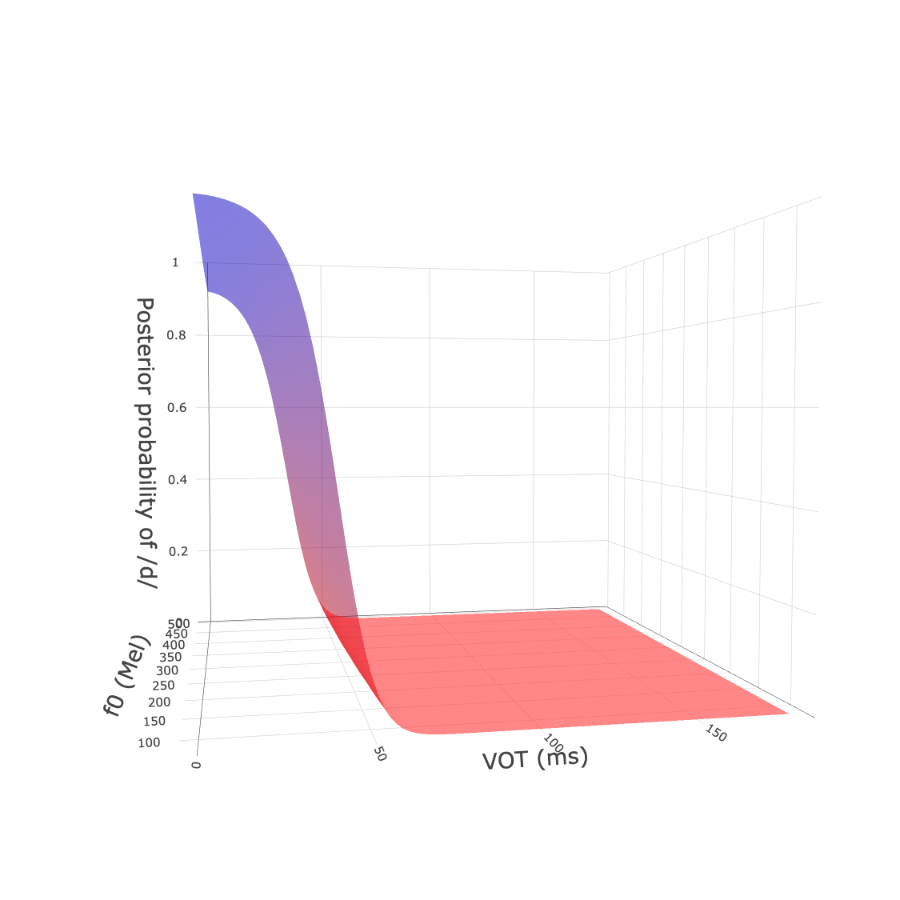
\includegraphics[width=0.33\linewidth,height=0.49\textheight]{../figures/plotly//p.3d.categorization.model_Representations_L1-accented} }\subfloat[Decision making: L1-accented\label{fig:show-model-categorization-3D-plots-2}]{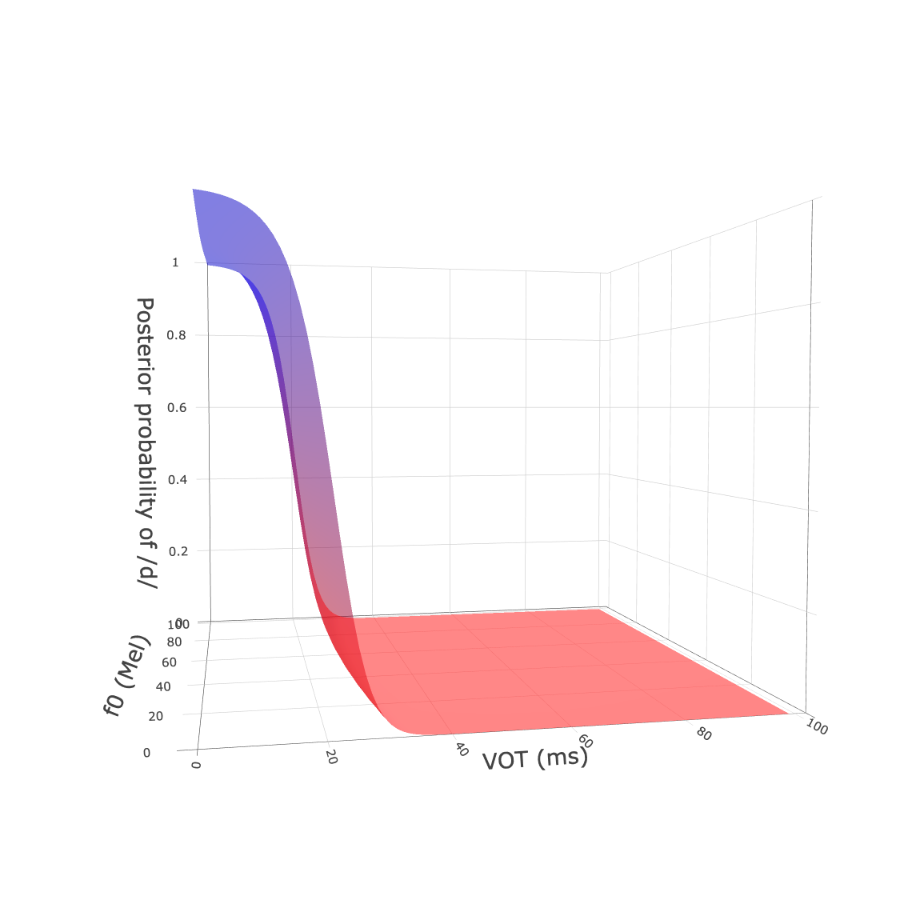
\includegraphics[width=0.33\linewidth,height=0.49\textheight]{../figures/plotly//p.3d.categorization.model_Decision_making_L1-accented} }\subfloat[Normalization: L1-accented\label{fig:show-model-categorization-3D-plots-3}]{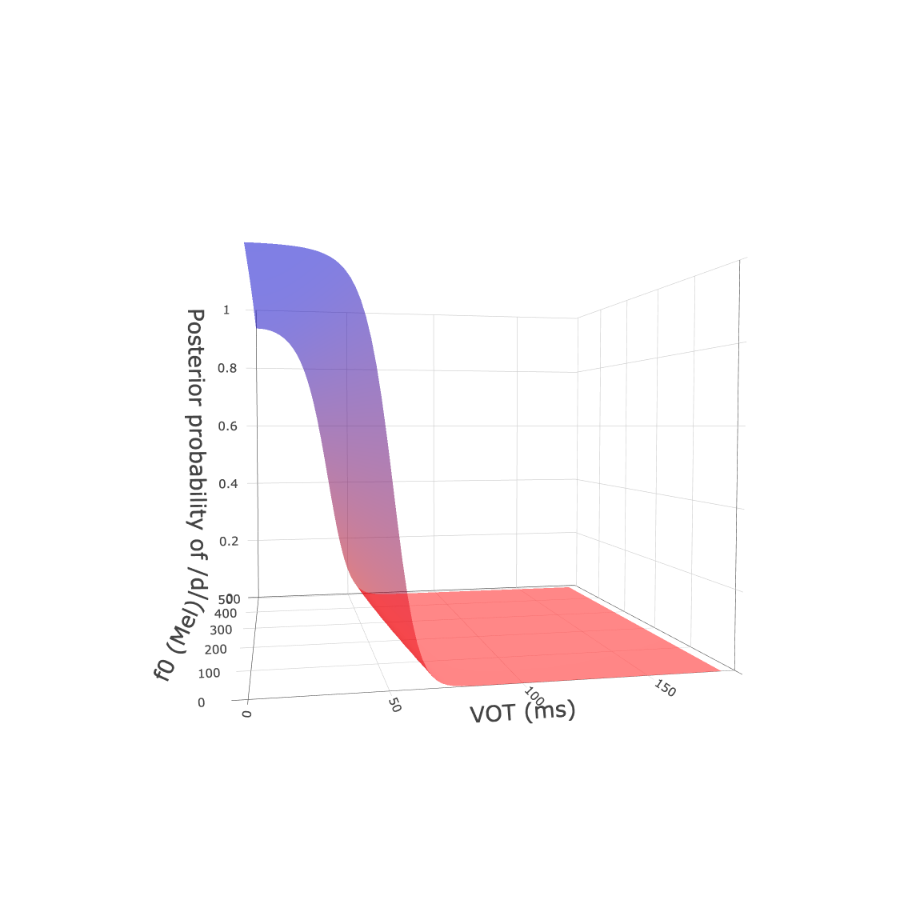
\includegraphics[width=0.33\linewidth,height=0.49\textheight]{../figures/plotly//p.3d.categorization.model_Normalization_L1-accented} }\newline\subfloat[Representations: L2-accented\label{fig:show-model-categorization-3D-plots-4}]{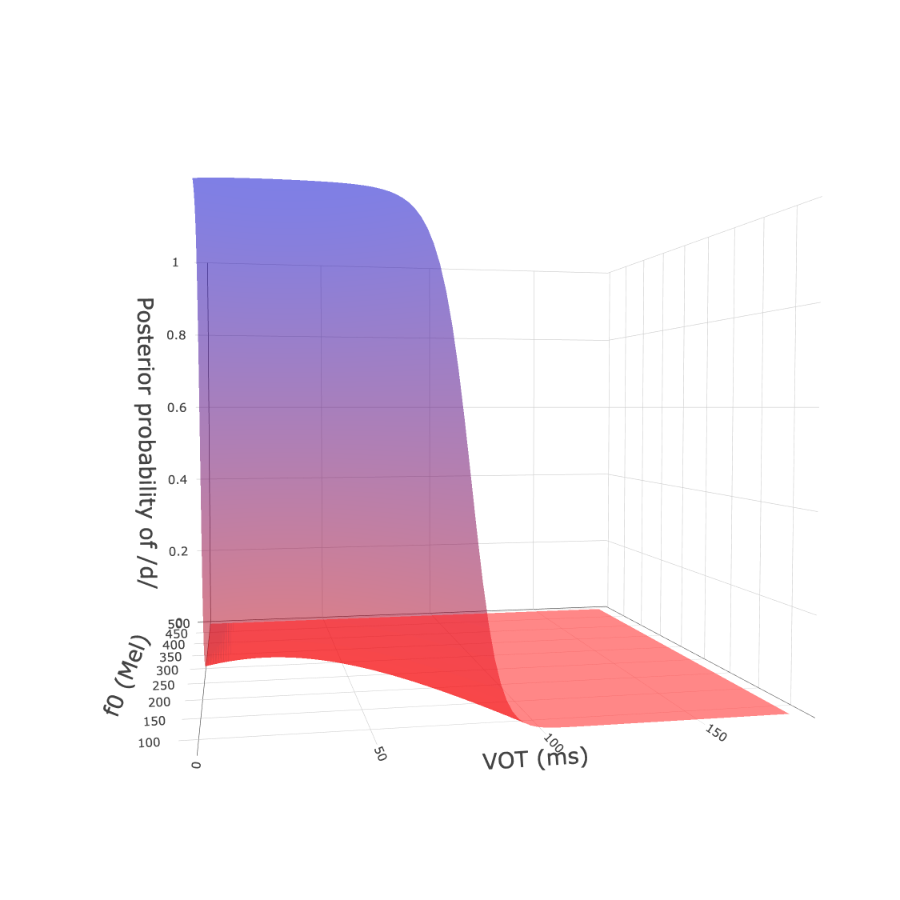
\includegraphics[width=0.33\linewidth,height=0.49\textheight]{../figures/plotly//p.3d.categorization.model_Representations_L2-accented} }\subfloat[Decision making: L2-accented\label{fig:show-model-categorization-3D-plots-5}]{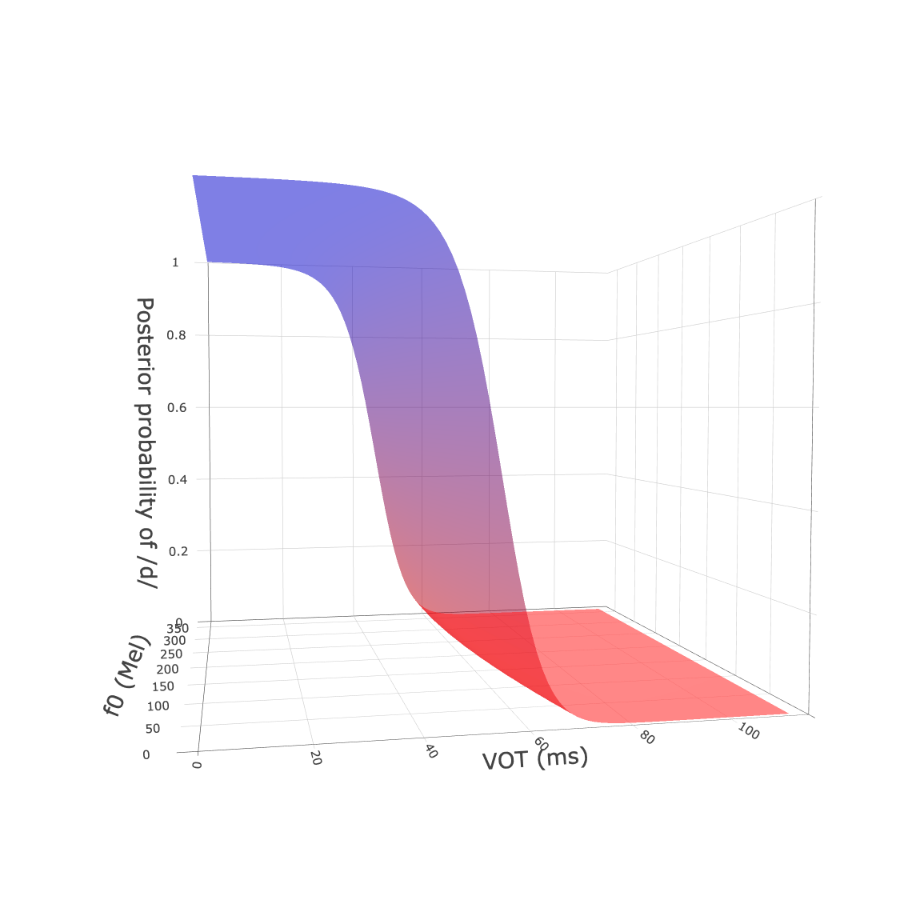
\includegraphics[width=0.33\linewidth,height=0.49\textheight]{../figures/plotly//p.3d.categorization.model_Decision_making_L2-accented} }\subfloat[Normalization: L2-accented\label{fig:show-model-categorization-3D-plots-6}]{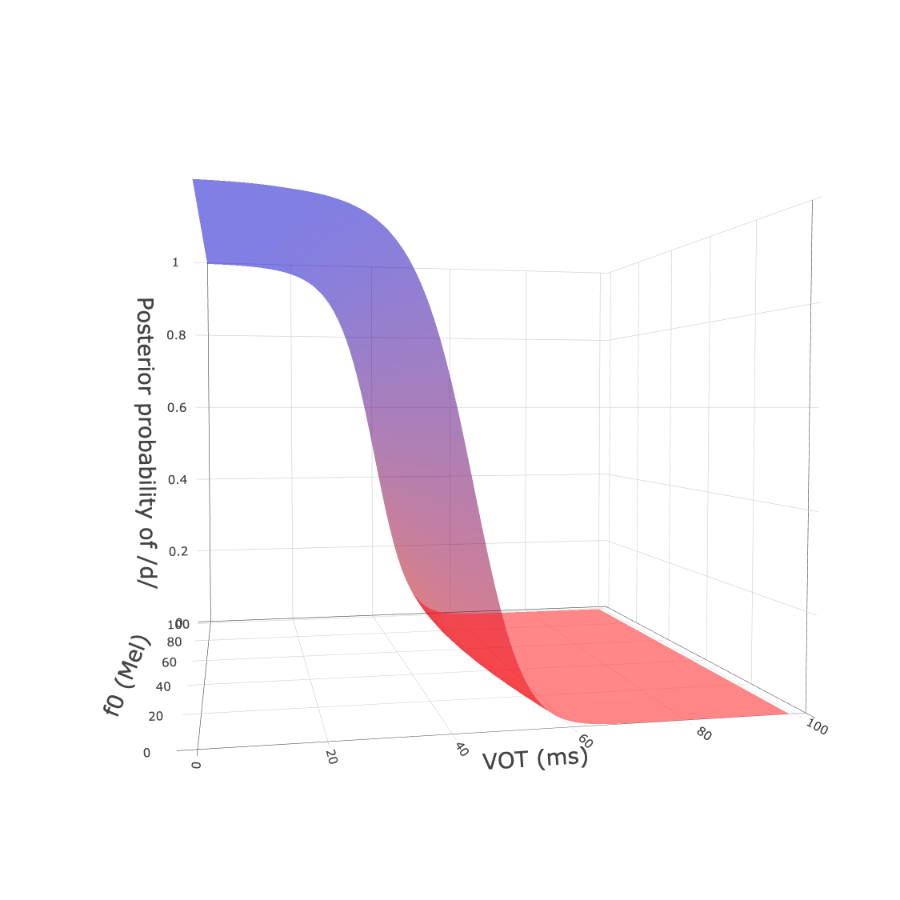
\includegraphics[width=0.33\linewidth,height=0.49\textheight]{../figures/plotly//p.3d.categorization.model_Normalization_L2-accented} }\newline\subfloat[Representations: difference\label{fig:show-model-categorization-3D-plots-7}]{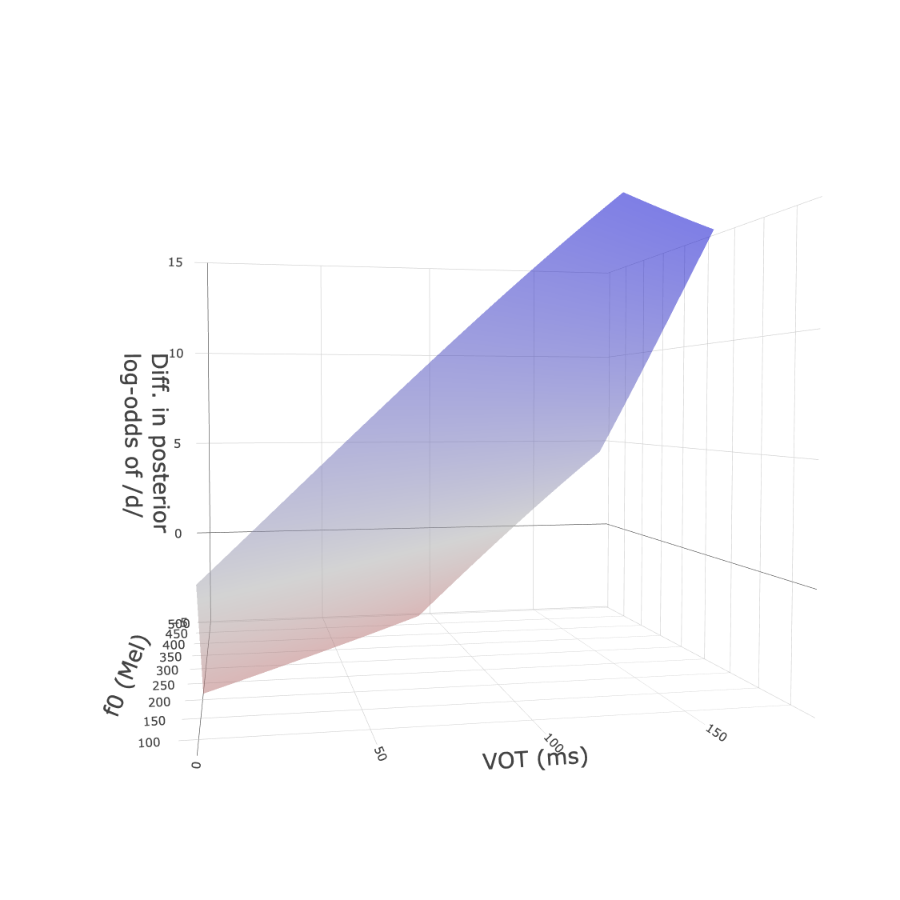
\includegraphics[width=0.33\linewidth,height=0.49\textheight]{../figures/plotly//p.3d.categorization.difference.model_Representations} }\subfloat[Decision making: difference\label{fig:show-model-categorization-3D-plots-8}]{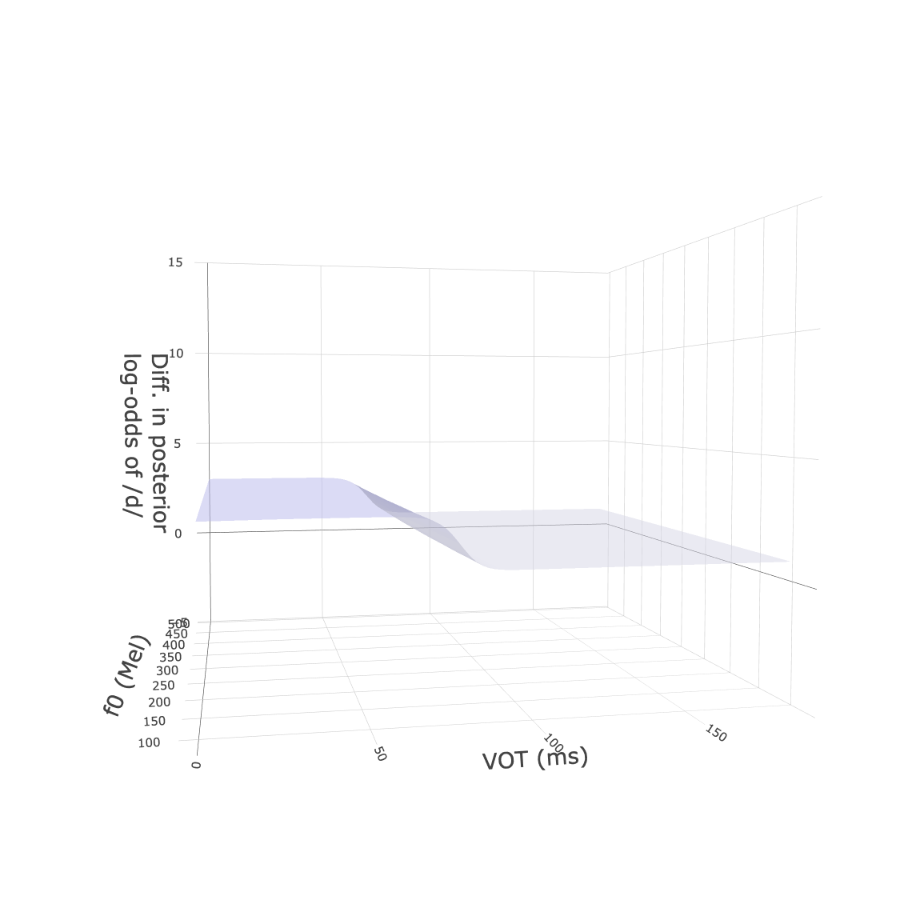
\includegraphics[width=0.33\linewidth,height=0.49\textheight]{../figures/plotly//p.3d.categorization.difference.model_Decision_making} }\subfloat[Normalization: difference\label{fig:show-model-categorization-3D-plots-9}]{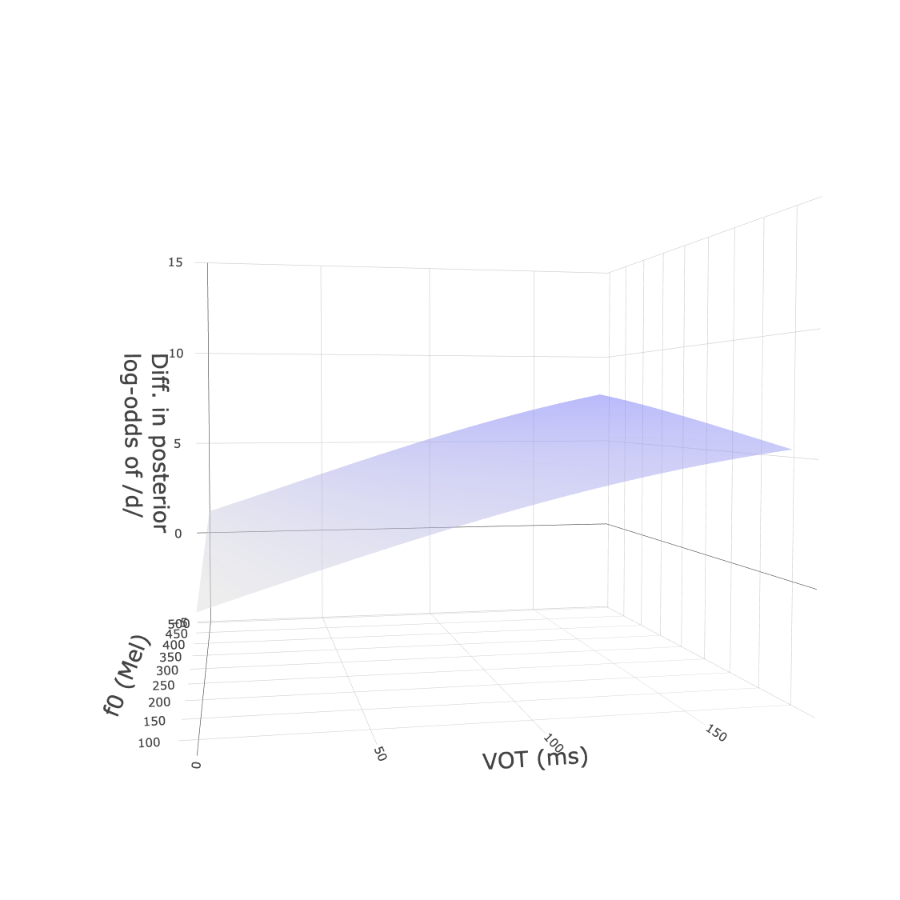
\includegraphics[width=0.33\linewidth,height=0.49\textheight]{../figures/plotly//p.3d.categorization.difference.model_Normalization} }

}

\caption{The three change models predict different categorization functions when applied to the data from Case Study 2. From \textbf{left to right:} predictions for in changes in representations, decision making, and normalization. \textbf{Top:} Predicted categorization functions after L1-accented exposure. \textbf{Middle:} Same but after L2-accented exposure. \textbf{Bottom:} Differences in predicted posterior log-odds of /d/ between the two exposure conditions. Blue indicates higher predicted posterior log-odds of /d/ in the L2-accented exposure condition, relative to the L1-accented exposure condition. Red indicates the opposite. Gray indicates a difference of 0. The three models make distinct predictions about how exposure affects the perception of specific tokens across the VOT-f0 space.}\label{fig:show-model-categorization-3D-plots}
\end{figure}

This points the way to approaches that can more clearly distinguish between the three competing mechanisms. Intuitively, paradigms and analyses should take advantage of the `richness' of the data. Most immediately, this is achieved by moving beyond comparisons that are limited to changes in overall categorization accuracy or processing speed, towards analyses that directly assess the link between the acoustic/phonetic properties of the speech input and listeners' responses. Such approaches are now increasingly common (e.g., \protect\hyperlink{ref-clare2019}{Clare, 2019}; \protect\hyperlink{ref-idemaru-holt2020}{Idemaru \& Holt, 2020}; \protect\hyperlink{ref-kartushina2015}{Kartushina et al., 2015}; \protect\hyperlink{ref-kim2020}{D. Kim et al., 2020}; \protect\hyperlink{ref-liu-holt2015}{R. Liu \& Holt, 2015}; \protect\hyperlink{ref-schertz2015}{Schertz et al., 2015}; \protect\hyperlink{ref-wade2007}{Wade et al., 2007}). In order to reliably detect changes in categorization functions, it can be beneficial to more densely sample the acoustic/phonetic space during the test phase. Strategic placement of test stimuli can be used to increase the statistical power to test predicted differences between the different change models (\protect\hyperlink{ref-burchill-jaeger2022}{Burchill \& Jaeger, 2021}). For example, the bottom row of Figure \ref{fig:show-model-categorization-3D-plots} suggests that denser sampling of certain VOT-f0 combinations should make it possible to distinguish between the three change models.

Moving beyond simple contrasts between two exposure conditions can further facilitate comparison between change models. The more exposure conditions an experiment employs, the more accurately and reliably the parameters of the competing change models can be estimated, increasing the power of the model comparison. For instance, Kleinschmidt and Jaeger (\protect\hyperlink{ref-kleinschmidt-jaeger2016cogsci}{2016b}) and Kleinschmidt (\protect\hyperlink{ref-kleinschmidt2020}{2020}) created six different between-subject exposure conditions with distinct distributions of VOT. By examining the degree of adaptive changes listeners exhibited in these six conditions, the researchers could estimate their prior expectations more reliably than when only one exposure condition is employed (see also \protect\hyperlink{ref-babel2019}{Babel et al., 2019}; \protect\hyperlink{ref-sumner2011}{Sumner, 2011}). Similarly, incremental testing \emph{within} subjects can increase statistical power to contrast the predictions of different change models. Even when all three change models predict the same \emph{outcome} of adaptation, they can differ in the trajectory of changes they predict. While incremental testing paradigms exist (e.g., \protect\hyperlink{ref-bertelson2003}{Bertelson et al., 2003}; \protect\hyperlink{ref-bonte2017}{Bonte et al., 2017}; \protect\hyperlink{ref-vroomen2007}{Vroomen et al., 2007}), they remain under-utilized, and model comparisons based on such experiments remain lacking (but see \protect\hyperlink{ref-kleinschmidt-jaeger2012}{Kleinschmidt \& Jaeger, 2012}).

Either approach---denser sampling of exposure conditions or denser sampling of test tokens---is not limited to paradigms that employ synthesized or otherwise manipulated stimuli (e.g., perceptual recalibration or standard distributional learning paradigms). For example, Chodroff and Wilson (\protect\hyperlink{ref-chodroff-wilson2020}{2020}) took advantage of naturally occurring variability, and created different exposure conditions by selecting different subsets of natural stimuli. This approach strikes a particularly intriguing balance between ecological validity and experimental control.

Finally, comparison across exposure and test conditions might also be achieved through meta-analyses. For example, an ongoing project in our labs pursues this latter approach by constructing a database of over 100,000 categorization responses from dozens of perceptual recalibration experiments on the English /s/-/\ipatext{ʃ}/ contrast. Each of these experiments employs slightly different exposure and test stimuli, potentially increasing the statistical power to distinguish between the competing models. Such item-level meta-analyses benefit immensely from open science standards that facilitate (or even require) the sharing of data in well-documented formats.

\hypertarget{data-analysis-beyond-overall-accuracy-and-speed}{%
\subsubsection{Data analysis beyond overall accuracy and speed}\label{data-analysis-beyond-overall-accuracy-and-speed}}

To take advantage of the richer types of data described in the previous section, it is also necessary to move towards analyses that go beyond changes in the overall accuracy or speed of comprehension. In particular, analyses that directly link relevant acoustic or phonetic properties of the input to listeners' responses strike us as promising. This should take into account that listeners rely on a multitude of cues (e.g., \protect\hyperlink{ref-mcmurray-jongman2011}{McMurray \& Jongman, 2011}) even when the experiment manipulates only one of them. Such analyses could employ the type of model we have described in this study. Alternatively, even simple regression can suffice as long as it employs appropriate linking functions (e.g., logistic regression for categorization, \protect\hyperlink{ref-agresti2019}{Agresti, 2019}; \protect\hyperlink{ref-jaeger2008}{Jaeger, 2008}). This approach is now increasingly common, taking advantage of stimulus-level variability within and across conditions to test hypotheses. These regression analyses can be expanded to accommodate lapse rates and response biases (e.g., \protect\hyperlink{ref-clayards2008}{Clayards et al., 2008}; \protect\hyperlink{ref-kleinschmidt2020}{Kleinschmidt, 2020}), and can be fit in standard statistics software (e.g., through \texttt{brms} \protect\hyperlink{ref-burkner2017}{Bürkner, 2017a} or other libraries in \texttt{R}). A comprehensive introduction to such models is provided in Wichmann and Hill (\protect\hyperlink{ref-wichmann-hill2001}{2001}).

Indeed, there are direct connections between the model we have employed here and lapsing logistic regression. For example, two Gaussian categories along a phonetic continuum result in linear effect of the continuum on the posterior log-odds of the categories if the two categories have identical variance, but linear + quadratic if the two categories have unequal variance (e.g., \protect\hyperlink{ref-kleinschmidt-jaeger2015}{Kleinschmidt \& Jaeger, 2015}; \protect\hyperlink{ref-kronrod2016}{Kronrod et al., 2016}). This prediction can only be appreciated if logistic regression is employed for the analysis of 2AFC categorization tasks, rather than ANOVA or similar methods. Schertz and Clare (\protect\hyperlink{ref-schertz-clare2020}{2020}) provides an excellent overview of how standard regression analyses can be---and have been---used to assess the effects multiple phonetic cues on listeners' responses.

\hypertarget{advance-standards-of-data-annotation-reporting-and-sharing}{%
\subsubsection{Advance standards of data annotation, reporting, and sharing}\label{advance-standards-of-data-annotation-reporting-and-sharing}}

Theories of speech perception now agree that the distribution of acoustic or phonetic cues in the input is critical to understanding speech perception. As described above, a deeper understanding of how recent exposure comes to shape speech perception requires that researchers acknowledge this link, and advance their standards of data reporting accordingly. We recommend that it should become standard for studies on speech perception to report the relevant phonetic properties of their stimuli. For the paradigms like the ones we have discussed here, this would include phonetic annotations of both the exposure and test stimuli. As an added benefit, phonetic annotations also allow more sophisticated and natural stimulus manipulation (see the insightful critique offered in \protect\hyperlink{ref-theodore2021}{Theodore, 2021}).

In our view, such annotations entail a manageable effort: perception experiments typically employ a small number of speech stimuli that are repeated for each participant. A typical perceptual recalibration experiment would require the annotation of less than 100 isolated word recordings. A large study on accent adaptation like Bradlow and Bent's (2008) Experiment 2 would require the annotation of about 1000 sentences. Studies on phonetic production regularly annotate data sets many times larger. These efforts towards a more open, collaborative science can further be supported by clear standards for reproducibility and software developments that aid phonetic annotation and data sharing (e.g., \protect\hyperlink{ref-cassidy-schmidt2017}{Cassidy \& Schmidt, 2017}; \protect\hyperlink{ref-picoral2021}{Picoral, Staples, \& Reppen, 2021}; \protect\hyperlink{ref-roettger2019}{Roettger, Winter, \& Baayen, 2019}; \protect\hyperlink{ref-winkelmann2017}{Winkelmann, Harrington, \& Jänsch, 2017}). If annotations are not reported and shared---and ideally even if they are---then all audio recordings should be shared in an open and accessible way (e.g., OSF). This will require perception researchers to elicit recordings in ways that gives them the consent to distribute these recordings for the purpose of scientific inquiry. In other words, perception researchers would have to follow the same standards that researchers working on language production are expected to follow.

\hypertarget{simulation-and-power-analysis-prior-to-conducting-testing}{%
\subsubsection{Simulation and power analysis prior to conducting testing}\label{simulation-and-power-analysis-prior-to-conducting-testing}}

As detailed above, it is critical to formulate clear linking hypotheses that describe the mapping from the acoustic/phonetic input to perception (see also \protect\hyperlink{ref-apfelbaum-mcmurray2015}{Apfelbaum \& McMurray, 2015}; \protect\hyperlink{ref-tanenhaus2004}{Tanenhaus, 2004}). Analytical frameworks like the one we introduced here can be used to estimate expected sizes of effects before conducting an experiment. Unlike commonly used power estimates---which assume expected effect sizes (based on previous work or arbitrarily set to e.g., ``moderate'')---a fully specified change model can derive predicted effect sizes under a hypothesized mechanism. This will make power-analyses less arbitrary and more informative.

In addition to phonetically annotated exposure and test stimuli, such power analyses require estimates of listeners' prior expectations at the start of the experiment. Because these estimates aim to capture expectations based on input previously experienced throughout listeners' lives, these estimates entail substantially more effort than the annotation of experimental stimuli. Fortunately, large and phonetically annotated databases of the speech variety assumed to have been the primary input of the listeners under study. Such databases are now available for an increasing number of phonological contrasts and languages (e.g., \protect\hyperlink{ref-chodroff-wilson2018}{Chodroff \& Wilson, 2018}; \protect\hyperlink{ref-clopper-pisoni2006}{Clopper \& Pisoni, 2006}; \protect\hyperlink{ref-hillenbrand1995}{Hillenbrand, Getty, Clark, \& Wheeler, 1995}; \protect\hyperlink{ref-newman2001}{Newman et al., 2001}; \protect\hyperlink{ref-theodore2009}{Theodore, Miller, \& DeSteno, 2009}; \protect\hyperlink{ref-xie-jaeger2020}{X. Xie \& Jaeger, 2020}, among many others). One caveat is that many of these databases either are representative only of a subset of the varieties that an average speaker of a language has plausibly been exposed to, or contain very little data for each variety. In particular, databases that contain both a large number of talkers, and a large number of tokens per talker, continue to be the exception. Researchers need to carefully consider these implications when employing databases. In some cases, researchers might find that the best way forward is to collect phonetically annotated data that meets the specific requirements for their study. X. Xie, Buxó-Lugo, et al. (\protect\hyperlink{ref-xie2021cognition}{2021}), for instance, collected \textasciitilde3000 production tokens of prosodic categories and used them to model listeners' responses in a perception experiment. We have also found that sometimes phonetically annotated data from a single typical talker can be sufficient to get started---e.g., to gain an initial understanding of one's results (\protect\hyperlink{ref-tan2021}{Tan et al., 2021}) or to conduct power simulations.

One alternative option is to eschew phonetically annotated data in favor of computational methods that work with the raw signal or some automatically obtained transformation of the raw data (such as Mel-Frequency Cepstral Coefficents, (MFCC) \protect\hyperlink{ref-Mermelstein1976}{Mermelstein, 1976}). Such models have been developed for automatic speech recognition (for an earlier review, see \protect\hyperlink{ref-jurafsky-martin2000}{Jurafsky \& Martin, 2000}) and have been employed to model human language acquisition (\protect\hyperlink{ref-dupoux2018}{Dupoux, 2018}; \protect\hyperlink{ref-feldman2013}{Feldman, Myers, White, Griffiths, \& Morgan, 2013}; \protect\hyperlink{ref-toscano-mcmurray2010}{Toscano \& McMurray, 2010}; \protect\hyperlink{ref-vallabha2007}{Vallabha, McClelland, Pons, Werker, \& Amano, 2007}). More recently, they have also been applied to address questions about the effects of recent exposure (\protect\hyperlink{ref-richter2017}{Richter et al., 2017}). The general framework we have described here can be combined with such models.

\begin{quote}
There is no real ending. It's just the place where you stop the story.

\hfill --- Frank Herbert
\end{quote}

\newpage

\hypertarget{references}{%
\section{References}\label{references}}

\begingroup
\setlength{\parindent}{-0.5in}
\setlength{\leftskip}{0.5in}

\hypertarget{refs}{}
\begin{CSLReferences}{1}{0}
\leavevmode\vadjust pre{\hypertarget{ref-adank2009}{}}%
Adank, P., Evans, B. G., Stuart-Smith, J., \& Scott, S. K. (2009). Comprehension of familiar and unfamiliar native accents under adverse listening conditions. \emph{Journal of Experimental Psychology: Human Perception and Performance}, \emph{35}, 520. \url{https://doi.org/10.1037/a0013552}

\leavevmode\vadjust pre{\hypertarget{ref-adank2004}{}}%
Adank, P., Smits, R., \& Hout, R. van. (2004). A comparison of vowel normalization procedures for language variation research. \emph{The Journal of the Acoustical Society of America}, \emph{116}, 3099--3107. \url{https://doi.org/10.1121/1.1795335}

\leavevmode\vadjust pre{\hypertarget{ref-agresti2019}{}}%
Agresti, A. (2019). \emph{An introduction to categorical data analysis / alan agresti, university of florida, florida, united states.} (Third edition.). Hoboken, NJ: Wiley.

\leavevmode\vadjust pre{\hypertarget{ref-apfelbaum-mcmurray2015}{}}%
Apfelbaum, K., \& McMurray, B. (2015). Relative cue encoding in the context of sophisticated models of categorization: Separating information from categorization. \emph{Psychonomic Bulletin and Review}, \emph{22}, 916--943. \url{https://doi.org/10.3758/s13423-014-0783-2}

\leavevmode\vadjust pre{\hypertarget{ref-R-papaja}{}}%
Aust, F., \& Barth, M. (2020). \emph{{papaja}: {Create} {APA} manuscripts with {R Markdown}}. Retrieved from \url{https://github.com/crsh/papaja}

\leavevmode\vadjust pre{\hypertarget{ref-baart-vroomen2010}{}}%
Baart, M., \& Vroomen, J. (2010). Phonetic recalibration does not depend on working memory. \emph{Experimental Brain Research}, \emph{203}, 575--582. \url{https://doi.org/10.1007/s00221-010-2264-9}

\leavevmode\vadjust pre{\hypertarget{ref-babel2019}{}}%
Babel, M., Senior, B., \& Bishop, S. (2019). Do social preferences matter in lexical retuning? \emph{Laboratory Phonology: Journal of the Association for Laboratory Phonology}, \emph{10}. \url{https://doi.org/10.5334/labphon.133}

\leavevmode\vadjust pre{\hypertarget{ref-R-magrittr}{}}%
Bache, S. M., \& Wickham, H. (2020). \emph{Magrittr: A forward-pipe operator for r}. Retrieved from \url{https://CRAN.R-project.org/package=magrittr}

\leavevmode\vadjust pre{\hypertarget{ref-baeseberk2013}{}}%
Baese-Berk, M. M., Bradlow, A. R., \& Wright, B. A. (2013). Accent-independent adaptation to foreign accented speech. \emph{The Journal of the Acoustical Society of America}, \emph{133}, 174--180.

\leavevmode\vadjust pre{\hypertarget{ref-baeseberk2020}{}}%
Baese-Berk, M. M., McLaughlin, D. J., \& McGowan, K. B. (2020). Perception of non-native speech. \emph{Language and Linguistics Compass}, \emph{14}, 1--20. \url{https://doi.org/10.1111/lnc3.12375}

\leavevmode\vadjust pre{\hypertarget{ref-baeseberk2018}{}}%
Baese-Berk, M. M., Walker, K., \& Bradlow, A. (2018). Variability in speaking rate of native and non-native speakers. \emph{The Journal of the Acoustical Society of America}, \emph{144}, 1717--1717. \url{https://doi.org/10.1121/1.5067612}

\leavevmode\vadjust pre{\hypertarget{ref-barreda2012}{}}%
Barreda, S. (2012). Vowel normalization and the perception of speaker changes: An exploration of the contextual tuning hypothesis. \emph{The Journal of the Acoustical Society of America}, \emph{132}, 3453--3464. \url{https://doi.org/10.1121/1.4747011}

\leavevmode\vadjust pre{\hypertarget{ref-R-tinylabels}{}}%
Barth, M. (2022). \emph{{tinylabels}: Lightweight variable labels}. Retrieved from \url{https://cran.r-project.org/package=tinylabels}

\leavevmode\vadjust pre{\hypertarget{ref-R-lme4}{}}%
Bates, D., Mächler, M., Bolker, B., \& Walker, S. (2015). Fitting linear mixed-effects models using {lme4}. \emph{Journal of Statistical Software}, \emph{67}(1), 1--48. \url{https://doi.org/10.18637/jss.v067.i01}

\leavevmode\vadjust pre{\hypertarget{ref-R-Matrix}{}}%
Bates, D., \& Maechler, M. (2021). \emph{Matrix: Sparse and dense matrix classes and methods}. Retrieved from \url{https://CRAN.R-project.org/package=Matrix}

\leavevmode\vadjust pre{\hypertarget{ref-bejjanki2011}{}}%
Bejjanki, V. R., Clayards, M., Knill, D. C., \& Aslin, R. N. (2011). Cue integration in categorical tasks: Insights from audio-visual speech perception. \emph{PLoS ONE}, \emph{6}, 1--12.

\leavevmode\vadjust pre{\hypertarget{ref-bent-baeseberk2021}{}}%
Bent, T., \& Baese-Berk, M. M. (2021). Perceptual learning of accented speech. \emph{The Handbook of Speech Perception}, 428--464. \url{https://doi.org/10.1002/9781119184096.ch16}

\leavevmode\vadjust pre{\hypertarget{ref-bertelson2003}{}}%
Bertelson, P., Vroomen, J., \& Gelder, B. de. (2003). Visual recalibration of auditory speech identification. \emph{Psychological Science}, \emph{14}, 592--597. \url{https://doi.org/10.1046/j.0956-7976.2003.psci_1470.x}

\leavevmode\vadjust pre{\hypertarget{ref-bieber2021}{}}%
Bieber, R. E., \& Gordon-Salant, S. (2021). Improving older adults' understanding of challenging speech: Auditory training, rapid adaptation and perceptual learning. \emph{Hearing Research}, \emph{402}, 108054. \url{https://doi.org/10.1016/j.heares.2020.108054}

\leavevmode\vadjust pre{\hypertarget{ref-binder2004neural}{}}%
Binder, J. R., Liebenthal, E., Possing, E. T., Medler, D. A., \& Ward, B. D. (2004). Neural correlates of sensory and decision processes in auditory object identification. \emph{Nature Neuroscience}, \emph{7}(3), 295--301.

\leavevmode\vadjust pre{\hypertarget{ref-blanco-elorriera2021}{}}%
Blanco-Elorrieta, E., Gwilliams, L., Marantz, A., \& Pylkkänen, L. (2021). Adaptation to mis-pronounced speech: Evidence for a prefrontal-cortex repair mechanism. \emph{Scientific Reports}, \emph{11}. \url{https://doi.org/10.1038/s41598-020-79640-0}

\leavevmode\vadjust pre{\hypertarget{ref-bonte2017}{}}%
Bonte, M., Correia, J. M., Keetels, M., Vroomen, J., \& Formisano, E. (2017). Reading-induced shifts of perceptual speech representations in auditory cortex. \emph{Scientific Reports}, \emph{7}, 5143. \url{https://doi.org/10.1038/s41598-017-05356-3}

\leavevmode\vadjust pre{\hypertarget{ref-bosch2015}{}}%
Bosch, L. ten, Boves, L., Tucker, B., \& Ernestus, M. (2015). \emph{DIANA: Towards computational modeling reaction times in lexical decision in north american english}. 1576--1580. \url{https://doi.org/10.21437/Interspeech.2015-366}

\leavevmode\vadjust pre{\hypertarget{ref-bosker2017}{}}%
Bosker, H. R., Reinisch, E., \& Sjerps, M. J. (2017). Cognitive load makes speech sound fast, but does not modulate acoustic context effects. \emph{Journal of Memory and Language}, \emph{94}, 166--176. https://doi.org/\url{https://doi.org/10.1016/j.jml.2016.12.002}

\leavevmode\vadjust pre{\hypertarget{ref-bradlow-bent2008}{}}%
Bradlow, A. R., \& Bent, T. (2008). Perceptual adaptation to non-native speech. \emph{Cognition}, \emph{106}, 707--729.

\leavevmode\vadjust pre{\hypertarget{ref-burchill-jaeger2022}{}}%
Burchill, Z., \& Jaeger, T. F. (2021). \href{}{A manuscript under revision}. \emph{XXXX}.

\leavevmode\vadjust pre{\hypertarget{ref-burkner2017}{}}%
Bürkner, P.-C. (2017a). \emph{Advanced bayesian multilevel modeling with the r package brms}. Retrieved from \url{https://arxiv.org/abs/1705.11123}

\leavevmode\vadjust pre{\hypertarget{ref-R-brms_a}{}}%
Bürkner, P.-C. (2017b). {brms}: An {R} package for {Bayesian} multilevel models using {Stan}. \emph{Journal of Statistical Software}, \emph{80}(1), 1--28. \url{https://doi.org/10.18637/jss.v080.i01}

\leavevmode\vadjust pre{\hypertarget{ref-R-brms_b}{}}%
Bürkner, P.-C. (2018). Advanced {Bayesian} multilevel modeling with the {R} package {brms}. \emph{The R Journal}, \emph{10}(1), 395--411. \url{https://doi.org/10.32614/RJ-2018-017}

\leavevmode\vadjust pre{\hypertarget{ref-R-brms_c}{}}%
Bürkner, P.-C. (2021). Bayesian item response modeling in {R} with {brms} and {Stan}. \emph{Journal of Statistical Software}, \emph{100}(5), 1--54. \url{https://doi.org/10.18637/jss.v100.i05}

\leavevmode\vadjust pre{\hypertarget{ref-carlisle1991}{}}%
Carlisle, R. S. (1991). {The Influence of Environment on Vowel Epenthesis in Spanish/English Interphonology}. \emph{Applied Linguistics}, \emph{12}(1), 76--95. \url{https://doi.org/10.1093/applin/12.1.76}

\leavevmode\vadjust pre{\hypertarget{ref-cassidy-schmidt2017}{}}%
Cassidy, S., \& Schmidt, T. (2017). Tools for multimodal annotation. \emph{Handbook of Linguistic Annotation}, 209--227. \url{https://doi.org/10.1007/978-94-024-0881-2_7}

\leavevmode\vadjust pre{\hypertarget{ref-chodroff-wilson2018}{}}%
Chodroff, E., \& Wilson, C. (2018). Predictability of stop consonant phonetics across talkers: Between-category and within-category dependencies among cues for place and voice. \emph{Linguistics Vanguard}, \emph{4}. \url{https://doi.org/10.1515/lingvan-2017-0047}

\leavevmode\vadjust pre{\hypertarget{ref-chodroff-wilson2020}{}}%
Chodroff, E., \& Wilson, C. (2020). Acoustic--phonetic and auditory mechanisms of adaptation in the perception of sibilant fricatives. \emph{Attention, Perception, and Psychophysics}, \emph{82}, 2027--2048. \url{https://doi.org/10.3758/s13414-019-01894-2}

\leavevmode\vadjust pre{\hypertarget{ref-clare2019}{}}%
Clare, E. (2019). \emph{Dynamicity in speech perception}. University of Toronto.

\leavevmode\vadjust pre{\hypertarget{ref-clark2013}{}}%
Clark, A. (2013). Whatever next? Predictive brains, situated agents, and the future of cognitive science. \emph{The Behavioral and Brain Sciences}, \emph{36}, 181--204. \url{https://doi.org/10.1017/S0140525X12000477}

\leavevmode\vadjust pre{\hypertarget{ref-clarke-garrett2004}{}}%
Clarke, C. M., \& Garrett, M. F. (2004). Rapid adaptation to foreign-accented english. \emph{The Journal of the Acoustical Society of America}, \emph{116}, 3647. \url{https://doi.org/10.1121/1.1815131}

\leavevmode\vadjust pre{\hypertarget{ref-clarkedavidson2008}{}}%
Clarke-Davidson, C. M., Luce, P. A., \& Sawusch, J. R. (2008). Does perceptual learning in speech reflect changes in phonetic category representation or decision bias ? \emph{Perception \& Psychophysics}, \emph{70}, 604--618. \url{https://doi.org/10.3758/PP.70.4.604}

\leavevmode\vadjust pre{\hypertarget{ref-clayards2008}{}}%
Clayards, M., Tanenhaus, M. K., Aslin, R. N., \& Jacobs, R. A. (2008). Perception of speech reflects optimal use of probabilistic speech cues. \emph{Cognition}, \emph{108}, 804--809. \url{https://doi.org/10.1016/j.cognition.2008.04.004}

\leavevmode\vadjust pre{\hypertarget{ref-clopper-bradlow2008}{}}%
Clopper, C. G., \& Bradlow, A. R. (2008). Perception of dialect variation in noise: Intelligibility and classification. \emph{Language and Speech}, \emph{51}, 175--198. \url{https://doi.org/10.1177/0023830908098539}

\leavevmode\vadjust pre{\hypertarget{ref-clopper-pisoni2006}{}}%
Clopper, C. G., \& Pisoni, D. B. (2006). The nationwide speech project: A new corpus of american english dialects. \emph{Speech Communication}, \emph{48}, 633--644. \url{https://doi.org/10.1016/j.specom.2005.09.010}

\leavevmode\vadjust pre{\hypertarget{ref-cole2010}{}}%
Cole, J., Linebaugh, G., Munson, C., \& McMurray, B. (2010). Unmasking the acoustic effects of vowel-to-vowel coarticulation: A statistical modeling approach. \emph{Journal of Phonetics}, \emph{38}, 167--184. \url{https://doi.org/10.1016/j.wocn.2009.08.004}

\leavevmode\vadjust pre{\hypertarget{ref-contemori-tortajada2020}{}}%
Contemori, C., \& Tortajada, F. (2020). The use of social-communicative cues to interpret ambiguous pronouns: Bilingual adults differ from monolinguals. \emph{Applied Psycholinguistics}, \emph{41}, 51--77. \url{https://doi.org/10.1017/S0142716419000407}

\leavevmode\vadjust pre{\hypertarget{ref-cooper-bradlow2016}{}}%
Cooper, A., \& Bradlow, A. R. (2016). Linguistically guided adaptation to foreign-accented speech. \emph{The Journal of the Acoustical Society of America}, \emph{140}, EL378--EL384. \url{https://doi.org/10.1121/1.4966585}

\leavevmode\vadjust pre{\hypertarget{ref-creel-bregman2011}{}}%
Creel, S. C., \& Bregman, M. R. (2011). \emph{How talker identity relates to language processing}. \emph{5}, 190--204.

\leavevmode\vadjust pre{\hypertarget{ref-R-processx}{}}%
Csárdi, G., \& Chang, W. (2021). \emph{Processx: Execute and control system processes}. Retrieved from \url{https://CRAN.R-project.org/package=processx}

\leavevmode\vadjust pre{\hypertarget{ref-cutler-jesse2021}{}}%
Cutler, A., \& Jesse, A. (2021). Word stress in speech perception. \emph{The Handbook of Speech Perception}, 239--265. \url{https://doi.org/10.1002/9781119184096.ch9}

\leavevmode\vadjust pre{\hypertarget{ref-dacremont2013}{}}%
d'Acremont, M., Schultz, W., \& Bossaerts, P. (2013). The human brain encodes event frequencies while forming subjective beliefs. \emph{Journal of Neuroscience}, \emph{33}, 10887--10897. \url{https://doi.org/10.1523/JNEUROSCI.5829-12.2013}

\leavevmode\vadjust pre{\hypertarget{ref-dahan2008}{}}%
Dahan, D., Drucker, S. J., \& Scarborough, R. A. (2008). Talker adaptation in speech perception: Adjusting the signal or the representations? \emph{Cognition}, \emph{108}, 710--718. \url{https://doi.org/10.1016/j.cognition.2008.06.003}

\leavevmode\vadjust pre{\hypertarget{ref-davis2005}{}}%
Davis, M. H., Johnsrude, I. S., Hervais-Adelman, A., Taylor, K., \& McGettigan, C. (2005). Lexical information drives perceptual learning of distorted speech: Evidence from the comprehension of noise-vocoded sentences. \emph{Journal of Experimental Psychology: General}, \emph{134}, 222--241. \url{https://doi.org/10.1037/0096-3445.134.2.222}

\leavevmode\vadjust pre{\hypertarget{ref-R-data.table}{}}%
Dowle, M., \& Srinivasan, A. (2021). \emph{Data.table: Extension of `data.frame`}. Retrieved from \url{https://CRAN.R-project.org/package=data.table}

\leavevmode\vadjust pre{\hypertarget{ref-drouin2016}{}}%
Drouin, J. R., Theodore, R., \& Myers, E. B. (2016). Lexically guided perceptual tuning of internal phonetic category structure. \emph{The Journal of the Acoustical Society of America}, \emph{140}(4), EL307--EL313. \url{https://doi.org/doi.org/10.1121/1.4964468}

\leavevmode\vadjust pre{\hypertarget{ref-dupoux2018}{}}%
Dupoux, E. (2018). Cognitive science in the era of artificial intelligence: A roadmap for reverse-engineering the infant language-learner. \emph{Cognition}, \emph{173}, 43--59. https://doi.org/\url{https://doi.org/10.1016/j.cognition.2017.11.008}

\leavevmode\vadjust pre{\hypertarget{ref-R-Rcpp_b}{}}%
Eddelbuettel, D., \& Balamuta, J. J. (2018). {Extending extit{R} with extit{C++}: A Brief Introduction to extit{Rcpp}}. \emph{The American Statistician}, \emph{72}(1), 28--36. \url{https://doi.org/10.1080/00031305.2017.1375990}

\leavevmode\vadjust pre{\hypertarget{ref-R-Rcpp_a}{}}%
Eddelbuettel, D., \& François, R. (2011). {Rcpp}: Seamless {R} and {C++} integration. \emph{Journal of Statistical Software}, \emph{40}(8), 1--18. \url{https://doi.org/10.18637/jss.v040.i08}

\leavevmode\vadjust pre{\hypertarget{ref-eisner-mcqueen2006}{}}%
Eisner, F., \& McQueen, J. M. (2006). Perceptual learning in speech: Stability over time. \emph{The Journal of the Acoustical Society of America}, \emph{119}, 1950--1953. \url{https://doi.org/10.1121/1.2178721}

\leavevmode\vadjust pre{\hypertarget{ref-eisner2013}{}}%
Eisner, F., Melinger, A., \& Weber, A. (2013). Constraints on the transfer of perceptual learning in accented speech. \emph{Frontiers in Psychology}, \emph{4}, 148. \url{https://doi.org/10.3389/fpsyg.2013.00148}

\leavevmode\vadjust pre{\hypertarget{ref-erb2013brain}{}}%
Erb, J., Henry, M. J., Eisner, F., \& Obleser, J. (2013). The brain dynamics of rapid perceptual adaptation to adverse listening conditions. \emph{Journal of Neuroscience}, \emph{33}(26), 10688--10697.

\leavevmode\vadjust pre{\hypertarget{ref-feldman2009}{}}%
Feldman, N. H., Griffiths, T. L., \& Morgan, J. L. (2009). The influence of categories on perception: Explaining the perceptual magnet effect as optimal statistical inference. \emph{Psychological Review}, \emph{116}, 752--782.

\leavevmode\vadjust pre{\hypertarget{ref-feldman2013}{}}%
Feldman, N. H., Myers, E. B., White, K. S., Griffiths, T. L., \& Morgan, J. L. (2013). Word-level information influences phonetic learning in adults and infants. \emph{Cognition}, \emph{127}, 427--438. https://doi.org/\url{https://doi.org/10.1016/j.cognition.2013.02.007}

\leavevmode\vadjust pre{\hypertarget{ref-fenn2003}{}}%
Fenn, K. M., Nusbaum, H. C., \& Margoliash, D. (2003). Consolidation during sleep of perceptual learning of spoken language. \emph{Letters to Nature}, \emph{425}, 614--616. \url{https://doi.org/10.1038/nature01971.1.}

\leavevmode\vadjust pre{\hypertarget{ref-fine-jaeger2013}{}}%
Fine, A. B., \& Jaeger, T. F. (2013). Evidence for implicit learning in syntactic comprehension. \emph{Cognitive Science}, \emph{37}, 578--591. \url{https://doi.org/doi:10.1111/cogs.12022}

\leavevmode\vadjust pre{\hypertarget{ref-fix-hodges1989}{}}%
Fix, E., \& Hodges, J. L. (1989). Discriminatory analysis - nonparametric discrimination: Consistency properties. \emph{International Statistical Review}, \emph{57}, 238--247.

\leavevmode\vadjust pre{\hypertarget{ref-flege1992}{}}%
Flege, J. E., Munro, M. J., \& Skelton, L. (1992). Production of the word‐final english /t/--/d/ contrast by native speakers of english, mandarin, and spanish. \emph{The Journal of the Acoustical Society of America}, \emph{92}, 128--143. \url{https://doi.org/10.1121/1.404278}

\leavevmode\vadjust pre{\hypertarget{ref-foulkes-hay2015}{}}%
Foulkes, P., \& Hay, J. B. (2015). The emergence of sociophonetic structure. \url{https://doi.org/doi:10.1002/9781118346136.ch13}

\leavevmode\vadjust pre{\hypertarget{ref-furl2011parietal}{}}%
Furl, N., \& Averbeck, B. B. (2011). Parietal cortex and insula relate to evidence seeking relevant to reward-related decisions. \emph{Journal of Neuroscience}, \emph{31}(48), 17572--17582.

\leavevmode\vadjust pre{\hypertarget{ref-ganong1980}{}}%
Ganong, W. F. (1980). Phonetic categorization in auditory word perception. \emph{Journal of Experimental Psychology: Human Perception and Performance}, \emph{6}, 110--125.

\leavevmode\vadjust pre{\hypertarget{ref-gerstman1968}{}}%
Gerstman, L. (1968). Classification of self-normalized vowels. \emph{IEEE Transactions on Audio and Electroacoustics}, \emph{16}(1), 78--80. \url{https://doi.org/10.1109/TAU.1968.1161953}

\leavevmode\vadjust pre{\hypertarget{ref-goldinger1996}{}}%
Goldinger, S. D. (1996). Words and voices: Episodic traces in spoken word identification and recognition memory. \emph{Journal of Experimental Psychology: Learning, Memory and Cognition}, \emph{22}, 1166--1183. \url{https://doi.org/10.1037/0278-7393.22.5.1166}

\leavevmode\vadjust pre{\hypertarget{ref-goldinger1998}{}}%
Goldinger, S. D. (1998). Echoes of echoes?: An episodic theory of lexical access. \emph{Psychological Review}, \emph{105}, 251--279.

\leavevmode\vadjust pre{\hypertarget{ref-goldinger-azuma2004}{}}%
Goldinger, S. D., \& Azuma, T. (2004). Episodic memory reflected in printed word naming. \emph{Psychonomic Bulletin and Review}, \emph{11}, 716--722.

\leavevmode\vadjust pre{\hypertarget{ref-gordonsalant2010}{}}%
Gordon-Salant, S., Yeni-Komshian, G. H., Fitzgibbons, P. J., \& Schurman, J. (2010). Short-term adaptation to accented english by younger and older adults. \emph{The Journal of the Acoustical Society of America}, \emph{128}, EL200--4. \url{https://doi.org/10.1121/1.3486199}

\leavevmode\vadjust pre{\hypertarget{ref-greenwood1961}{}}%
Greenwood, D. D. (1961). Auditory masking and the critical band. \emph{The Journal of the Acoustical Society of America}, \emph{33}, 484--502. \url{https://doi.org/10.1121/1.1908699}

\leavevmode\vadjust pre{\hypertarget{ref-guediche2014}{}}%
Guediche, S., Blumstein, S., Fiez, J., \& Holt, L. (2014). Speech perception under adverse conditions: Insights from behavioral, computational, and neuroscience research. \emph{Frontiers in Systems Neuroscience}, \emph{7}, 126. \url{https://doi.org/10.3389/fnsys.2013.00126}

\leavevmode\vadjust pre{\hypertarget{ref-guediche2015evidence}{}}%
Guediche, S., Holt, L. L., Laurent, P., Lim, S.-J., \& Fiez, J. A. (2015). Evidence for cerebellar contributions to adaptive plasticity in speech perception. \emph{Cerebral Cortex}, \emph{25}(7), 1867--1877.

\leavevmode\vadjust pre{\hypertarget{ref-hanulikova2012}{}}%
Hanulíková, A., Alphen, P. M. van, Goch, M. M. van, \& Weber, A. (2012). When one person's mistake is another's standard usage: The effect of foreign accent on syntactic processing. \emph{Journal of Cognitive Neuroscience}, \emph{24}, 878--887. \url{https://doi.org/10.1162/jocn_a_00103}

\leavevmode\vadjust pre{\hypertarget{ref-hanulikova-weber2012}{}}%
Hanulíková, A., \& Weber, A. (2012). Sink positive: Linguistic experience with th substitutions influences nonnative word recognition. \emph{Attention, Perception, \& Psychophysics}, \emph{74}, 613--629. \url{https://doi.org/10.3758/s13414-011-0259-7}

\leavevmode\vadjust pre{\hypertarget{ref-harmon2019}{}}%
Harmon, Z., Idemaru, K., \& Kapatsinski, V. (2019). Learning mechanisms in cue reweighting. \emph{Cognition}, \emph{189}, 76--88. https://doi.org/\url{https://doi.org/10.1016/j.cognition.2019.03.011}

\leavevmode\vadjust pre{\hypertarget{ref-hay-drager2010}{}}%
Hay, J., \& Drager, K. (2010). Stuffed toys and speech perception. \emph{Linguistics}, \emph{48}, 865--892. \url{https://doi.org/10.1515/LING.2010.027}

\leavevmode\vadjust pre{\hypertarget{ref-hay2017}{}}%
Hay, J., Podlubny, R., Drager, K., \& McAuliffe, M. (2017). Car-talk: Location-specific speech production and perception. \emph{Journal of Phonetics}, \emph{65}, 94--109. \url{https://doi.org/10.1016/j.wocn.2017.06.005}

\leavevmode\vadjust pre{\hypertarget{ref-hay2019}{}}%
Hay, J., Walker, A., Sanchez, K., \& Thompson, K. (2019). Abstract social categories facilitate access to socially skewed words. \emph{PLoS ONE}, \emph{14}, 1--29. \url{https://doi.org/10.1371/journal.pone.0210793}

\leavevmode\vadjust pre{\hypertarget{ref-R-purrr}{}}%
Henry, L., \& Wickham, H. (2020). \emph{Purrr: Functional programming tools}. Retrieved from \url{https://CRAN.R-project.org/package=purrr}

\leavevmode\vadjust pre{\hypertarget{ref-R-rlang}{}}%
Henry, L., \& Wickham, H. (2021). \emph{Rlang: Functions for base types and core r and 'tidyverse' features}. Retrieved from \url{https://CRAN.R-project.org/package=rlang}

\leavevmode\vadjust pre{\hypertarget{ref-hernandez2019}{}}%
Hernández, M., Ventura-Campos, N., Costa, A., Miró-Padilla, A., \& Ávila, C. (2019). Brain networks involved in accented speech processing. \emph{Brain and Language}, \emph{194}, 12--22. \url{https://doi.org/10.1016/j.bandl.2019.03.003}

\leavevmode\vadjust pre{\hypertarget{ref-hillenbrand1995}{}}%
Hillenbrand, J., Getty, L. A., Clark, M. J., \& Wheeler, K. (1995). Acoustic characteristcs of american english vowels. \emph{Journal of the Acoustical Society of America}, \emph{97}, 3099--3111.

\leavevmode\vadjust pre{\hypertarget{ref-hitczenko-feldman2016}{}}%
Hitczenko, K., \& Feldman, N. H. (2016). Modeling adaptation to a novel accent. \emph{Proceedings of the 38th Annual Conference of the Cognitive Science Society}, 1367--1372.

\leavevmode\vadjust pre{\hypertarget{ref-hoffmanbion-escudero2007}{}}%
Hoffmann Bion, R. A., \& Escudero, P. (2007). Modeling vowel normalization and sound perception as sequential processes. \emph{The Journal of the Acoustical Society of America}, \emph{121}(5), 3188--3188. \url{https://doi.org/10.1121/1.4782397}

\leavevmode\vadjust pre{\hypertarget{ref-holt2005}{}}%
Holt, L. L. (2005). Temporally nonadjacent nonlinguistic sounds affect speech categorization. \emph{Psychological Science}, \emph{16}, 305--312. \url{https://doi.org/10.1111/j.0956-7976.2005.01532.x}

\leavevmode\vadjust pre{\hypertarget{ref-holt2006}{}}%
Holt, L. L. (2006). Speech categorization in context: Joint effects of nonspeech and speech precursors. \emph{The Journal of the Acoustical Society of America}, \emph{119}, 4016--4026. \url{https://doi.org/10.1121/1.2195119}

\leavevmode\vadjust pre{\hypertarget{ref-holt-bent2017}{}}%
Holt, R. F., \& Bent, T. (2017). Children's use of semantic context in perception of foreign-accented speech. \emph{Journal of Speech, Language, and Hearing Research}, \emph{60}, 223--230. \url{https://doi.org/10.1044/2016_JSLHR-H-16-0014}

\leavevmode\vadjust pre{\hypertarget{ref-huang-holt2011}{}}%
Huang, J., \& Holt, L. L. (2011). Evidence for the central origin of lexical tone normalization (l). \emph{The Journal of the Acoustical Society of America}, \emph{129}, 1145--1148. \url{https://doi.org/10.1121/1.3543994}

\leavevmode\vadjust pre{\hypertarget{ref-R-latexdiffr}{}}%
Hugh-Jones, D. (2021). \emph{Latexdiffr: Diff 'rmarkdown' files using the 'latexdiff' utility}. Retrieved from \url{https://CRAN.R-project.org/package=latexdiffr}

\leavevmode\vadjust pre{\hypertarget{ref-idemaru-holt2011}{}}%
Idemaru, K., \& Holt, L. L. (2011). Word recognition reflects dimension-based statistical learning. \emph{Journal of Experimental Psychology. Human Perception and Performance}, \emph{37}, 1939--1956. \url{https://doi.org/10.1037/a0025641}

\leavevmode\vadjust pre{\hypertarget{ref-idemaru-holt2020}{}}%
Idemaru, K., \& Holt, L. L. (2020). Generalization of dimension-based statistical learning. \emph{Attention, Perception, \& Psychophysics}, \emph{82}, 1744--1762. \url{https://doi.org/10.3758/s13414-019-01956-5}

\leavevmode\vadjust pre{\hypertarget{ref-ingvalson2011}{}}%
Ingvalson, E. M., McClelland, J. L., \& Holt, L. L. (2011). Predicting native english-like performance by native japanese speakers. \emph{Journal of Phonetics}, \emph{39}, 571--584. \url{https://doi.org/10.1016/j.wocn.2011.03.003}

\leavevmode\vadjust pre{\hypertarget{ref-irino-patterson2014}{}}%
Irino, T., \& Patterson, R. D. (2014). The relationship between speaker size perception and the auditory filter. \emph{The Journal of the Acoustical Society of America}, \emph{135}, 2347--2347. \url{https://doi.org/10.1121/1.4877716}

\leavevmode\vadjust pre{\hypertarget{ref-jaeger2008}{}}%
Jaeger, T. F. (2008). Categorical data analysis: Away from ANOVAs (transformation or not) and towards logit mixed models. \emph{Journal of Memory and Language}, \emph{59}, 434--446.

\leavevmode\vadjust pre{\hypertarget{ref-jaeger2010}{}}%
Jaeger, T. F. (2010). Redundancy and reduction: Speakers manage syntactic information density. \emph{Cognitive Psychology}, \emph{61}, 23--62. \url{https://doi.org/10.1016/j.cogpsych.2010.02.002}

\leavevmode\vadjust pre{\hypertarget{ref-jaeger2019}{}}%
Jaeger, T. F., Burchill, Z., \& Bushong, W. (2021). \href{}{Strong evidence for expectation adaptation during language understanding, not a replication failure. A reply to harrington stack, james, and watson (2018)}. \emph{XXXX}.

\leavevmode\vadjust pre{\hypertarget{ref-jaeger-snider2013}{}}%
Jaeger, T. F., \& Snider, N. (2013). Alignment as a consequence of expectation adaptation: Syntactic priming is affected by the prime's prediction error given both prior and recent experience. \emph{Cognition}, 57--83.

\leavevmode\vadjust pre{\hypertarget{ref-jesse-mcqueen2011}{}}%
Jesse, A., \& McQueen, J. M. (2011). Positional effects in the lexical retuning of speech perception. \emph{Psychonomic Bulletin \& Review}, \emph{18}, 943--950.

\leavevmode\vadjust pre{\hypertarget{ref-johnson1990}{}}%
Johnson, K. (1990). The role of perceived speaker identity in F0 normalization of vowels. \emph{The Journal of the Acoustical Society of America}, \emph{88}.

\leavevmode\vadjust pre{\hypertarget{ref-johnson2006}{}}%
Johnson, K. (2006). Resonance in an exemplar-based lexicon: The emergence of social identity and phonology. \emph{Journal of Phonetics}, \emph{34}, 485--499.

\leavevmode\vadjust pre{\hypertarget{ref-johnson2020}{}}%
Johnson, K. (2020). The ΔF method of vocal tract length normalization for vowels. \emph{Laboratory Phonology: Journal of the Association for Laboratory Phonology}, \emph{11}. \url{https://doi.org/10.5334/labphon.196}

\leavevmode\vadjust pre{\hypertarget{ref-johnson-sjerps2021}{}}%
Johnson, K., \& Sjerps, M. J. (2021). Speaker normalization in speech perception. In \emph{The handbook of speech perception} (pp. 145--176). John Wiley \& Sons, Ltd. https://doi.org/\url{https://doi.org/10.1002/9781119184096.ch6}

\leavevmode\vadjust pre{\hypertarget{ref-johnson1999}{}}%
Johnson, K., Strand, E. a, \& D'Imperio, M. (1999). Auditory--visual integration of talker gender in vowel perception. \emph{Journal of Phonetics}, \emph{27}, 359--384. \url{https://doi.org/10.1006/jpho.1999.0100}

\leavevmode\vadjust pre{\hypertarget{ref-jurafsky-martin2000}{}}%
Jurafsky, D., \& Martin, J. H. (2000). Upper Saddle River, N.J: Prentice Hall.

\leavevmode\vadjust pre{\hypertarget{ref-kartushina2015}{}}%
Kartushina, N., Hervais-Adelman, A., Frauenfelder, U. H., \& Golestani, N. (2015). The effect of phonetic production training with visual feedback on the perception and production of foreign speech sounds. \emph{The Journal of the Acoustical Society of America}, \emph{138}(2), 817--832. \url{https://doi.org/10.1121/1.4926561}

\leavevmode\vadjust pre{\hypertarget{ref-keuken2014}{}}%
Keuken, M. C., Müller-Axt, C., Langner, R., Eickhoff, S. B., Forstmann, B. U., \& Neumann, J. (2014). Brain networks of perceptual decision-making: An fMRI ALE meta-analysis. \emph{Frontiers in Human Neuroscience}, \emph{8}. \url{https://doi.org/10.3389/fnhum.2014.00445}

\leavevmode\vadjust pre{\hypertarget{ref-kiefte-nearey2019}{}}%
Kiefte, M., \& Nearey, T. M. (2019). Theories and models of speech perception. \emph{The Routledge Handbook of Phonetics}, 289--313. \url{https://doi.org/10.4324/9780429056253-12}

\leavevmode\vadjust pre{\hypertarget{ref-kilianhutten2011}{}}%
Kilian-Hütten, N., Vroomen, J., \& Formisano, E. (2011). Brain activation during audiovisual exposure anticipates future perception of ambiguous speech. \emph{NeuroImage}, \emph{57}, 1601--1607. \url{https://doi.org/10.1016/j.neuroimage.2011.05.043}

\leavevmode\vadjust pre{\hypertarget{ref-kim2020}{}}%
Kim, D., Clayards, M., \& Kong, E. J. (2020). Individual differences in perceptual adaptation to unfamiliar phonetic categories. \emph{Journal of Phonetics}, \emph{81}, 100984. https://doi.org/\url{https://doi.org/10.1016/j.wocn.2020.100984}

\leavevmode\vadjust pre{\hypertarget{ref-kim2002}{}}%
Kim, M.-R., Beddor, P. S., \& Horrocks, J. (2002). The contribution of consonantal and vocalic information to the perception of korean initial stops. \emph{Journal of Phonetics}, \emph{30}, 77--100. \url{https://doi.org/10.006/jpho.2001.0152}

\leavevmode\vadjust pre{\hypertarget{ref-kirby2020}{}}%
Kirby, J., Kleber, F., Siddins, J., \& Harrington, J. (2020). {Effects of prosodic prominence on obstruent-intrinsic F0 and VOT in German}. \emph{Proc. Speech Prosody 2020}, 210--214. \url{https://doi.org/10.21437/SpeechProsody.2020-43}

\leavevmode\vadjust pre{\hypertarget{ref-klatt1975}{}}%
Klatt, D. H. (1975). Vowel legthening is syntactically determined in a connected discourse. \emph{Journal of Phonetics}.

\leavevmode\vadjust pre{\hypertarget{ref-kleinschmidt2019}{}}%
Kleinschmidt, D. F. (2019). Structure in talker variability: How much is there and how much can it help? \emph{Language, Cognition and Neuroscience}, \emph{34}, 43--68. \url{https://doi.org/10.1080/23273798.2018.1500698}

\leavevmode\vadjust pre{\hypertarget{ref-kleinschmidt2020}{}}%
Kleinschmidt, D. F. (2020). What constrains distributional learning in adults? \emph{PsyArXiv}.

\leavevmode\vadjust pre{\hypertarget{ref-kleinschmidt-jaeger2011}{}}%
Kleinschmidt, D. F., \& Jaeger, T. F. (2011). A bayesian belief updating model of phonetic recalibration and selective adaptation. \emph{ACL Workshop on Cognitive Modeling and Computational Linguistics}.

\leavevmode\vadjust pre{\hypertarget{ref-kleinschmidt-jaeger2012}{}}%
Kleinschmidt, D. F., \& Jaeger, T. F. (2012). A continuum of phonetic adaptation : Evaluating an incremental belief-updating model of recalibration and selective adaptation. \emph{Proceedings of the 34th Annual Meeting of the Cognitive Science Society (CogSci12)}, 605--610.

\leavevmode\vadjust pre{\hypertarget{ref-kleinschmidt-jaeger2015}{}}%
Kleinschmidt, D. F., \& Jaeger, T. F. (2015). Robust speech perception: Recognize the familiar, generalize to the similar, and adapt to the novel. \emph{Psychological Review}, \emph{122}, 148--203. \url{https://doi.org/10.1037/a0038695}

\leavevmode\vadjust pre{\hypertarget{ref-kleinschmidt-jaeger2016pbr}{}}%
Kleinschmidt, D. F., \& Jaeger, T. F. (2016a). Re-examining selective adaptation: Fatiguing feature detectors, or distributional learning? \emph{Psychonomic Bulletin \& Review}, \emph{23}, 678--691.

\leavevmode\vadjust pre{\hypertarget{ref-kleinschmidt-jaeger2016cogsci}{}}%
Kleinschmidt, D. F., \& Jaeger, T. F. (2016b). What do you expect from an unfamiliar talker? In J. C. Trueswell, A. Papafragou, D. Grodner, \& D. Mirman (Eds.), \emph{Proceedings of the 38th Annual Meeting of the Cognitive Science Society}.

\leavevmode\vadjust pre{\hypertarget{ref-kleinschmidt2015}{}}%
Kleinschmidt, D. F., Raizada, R., \& Jaeger, T. F. (2015). Supervised and unsupervised learning in phonetic adaptation. \emph{Proceedings of the 37th Annual Conference of the Cognitive Science Society}, 1129--1134.

\leavevmode\vadjust pre{\hypertarget{ref-kluender1988}{}}%
Kluender, K. R., Diehl, R. L., \& Wright, B. A. (1988). Vowel-length differences before voiced and voiceless consonants: An auditory explanation. In \emph{Journal of Phonetics} (Vol. 16, pp. 153--169).

\leavevmode\vadjust pre{\hypertarget{ref-kraljic-samuel2005}{}}%
Kraljic, T., \& Samuel, A. G. (2005). Perceptual learning for speech: Is there a return to normal? \emph{Cognitive Psychology}, \emph{51}, 141--178.

\leavevmode\vadjust pre{\hypertarget{ref-kraljic-samuel2006}{}}%
Kraljic, T., \& Samuel, A. G. (2006). Generalization in perceptual learning for speech. \emph{Psychonomic Bulletin Review}, \emph{13}, 262--268.

\leavevmode\vadjust pre{\hypertarget{ref-kraljic-samuel2007}{}}%
Kraljic, T., \& Samuel, A. G. (2007). Perceptual adjustments to multiple speakers. \emph{Journal of Memory and Language}, \emph{56}, 1--15.

\leavevmode\vadjust pre{\hypertarget{ref-krauss2002}{}}%
Krauss, R. M., Freyberg, R., \& Morsella, E. (2002). Inferring speakers' physical attributes from their voices. In \emph{Journal of Experimental Social Psychology} (Vol. 38, pp. 618--625). Retrieved from \href{https://www.academicpress.com}{www.academicpress.com}

\leavevmode\vadjust pre{\hypertarget{ref-kronrod2016}{}}%
Kronrod, Y., Coppess, E., \& Feldman, N. H. (2016). A unified model of categorical effects in consonant and vowel perception. \emph{Psychological Bulletin and Review}, 1681--1712. \url{https://doi.org/10.3758/s13423-016-1049-y}

\leavevmode\vadjust pre{\hypertarget{ref-kurumada2017}{}}%
Kurumada, C., Brown, M., \& Tanenhaus, M. K. (2017). Effects of distributional information on categorization of prosodic contours. \emph{Psychological Bulletin and Review}. \url{https://doi.org/10.3758/s13423-017-1332-6}

\leavevmode\vadjust pre{\hypertarget{ref-kurumada-roettger2021}{}}%
Kurumada, C., \& Roettger, T. B. (2021). Thinking probabilistically in the study of intonational speech prosody. \emph{Wiley Interdisciplinary Reviews: Cognitive Science}. https://doi.org/\url{https://doi.org/10.1002/wcs.1579}

\leavevmode\vadjust pre{\hypertarget{ref-lancia-winter2013}{}}%
Lancia, L., \& Winter, B. (2013). The interaction between competition, learning, and habituation dynamics in speech perception. \emph{Laboratory Phonology}, \emph{4}. \url{https://doi.org/10.1515/lp-2013-0009}

\leavevmode\vadjust pre{\hypertarget{ref-lee2002}{}}%
Lee, T., Lau, W., Wong, Y. W., \& Ching, P. C. (2002). Using tone information in cantonese continuous speech recognition. \emph{ACM Transactions on Asian Language Information Processing}, \emph{1}(1), 83--102. \url{https://doi.org/10.1145/595576.595581}

\leavevmode\vadjust pre{\hypertarget{ref-lehet-holt2020}{}}%
Lehet, M., \& Holt, L. L. (2020). Nevertheless, it persists: Dimension-based statistical learning and normalization of speech impact different levels of perceptual processing. \emph{Cognition}, \emph{202}, 104328. \url{https://doi.org/10.1016/j.cognition.2020.104328}

\leavevmode\vadjust pre{\hypertarget{ref-R-linguisticsdown}{}}%
Liao, Y. (2019). \emph{Linguisticsdown: Easy linguistics document writing with r markdown}. Retrieved from \url{https://CRAN.R-project.org/package=linguisticsdown}

\leavevmode\vadjust pre{\hypertarget{ref-liberman1967}{}}%
Liberman, A. M., Cooper, F. S., Shankweiler, D. P., \& Studdert-Kennedy, M. (1967). Perception of the speech code. \emph{Psychological Review}, \emph{74}, 431--461.

\leavevmode\vadjust pre{\hypertarget{ref-liu-jaeger2018}{}}%
Liu, L., \& Jaeger, T. F. (2018). Inferring causes during speech perception. \emph{Cognition}, \emph{174}, 55--70. \url{https://doi.org/10.1016/j.cognition.2018.01.003}

\leavevmode\vadjust pre{\hypertarget{ref-liu-jaeger2019}{}}%
Liu, L., \& Jaeger, T. F. (2019). Talker-specific pronunciation or speech error? Discounting (or not) atypical pronunciations during speech perception. \emph{Journal of Experimental Psychology. Human Perception and Performance}, \emph{45}, 1562--1588. \url{https://doi.org/10.1037/xhp0000693}

\leavevmode\vadjust pre{\hypertarget{ref-liu-holt2015}{}}%
Liu, R., \& Holt, L. L. (2015). Dimension-based statistical learning of vowels. \emph{Journal of Experimental Psychology: Human Perception and Performance}, \emph{41}, 1783--1798. \url{https://doi.org/10.1037/a0025641}

\leavevmode\vadjust pre{\hypertarget{ref-lobanov1971}{}}%
Lobanov, B. M. (1971). Classification of russian vowels spoken by different speakers. \emph{The Journal of the Acoustical Society of America}, \emph{49}, 606--608. \url{https://doi.org/10.1121/1.1912396}

\leavevmode\vadjust pre{\hypertarget{ref-luce-pisoni1998}{}}%
Luce, P. A., \& Pisoni, D. B. (1998). Recognizing spoken words: The neighborhood activation model. \emph{Ear and Hearing}, \emph{19}, 1--36. \url{https://doi.org/10.1097/00003446-199802000-00001}

\leavevmode\vadjust pre{\hypertarget{ref-luce1959}{}}%
Luce, R. D. (1959). Individual choice behavior. In \emph{Individual choice behavior.} (pp. 153, xii, 153--xii). John Wiley.

\leavevmode\vadjust pre{\hypertarget{ref-luthra2020b}{}}%
Luthra, S. (2020). The role of the right hemisphere in processing phonetic variability between talkers. MIT Press Journals. \url{https://doi.org/10.1162/nol_a_00028}

\leavevmode\vadjust pre{\hypertarget{ref-luthra2020a}{}}%
Luthra, S., Correia, J. M., Kleinschmidt, D. F., Mesite, L., \& Myers, E. B. (2020). {Lexical Information Guides Retuning of Neural Patterns in Perceptual Learning for Speech}. \emph{Journal of Cognitive Neuroscience}, \emph{32}(10), 2001--2012. \url{https://doi.org/10.1162/jocn_a_01612}

\leavevmode\vadjust pre{\hypertarget{ref-R-diptest}{}}%
Maechler, M. (2021a). \emph{Diptest: Hartigan's dip test statistic for unimodality - corrected}. Retrieved from \url{https://CRAN.R-project.org/package=diptest}

\leavevmode\vadjust pre{\hypertarget{ref-maechler2021}{}}%
Maechler, M. (2021b). \emph{Diptest: Hartigan's dip test statistic for unimodality -- corrected}.

\leavevmode\vadjust pre{\hypertarget{ref-magnuson-nusbaum2007}{}}%
Magnuson, J. S., \& Nusbaum, H. C. (2007). Acoustic differences, listener expectations, and the perceptual accommodation of talker variability. \emph{Journal of Experimental Psychology: Human Perception and Performance}, \emph{33}, 391--409.

\leavevmode\vadjust pre{\hypertarget{ref-magnuson2020}{}}%
Magnuson, J. S., You, H., Luthra, S., Li, M., Nam, H., Escabí, M., \ldots{} Rueckl, J. G. (2020). EARSHOT: A minimal neural network model of incremental human speech recognition. \emph{Cognitive Science}, \emph{44}, e12823. \url{https://doi.org/10.1111/cogs.12823}

\leavevmode\vadjust pre{\hypertarget{ref-massaro-friedman1990}{}}%
Massaro, D. W., \& Friedman, D. (1990). Models of integration given multiple sources of information. \emph{Psychological Review}, \emph{97}, 225--252. \url{https://doi.org/10.1037/0033-295X.97.2.225}

\leavevmode\vadjust pre{\hypertarget{ref-mattys2012}{}}%
Mattys, S. L., Davis, M. H., Bradlow, A. R., \& Scott, S. K. (2012). Speech recognition in adverse conditions: A review. \emph{Language and Cognitive Processes}, \emph{27}, 953--978. \url{https://doi.org/10.1080/01690965.2012.705006}

\leavevmode\vadjust pre{\hypertarget{ref-maye2008}{}}%
Maye, J., Aslin, R. N., \& Tanenhaus, M. K. (2008). The weckud wetch of the wast: Lexical adaptation to a novel accent. \emph{Cognitive Science}, \emph{32}, 543--562. \url{https://doi.org/10.1080/03640210802035357}

\leavevmode\vadjust pre{\hypertarget{ref-mcclelland-elman1986}{}}%
McClelland, J. L., \& Elman, J. L. (1986). The TRACE model of speech perception. \emph{Cognitive Psychology}, \emph{18}, 1--86.

\leavevmode\vadjust pre{\hypertarget{ref-mcmurray-jongman2011}{}}%
McMurray, B., \& Jongman, A. (2011). What information is necessary for speech categorization?: Harnessing variability in the speech signal by integrating cues computed relative to expectations. \emph{Psychological Review}, \emph{118}, 219--246. \url{https://doi.org/10.1037/a0022325.What}

\leavevmode\vadjust pre{\hypertarget{ref-mcmurray-jongman2016}{}}%
McMurray, B., \& Jongman, A. (2016). What comes after /f/?: Prediction in speech derives from data-explanatory processes. \emph{Psychological Science}, \emph{27}, 43--52. \url{https://doi.org/10.1177/0956797615609578}

\leavevmode\vadjust pre{\hypertarget{ref-mcqueen2006}{}}%
McQueen, J. M., Cutler, A., \& Norris, D. (2006). Phonological abstraction in the mental lexicon. \emph{Cogn Sci}, \emph{30}, 1113--1126. \url{https://doi.org/10.1207/s15516709cog0000_79}

\leavevmode\vadjust pre{\hypertarget{ref-Mermelstein1976}{}}%
Mermelstein, P. (1976). Distance measures for speech recognition, psychological and instrumental. \emph{Pattern Recognition and Artificial Intelligence}, 374--388. Retrieved from \url{http://ci.nii.ac.jp/naid/10026808024/en/}

\leavevmode\vadjust pre{\hypertarget{ref-miller1989}{}}%
Miller, J. L., \& Volaitis, L. E. (1989). Effect of speaking rate on the perceptual structure of a phonetic category. \emph{Perception \& Psychophysics}, \emph{46}, 505--512. Retrieved from \url{http://www.ncbi.nlm.nih.gov/pubmed/2587179}

\leavevmode\vadjust pre{\hypertarget{ref-mitterer-mcqueen2009}{}}%
Mitterer, H., \& McQueen, J. M. (2009). Processing reduced word-forms in speech perception using probabilistic knowledge about speech production. \emph{Journal of Experimental Psychology: Human Perception and Performance}, \emph{35}, 244--263.

\leavevmode\vadjust pre{\hypertarget{ref-mitterer2013}{}}%
Mitterer, H., Scharenborg, O., \& McQueen, J. M. (2013). Phonological abstraction without phonemes in speech perception. \emph{Cognition}, \emph{129}, 356--361. \url{https://doi.org/10.1016/j.cognition.2013.07.011}

\leavevmode\vadjust pre{\hypertarget{ref-monahan-idsardi2010}{}}%
Monahan, P. J., \& Idsardi, W. J. (2010). Auditory sensitivity to formant ratios: Toward an account of vowel normalization. \emph{Language and Cognitive Processes}, \emph{25}, 808--839. \url{https://doi.org/10.1080/01690965.2010.490047}

\leavevmode\vadjust pre{\hypertarget{ref-moore-glasberg1983}{}}%
Moore, B. C. J., \& Glasberg, B. R. (1983). Suggested formulae for calculating auditory-filter bandwidths and excitation patterns. \emph{The Journal of the Acoustical Society of America}, \emph{74}(3), 750--753.

\leavevmode\vadjust pre{\hypertarget{ref-mullennix-pisoni1990}{}}%
Mullennix, J. W., \& Pisoni, D. B. (1990). Stimulus variability and processing dependencies in speech perception. \emph{Perception \& Psychophysics}, \emph{47}, 379--390. \url{https://doi.org/10.3758/BF03210878}

\leavevmode\vadjust pre{\hypertarget{ref-R-tibble}{}}%
Müller, K., \& Wickham, H. (2021). \emph{Tibble: Simple data frames}. Retrieved from \url{https://CRAN.R-project.org/package=tibble}

\leavevmode\vadjust pre{\hypertarget{ref-munro1995}{}}%
Munro, M. J. (1995). Nonsegmental factors in foreign accent: Ratings of filtered speech. \emph{Studies in Second Language Acquisition}, \emph{17}(1), 17--34. \url{https://doi.org/10.1017/S0272263100013735}

\leavevmode\vadjust pre{\hypertarget{ref-munro-derwing1995}{}}%
Munro, M. J., \& Derwing, T. M. (1995). Processing time, accent, and comprehensibility in the perception of native and foreign-accented speech. \emph{Language and Speech}, \emph{38}, 289--306. \url{https://doi.org/10.1177/002383099503800305}

\leavevmode\vadjust pre{\hypertarget{ref-munson2011}{}}%
Munson, C. M. (2011). \emph{Perceptual learning in speech reveals pathways of processing} (University of Iowa). University of Iowa. Retrieved from \url{http://ir.uiowa.edu/etd/2747}

\leavevmode\vadjust pre{\hypertarget{ref-murphy2012}{}}%
Murphy, K. P. (2012). \emph{Machine learning: A probabilistic perspective}. Cambridge, MA.

\leavevmode\vadjust pre{\hypertarget{ref-myers-mesite2014}{}}%
Myers, E. B., \& Mesite, L. M. (2014). Neural systems underlying perceptual adjustment to non-standard speech tokens. \emph{Journal of Memory and Language}, \emph{76}, 80--93. \url{https://doi.org/10.1016/j.jml.2014.06.007}

\leavevmode\vadjust pre{\hypertarget{ref-newman2001}{}}%
Newman, R. S., Clouse, S. A., \& Burnham, J. L. (2001). The perceptual consequences of within-talker variability in fricative production. \emph{The Journal of the Acoustical Society of America}, \emph{109}, 1181--1196.

\leavevmode\vadjust pre{\hypertarget{ref-newman-sawusch1996}{}}%
Newman, R. S., \& Sawusch, J. R. (1996). Perceptual normalization for speaking rate: Effects of temporal distance. \emph{Perception \& Psychophysics}, \emph{58}, 540--560. \url{https://doi.org/10.3758/BF03213089}

\leavevmode\vadjust pre{\hypertarget{ref-niedzielski1999}{}}%
Niedzielski, N. (1999). The effect of social information on the perception of sociolinguistic variables. \emph{Journal of Language and Social Psychology}, \emph{18}, 62--85. \url{https://doi.org/10.1177/0261927X99018001005}

\leavevmode\vadjust pre{\hypertarget{ref-nixon2016}{}}%
Nixon, J. S., Rij, J. van, Mok, P., Baayen, R. H., \& Chen, Y. (2016). The temporal dynamics of perceptual uncertainty: Eye movement evidence from cantonese segment and tone perception. \emph{Journal of Memory and Language}, \emph{90}, 103--125. \url{https://doi.org/10.1016/j.jml.2016.03.005}

\leavevmode\vadjust pre{\hypertarget{ref-norris-mcqueen2008}{}}%
Norris, D., \& McQueen, J. M. (2008). Shortlist b: A bayesian model of continuous speech recognition. \emph{Psychological Review}, \emph{115}, 357--395. \url{https://doi.org/10.1037/0033-295X.115.2.357}

\leavevmode\vadjust pre{\hypertarget{ref-norris2003}{}}%
Norris, D., McQueen, J. M., \& Cutler, A. (2003). Perceptual learning in speech. \emph{Cognitive Psychology}, \emph{47}, 204--238.

\leavevmode\vadjust pre{\hypertarget{ref-nygaard1994}{}}%
Nygaard, L. C., Sommers, M. S., \& Pisoni, D. B. (1994). Speech perception as a talker-contingent process. \emph{Psychological Science}, \emph{5}, 42--46. \url{https://doi.org/10.1111/j.1467-9280.1994.tb00612.x}

\leavevmode\vadjust pre{\hypertarget{ref-R-magick}{}}%
Ooms, J. (2021). \emph{Magick: Advanced graphics and image-processing in r}. Retrieved from \url{https://CRAN.R-project.org/package=magick}

\leavevmode\vadjust pre{\hypertarget{ref-R-gganimate}{}}%
Pedersen, T. L., \& Robinson, D. (2020). \emph{Gganimate: A grammar of animated graphics}. Retrieved from \url{https://CRAN.R-project.org/package=gganimate}

\leavevmode\vadjust pre{\hypertarget{ref-Perrachione2016}{}}%
Perrachione, Tyler K., Tufo, S. N. D., Winter, R., Murtagh, J., Cyr, A., Chang, P., \ldots{} Gabrieli, J. D. E. (2016). Dysfunction of rapid neural adaptation in dyslexia. \emph{Neuron}, \emph{92}, 1383--1397. \url{https://doi.org/10.1016/j.neuron.2016.11.020}

\leavevmode\vadjust pre{\hypertarget{ref-Perrachione2007}{}}%
Perrachione, T. K., \& Wong, P. C. M. (2007). Learning to recognize speakers of a non-native language: Implications for the functional organization of human auditory cortex. \emph{Neuropsychologia}, \emph{45}, 1899--1910. \url{https://doi.org/10.1016/j.neuropsychologia.2006.11.015}

\leavevmode\vadjust pre{\hypertarget{ref-picoral2021}{}}%
Picoral, A., Staples, S., \& Reppen, R. (2021). Automated annotation of learner english. \emph{International Journal of Learner Corpus Research}, \emph{7}, 17--52. \url{https://doi.org/10.1075/ijlcr.20003.pic}

\leavevmode\vadjust pre{\hypertarget{ref-pierrehumbert2001}{}}%
Pierrehumbert, J. B. (2001). Exemplar dynamics: Word frequency, lenition and contrast. In J. Bybee \& P. Hopper (Eds.), \emph{In Frequency and the Emergence of Linguistic Structure} (pp. 137--157). John Benjamins.

\leavevmode\vadjust pre{\hypertarget{ref-pisoni1977}{}}%
Pisoni, D. B. (1977). Some thoughts on "normalization" in speech perception. \emph{Talker Variability in Speech Processing}.

\leavevmode\vadjust pre{\hypertarget{ref-pitt2016}{}}%
Pitt, M. A., Szostak, C., \& Dilley, L. C. (2016). Rate dependent speech processing can be speech specific: Evidence from the perceptual disappearance of words under changes in context speech rate. \emph{Attention, Perception, and Psychophysics}, \emph{78}, 334--345.

\leavevmode\vadjust pre{\hypertarget{ref-platt1964}{}}%
Platt, J. R. (1964). Strong inference. \emph{Science}, \emph{146}(3462).

\leavevmode\vadjust pre{\hypertarget{ref-prasad2021}{}}%
Prasad, G., \& Linzen, T. (2021). Rapid syntactic adaptation in self-paced reading: Detectable, but only with many participants. \emph{Journal of Experimental Psychology: Learning, Memory, and Cognition}, \emph{47}, 1156--1172. \url{https://doi.org/10.1037/xlm0001046}

\leavevmode\vadjust pre{\hypertarget{ref-quam-creel2021}{}}%
Quam, C., \& Creel, S. C. (2021). Impacts of acoustic-phonetic variability on perceptual development for spoken language: A review. \emph{Wiley Interdisciplinary Reviews: Cognitive Science}, 1--21. \url{https://doi.org/10.1002/wcs.1558}

\leavevmode\vadjust pre{\hypertarget{ref-R}{}}%
R Core Team. (2021a). \emph{R: A language and environment for statistical computing}. Vienna, Austria: R Foundation for Statistical Computing. Retrieved from \url{https://www.R-project.org/}

\leavevmode\vadjust pre{\hypertarget{ref-R-base}{}}%
R Core Team. (2021b). \emph{R: A language and environment for statistical computing}. Vienna, Austria: R Foundation for Statistical Computing. Retrieved from \url{https://www.R-project.org/}

\leavevmode\vadjust pre{\hypertarget{ref-rao-ballard1999}{}}%
Rao, R. P. N., \& Ballard, D. H. (1999). Predictive coding in the visual cortex: A functional interpretation of some extra-classical receptive-field effects. \emph{Nature Neuroscience}, \emph{2}, 79--87. \url{https://doi.org/10.1038/4580}

\leavevmode\vadjust pre{\hypertarget{ref-ratcliff2011}{}}%
Ratcliff, R., Hugenberg, K., Shriver, E. R., \& Bernstein, M. J. (2011). The allure of status: High-status targets are privileged in face processing and memory. \emph{Personality \& Social Psychology Bulletin}, \emph{37}, 1003--1015. \url{https://doi.org/10.1177/0146167211407210}

\leavevmode\vadjust pre{\hypertarget{ref-reinisch-holt2013}{}}%
Reinisch, E., \& Holt, L. L. (2013). Lexically guided phonetic retuning of foreign-accented speech and its generalization. \emph{Journal of Experimental Psychology. Human Perception and Performance}, \emph{40}, 539--555. \url{https://doi.org/10.1037/a0034409}

\leavevmode\vadjust pre{\hypertarget{ref-reinisch-holt2014}{}}%
Reinisch, E., \& Holt, L. L. (2014). Lexically guided phonetic retuning of foreign-accented speech and its generalization. \emph{J Exp Psychol Hum Percept Perform}, \emph{40}, 539--555. \url{https://doi.org/10.1037/a0034409}

\leavevmode\vadjust pre{\hypertarget{ref-reinisch2011}{}}%
Reinisch, E., Weber, A., \& Mitterer, H. (2011). Listeners retune phoneme boundaries across languages. \emph{The Journal of the Acoustical Society of America}, \emph{130}, 2572. \url{https://doi.org/10.1037/a0027979}

\leavevmode\vadjust pre{\hypertarget{ref-reinisch2013}{}}%
Reinisch, E., Weber, A., \& Mitterer, H. (2013). Listeners retune phoneme categories across languages. \emph{Journal of Experimental Psychology: Human Perception and Performance}, \emph{39}, 75--86. \url{https://doi.org/10.1037/a0027979}

\leavevmode\vadjust pre{\hypertarget{ref-remez2018}{}}%
Remez, R. E., Thomas, E. F., Crank, A. T., Kostro, K. B., Cheimets, C. B., \& Pardo, J. S. (2018). Short-term perceptual tuning to talker characteristics. \emph{Language, Cognition and Neuroscience}, \emph{33}, 1083--1091. \url{https://doi.org/10.1080/23273798.2018.1442580}

\leavevmode\vadjust pre{\hypertarget{ref-richter2017}{}}%
Richter, C., Feldman, N. H., Salgado, H., \& Jansen, A. (2017). Evaluating low-level speech features against human perceptual data. \emph{Transactions of the Association for Computational Linguistics}, \emph{5}, 425--440. \url{https://doi.org/10.1162/tacl_a_00071}

\leavevmode\vadjust pre{\hypertarget{ref-roettger2019}{}}%
Roettger, T. B., Winter, B., \& Baayen, H. (2019). Emergent data analysis in phonetic sciences: Towards pluralism and reproducibility. \emph{Journal of Phonetics}, \emph{73}, 1--7. https://doi.org/\url{https://doi.org/10.1016/j.wocn.2018.12.001}

\leavevmode\vadjust pre{\hypertarget{ref-RStudio}{}}%
RStudio Team. (2020). \emph{RStudio: Integrated development environment for r}. Boston, MA: RStudio, PBC. Retrieved from \url{http://www.rstudio.com/}

\leavevmode\vadjust pre{\hypertarget{ref-rumelhart-mcclelland1986}{}}%
Rumelhart, D. E., \& Mcclelland, J. L. (1986). \emph{Parallel distributed processing: Explorations in the microstructure of cognition. Volume 1. foundations}. MIT Press.

\leavevmode\vadjust pre{\hypertarget{ref-saltzman-myers2021}{}}%
Saltzman, D., \& Myers, E. (2021). Listeners are initially flexible in updating phonetic beliefs over time. \emph{Psychonomic Bulletin and Review}. \url{https://doi.org/10.3758/s13423-021-01885-1}

\leavevmode\vadjust pre{\hypertarget{ref-samuel2016}{}}%
Samuel, A. G. (2016). Lexical representations are malleable for about one second: Evidence for the non-automaticity of perceptual recalibration. \emph{Cognitive Psychology}, \emph{88}, 88--114. \url{https://doi.org/10.1016/j.cogpsych.2016.06.007}

\leavevmode\vadjust pre{\hypertarget{ref-samuel-kraljic2009}{}}%
Samuel, A. G., \& Kraljic, T. (2009). Perceptual learning for speech. \emph{Attention, Perception, \& Psychophysics}, \emph{71}, 1207--1218. \url{https://doi.org/10.3758/APP.71.6.1207}

\leavevmode\vadjust pre{\hypertarget{ref-samuel2021}{}}%
Samuel, A. G., Zheng, Y., \& Dumay, N. (2021). ASelective adaptation and lexically-driven recalibration: Two phonetic boundary adjustment processes with very different recovery times. \emph{Paper Presented at the Anual Meeting of the Psychonomics Society}.

\leavevmode\vadjust pre{\hypertarget{ref-sawusch-newman2000}{}}%
Sawusch, J. R., \& Newman, R. S. (2000). Perceptual normalization for speaking rate II: Effects of signal discontinuities. \emph{Perception and Psychophysics}, \emph{62}, 285--300. \url{https://doi.org/10.3758/BF03205549}

\leavevmode\vadjust pre{\hypertarget{ref-schertz2013}{}}%
Schertz, J. (2013). Exaggeration of featural contrasts in clarifications of misheard speech in english. \emph{Journal of Phonetics}, \emph{41}, 249--263. \url{https://doi.org/10.1016/j.wocn.2013.03.007}

\leavevmode\vadjust pre{\hypertarget{ref-schertz2015}{}}%
Schertz, J., Cho, T., Lotto, A., \& Warner, N. (2015). Individual differences in phonetic cue use in production and perception of a non-native sound contrast. \emph{Journal of Phonetics}, \emph{52}, 183--204.

\leavevmode\vadjust pre{\hypertarget{ref-schertz-clare2020}{}}%
Schertz, J., \& Clare, E. J. (2020). Phonetic cue weighting in perception and production. Wiley-Blackwell. \url{https://doi.org/10.1002/wcs.1521}

\leavevmode\vadjust pre{\hypertarget{ref-schmale2012}{}}%
Schmale, R., Cristia, A., \& Seidl, A. (2012). Toddlers recognize words in an unfamiliar accent after brief exposure. \emph{Developmental Science}, \emph{15}, 732--738. \url{https://doi.org/10.1111/j.1467-7687.2012.01175.x}

\leavevmode\vadjust pre{\hypertarget{ref-sereno2015}{}}%
Sereno, J., Lammers, L., \& Jongman, A. (2015). The relative contribution of segments and intonation to the perception of foreign-accented speech. \emph{Applied Psycholinguistics}, \emph{37}, 303--322. \url{https://doi.org/10.1017/S0142716414000575}

\leavevmode\vadjust pre{\hypertarget{ref-shaw2018}{}}%
Shaw, J. A., Best, C. T., Docherty, G., Evans, B. G., Foulkes, P., Hay, J., \& Mulak, K. (2018). Resilience of english vowel perception across regional accent variation. \emph{Laboratory Phonology: Journal of the Association for Laboratory Phonology}, \emph{9}, 11. \url{https://doi.org/10.5334/labphon.87}

\leavevmode\vadjust pre{\hypertarget{ref-shi2010}{}}%
Shi, L., Griffiths, T. L., Feldman, N. H., \& Sanborn, A. N. (2010). Exemplar models as a mechanism for performing bayesian inference. \emph{Psychonomic Bulletin \& Review}, \emph{17}, 443--464. \url{https://doi.org/10.3758/PBR.17.4.443}

\leavevmode\vadjust pre{\hypertarget{ref-sidaras2009}{}}%
Sidaras, S. K., Alexander, J. E. D., \& Nygaard, L. C. (2009). Perceptual learning of systematic variation in spanish-accented speech. \emph{The Journal of the Acoustical Society of America}, \emph{125}(5), 3306--3316. \url{https://doi.org/10.1121/1.3101452}

\leavevmode\vadjust pre{\hypertarget{ref-R-plotly}{}}%
Sievert, C. (2020). \emph{Interactive web-based data visualization with r, plotly, and shiny}. Chapman; Hall/CRC. Retrieved from \url{https://plotly-r.com}

\leavevmode\vadjust pre{\hypertarget{ref-sjerps2019}{}}%
Sjerps, M. J., Fox, N. P., Johnson, K., \& Chang, E. F. (2019). Speaker-normalized sound representations in the human auditory cortex. \emph{Nature Communications}, \emph{10}, 1--9. \url{https://doi.org/10.1038/s41467-019-10365-z}

\leavevmode\vadjust pre{\hypertarget{ref-sjerps-mcqueen2010}{}}%
Sjerps, M. J., \& McQueen, J. M. (2010). The bounds on flexibility in speech perception. \emph{Journal of Experimental Psychology. Human Perception and Performance}, \emph{36}, 195--211. \url{https://doi.org/10.1037/a0016803}

\leavevmode\vadjust pre{\hypertarget{ref-sjerps2011listening}{}}%
Sjerps, M. J., Mitterer, H., \& McQueen, J. M. (2011b). Listening to different speakers: On the time-course of perceptual compensation for vocal-tract characteristics. \emph{Neuropsychologia}, \emph{49}(14), 3831--3846.

\leavevmode\vadjust pre{\hypertarget{ref-sjerps2011}{}}%
Sjerps, M. J., Mitterer, H., \& McQueen, J. M. (2011a). Listening to different speakers: On the time-course of perceptual compensation for vocal-tract characteristics. \emph{Neuropsychologia}, \emph{49}, 3831--3846. \url{https://doi.org/10.1016/j.neuropsychologia.2011.09.044}

\leavevmode\vadjust pre{\hypertarget{ref-sjerps-reinisch2015}{}}%
Sjerps, M. J., \& Reinisch, E. (2015). Divide and conquer: How perceptual contrast sensitivity and perceptual learning cooperate in reducing input variation in speech perception. \emph{Journal of Experimental Psychology: Human Perception and Performance}, \emph{41}, 710--722. \url{https://doi.org/10.1037/a0039028}

\leavevmode\vadjust pre{\hypertarget{ref-skoe2021auditory}{}}%
Skoe, E., Krizman, J., Spitzer, E. R., \& Kraus, N. (2021). Auditory cortical changes precede brainstem changes during rapid implicit learning: Evidence from human EEG. \emph{Frontiers in Neuroscience}, 1007.

\leavevmode\vadjust pre{\hypertarget{ref-smith2019}{}}%
Smith, B. L., Johnson, E., \& Hayes-Harb, R. (2019). ESL learners' intra-speaker variability in producing american english tense and lax vowels. \emph{Journal of Second Language Pronunciation}, \emph{5}, 139--164. \url{https://doi.org/10.1075/jslp.15050.smi}

\leavevmode\vadjust pre{\hypertarget{ref-smith2014}{}}%
Smith, R., Holmes-Elliott, S., Pettinato, M., \& Knight, R.-A. (2014). Cross-accent intelligibility of speech in noise: Long-term familiarity and short-term familiarization. \emph{Quarterly Journal of Experimental Psychology (2006)}, \emph{67}, 590--608. \url{https://doi.org/10.1080/17470218.2013.822009}

\leavevmode\vadjust pre{\hypertarget{ref-sohoglu-davis2016}{}}%
Sohoglu, E., \& Davis, M. H. (2016). Perceptual learning of degraded speech by minimizing prediction error. \emph{Proceedings of the National Academy of Sciences of the United States of America}, \emph{113}, E1747--E1756. \url{https://doi.org/10.1073/pnas.1523266113}

\leavevmode\vadjust pre{\hypertarget{ref-sohoglu-davis2020}{}}%
Sohoglu, E., \& Davis, M. H. (2020). Rapid computations of spectrotemporal prediction error support perception of degraded speech. \emph{Elife}, \emph{9}, e58077.

\leavevmode\vadjust pre{\hypertarget{ref-sohoglu2012}{}}%
Sohoglu, E., Peelle, J. E., Carlyon, R. P., \& Davis, M. H. (2012). Predictive top-down integration of prior knowledge during speech perception. \emph{Journal of Neuroscience}, \emph{32}(25), 8443--8453. \url{https://doi.org/10.1523/JNEUROSCI.5069-11.2012}

\leavevmode\vadjust pre{\hypertarget{ref-R-LaplacesDemon}{}}%
Statisticat, \& LLC. (2021). \emph{LaplacesDemon: Complete environment for bayesian inference}. Bayesian-Inference.com. Retrieved from \url{https://web.archive.org/web/20150206004624/http://www.bayesian-inference.com/software}

\leavevmode\vadjust pre{\hypertarget{ref-stevens1937}{}}%
Stevens, S. S., Volkmann, J., \& Newman, E. B. (1937). A scale for the measurement of the psychological magnitude pitch. \emph{The Journal of the Acoustical Society of America}, \emph{8}, 185--190. \url{https://doi.org/10.1121/1.1915893}

\leavevmode\vadjust pre{\hypertarget{ref-stilp2020}{}}%
Stilp, C. (2020). Acoustic context effects in speech perception. \emph{WIREs Cognitive Science}, \emph{11}(1), e1517. https://doi.org/\url{https://doi.org/10.1002/wcs.1517}

\leavevmode\vadjust pre{\hypertarget{ref-strand1999}{}}%
Strand, E. A. (1999). Uncovering the role of gender stereotypes in speech perception. \emph{Journal of Language and Social Psychology}, \emph{18}, 86--100. \url{https://doi.org/10.1177/0261927x99018001006}

\leavevmode\vadjust pre{\hypertarget{ref-sumner2011}{}}%
Sumner, M. (2011). The role of variation in the perception of accented speech. \emph{Cognition}, \emph{119}, 131--136. \url{https://doi.org/10.1016/j.cognition.2010.10.018}

\leavevmode\vadjust pre{\hypertarget{ref-sumner2014}{}}%
Sumner, M., Kim, S. K., King, E., \& McGowan, K. (2014). The socially weighted encoding of spoken words: A dual-route approach to speech perception. \emph{Frontiers in Psychology}, \emph{4}, 1015--1028. \url{https://doi.org/10.3389/fpsyg.2013.01015}

\leavevmode\vadjust pre{\hypertarget{ref-sumner2009}{}}%
Sumner, M., \& Samuel, A. G. (2009). The effect of experience on the perception and representation of dialect variants. \emph{Journal of Memory and Language}, \emph{60}, 487--501. \url{https://doi.org/10.1016/j.jml.2009.01.001}

\leavevmode\vadjust pre{\hypertarget{ref-tan2021}{}}%
Tan, M., Xie, X., \& Jaeger, T. F. (2021). Using rational models to understand experiments on accent adaptation. \emph{Frontiers in Psychology}, \emph{12}, 1--19. \url{https://doi.org/10.3389/fpsyg.2021.676271}

\leavevmode\vadjust pre{\hypertarget{ref-tanenhaus2004}{}}%
Tanenhaus, M. K. (2004). On-line sentence processing: Past, present and, future. \emph{On-Line Sentence Processing: ERPS, Eye Movements and Beyond}, 371--392.

\leavevmode\vadjust pre{\hypertarget{ref-theodore2021}{}}%
Theodore, R. (2021). \href{}{A manuscript under development}. \emph{XXXX}.

\leavevmode\vadjust pre{\hypertarget{ref-theodore-cummings2021}{}}%
Theodore, R., \& Cummings, S. (2021). \href{}{A manuscript under development}. \emph{XXXX}.

\leavevmode\vadjust pre{\hypertarget{ref-theodore2009}{}}%
Theodore, R., Miller, J. L., \& DeSteno, D. (2009). Individual talker differences in voice-onset-time: Contextual influences. \emph{The Journal of the Acoustical Society of America}, \emph{125}, 3974--3982. \url{https://doi.org/10.1121/1.3106131}

\leavevmode\vadjust pre{\hypertarget{ref-theodore-monto2019}{}}%
Theodore, R., \& Monto, N. R. (2019). Distributional learning for speech reflects cumulative exposure to a talker's phonetic distributions. \emph{Psychonomic Bulletin and Review}, \emph{26}, 985--992. \url{https://doi.org/10.3758/s13423-018-1551-5}

\leavevmode\vadjust pre{\hypertarget{ref-thompson1997role}{}}%
Thompson-Schill, S. L., D'Esposito, M., Aguirre, G. K., \& Farah, M. J. (1997). Role of left inferior prefrontal cortex in retrieval of semantic knowledge: A reevaluation. \emph{Proceedings of the National Academy of Sciences}, \emph{94}(26), 14792--14797.

\leavevmode\vadjust pre{\hypertarget{ref-toscano-mcmurray2010}{}}%
Toscano, J. C., \& McMurray, B. (2010). Cue integration with categories: Weighting acoustic cues in speech using unsupervised learning and distributional statistics. \emph{Cognitive Science}, \emph{34}, 434--464.

\leavevmode\vadjust pre{\hypertarget{ref-toscano-mcmurray2012}{}}%
Toscano, J. C., \& McMurray, B. (2012). Cue integration and context effects in speech: Evidence against speaking rate normalization. \emph{Attention Perception \& Psychophysics}, \emph{74}, 1284--1301.

\leavevmode\vadjust pre{\hypertarget{ref-toscano2018}{}}%
Toscano, J. C., Toscano, C. M., Kleinschmidt, D. F., \& Jaeger, T. F. (2018). \emph{A single mechanism for language learning across the lifespan}.

\leavevmode\vadjust pre{\hypertarget{ref-trude2012talker}{}}%
Trude, A. M., \& Brown-Schmidt, S. (2012). Talker-specific perceptual adaptation during online speech perception. \emph{Language and Cognitive Processes}, \emph{27}, 979--1001.

\leavevmode\vadjust pre{\hypertarget{ref-tzeng2016}{}}%
Tzeng, C. Y., Alexander, J. E. D., Sidaras, S. K., \& Nygaard, L. C. (2016). The role of training structure in perceptual learning of accented speech. \emph{Journal of Experimental Psychology: Human Perception and Performance}. Retrieved from \url{http://dx.doi.org/10.1037/xhp0000260\%5Cnhttp://}

\leavevmode\vadjust pre{\hypertarget{ref-uddin2020}{}}%
Uddin, S., Reis, K. S., Heald, S. L. M., Hedger, S. C. V., \& Nusbaum, H. C. (2020). Cortical mechanisms of talker normalization in fluent sentences. \emph{Brain and Language}, \emph{201}, 104722. \url{https://doi.org/10.1016/j.bandl.2019.104722}

\leavevmode\vadjust pre{\hypertarget{ref-ullas2020}{}}%
Ullas, S. (2020). \emph{Lexical and audiovisual bases of perceptual adaptation in speech} (Maastricht University; Maastricht University; Ipskamp Printing BV). Maastricht University; Maastricht University; Ipskamp Printing BV. \url{https://doi.org/10.26481/dis.20200617su}

\leavevmode\vadjust pre{\hypertarget{ref-vallabha2007}{}}%
Vallabha, G. K., McClelland, J. L., Pons, F., Werker, J. F., \& Amano, S. (2007). Unsupervised learning of vowel categories from infant-directed speech. \emph{Proceedings of the National Academy of Sciences of the United States of America}, \emph{104}, 13273--13278. \url{https://doi.org/10.1073/pnas.0705369104}

\leavevmode\vadjust pre{\hypertarget{ref-vaughn2019}{}}%
Vaughn, C. R. (2019). Expectations about the source of a speaker's accent affect accent adaptation. \emph{The Journal of the Acoustical Society of America}, \emph{145}(5), 3218--3232. \url{https://doi.org/10.1121/1.5108831}

\leavevmode\vadjust pre{\hypertarget{ref-vehtari2017}{}}%
Vehtari, A., Gelman, A., \& Gabry, J. (2017). Practical bayesian model evaluation using leave-one-out cross-validation and WAIC. \emph{Statistics and Computing}, \emph{27}(5), 1413--1432. \url{https://doi.org/10.1007/s11222-016-9696-4}

\leavevmode\vadjust pre{\hypertarget{ref-venezia2012}{}}%
Venezia, J., Saberi, K., Chubb, C., \& Hickock, G. (2012). Response bias modulates the speech motor system during syllable discrimination. \emph{Frontiers in Psychology}, \emph{3}, 157. \url{https://doi.org/10.3389/fpsyg.2012.00157}

\leavevmode\vadjust pre{\hypertarget{ref-vroomen-baart2009}{}}%
Vroomen, J., \& Baart, M. (2009). Recalibration of phonetic categories by lipread speech: Measuring aftereffects after a 24-hour delay. \emph{Language and Speech}, \emph{52}, 341--350. \url{https://doi.org/10.1177/0023830909103178}

\leavevmode\vadjust pre{\hypertarget{ref-vroomen2007}{}}%
Vroomen, J., Linden, S. van, Gelder, B. de, \& Bertelson, P. (2007). Visual recalibration and selective adaptation in auditory-visual speech perception: Contrasting build-up courses. \emph{Neuropsychologia}, \emph{45}, 572--577.

\leavevmode\vadjust pre{\hypertarget{ref-wade2007}{}}%
Wade, T., Jongman, A., \& Sereno, J. (2007). Effects of acoustic variability in the perceptual learning of non-native-accented speech sounds. \emph{Phonetica}, \emph{64}, 122--144. \url{https://doi.org/10.1159/000107913}

\leavevmode\vadjust pre{\hypertarget{ref-walker-hay2011}{}}%
Walker, A., \& Hay, J. (2011). Congruence between {``word age''} and {``voice age''} facilitates lexical access. \emph{Laboratory Phonology}, \emph{2}, 219--237. \url{https://doi.org/10.1515/labphon.2011.007}

\leavevmode\vadjust pre{\hypertarget{ref-skoogwaller2015}{}}%
Waller, S. S., Eriksson, M., \& Sörqvist, P. (2015). Can you hear my age? Influences of speech rate and speech spontaneity on estimation of speaker age. \emph{Frontiers in Psychology}, \emph{6}. \url{https://doi.org/10.3389/fpsyg.2015.00978}

\leavevmode\vadjust pre{\hypertarget{ref-weatherholtz2014}{}}%
Weatherholtz, K. (2014). \emph{Perceptual learning of systemic cross-category vowel variation}. The Ohio State University.

\leavevmode\vadjust pre{\hypertarget{ref-weatherholtz-jaeger2016}{}}%
Weatherholtz, K., \& Jaeger, T. F. (2016). Speech perception and generalization across talkers and accents. \emph{Oxford Research Encyclopedia of Linguistics.}, http://oxfordre.com/linguistics/view/10.1093/acref. \url{https://doi.org/10.1093/acrefore/9780199384655.013.95}

\leavevmode\vadjust pre{\hypertarget{ref-wedel2006}{}}%
Wedel, A. B. (2006). \emph{Exemplar models, evolution and language change}. \emph{23}(3), 247--274. \url{https://doi.org/doi:10.1515/TLR.2006.010}

\leavevmode\vadjust pre{\hypertarget{ref-weil2001a}{}}%
Weil, S. A. (2001). Foreign accented speech: Encoding and generalization (p. 2473). The Ohio State University.

\leavevmode\vadjust pre{\hypertarget{ref-wichmann-hill2001}{}}%
Wichmann, F. A., \& Hill, N. J. (2001). The psychometric function: I. Fitting, sampling, and goodness of fit. \emph{Perception \& Psychophysics}, \emph{63}, 1293--1313.

\leavevmode\vadjust pre{\hypertarget{ref-R-ggplot2}{}}%
Wickham, H. (2016). \emph{ggplot2: Elegant graphics for data analysis}. Springer-Verlag New York. Retrieved from \url{https://ggplot2.tidyverse.org}

\leavevmode\vadjust pre{\hypertarget{ref-R-assertthat}{}}%
Wickham, H. (2019a). \emph{Assertthat: Easy pre and post assertions}. Retrieved from \url{https://CRAN.R-project.org/package=assertthat}

\leavevmode\vadjust pre{\hypertarget{ref-R-stringr}{}}%
Wickham, H. (2019b). \emph{Stringr: Simple, consistent wrappers for common string operations}. Retrieved from \url{https://CRAN.R-project.org/package=stringr}

\leavevmode\vadjust pre{\hypertarget{ref-R-modelr}{}}%
Wickham, H. (2020). \emph{Modelr: Modelling functions that work with the pipe}. Retrieved from \url{https://CRAN.R-project.org/package=modelr}

\leavevmode\vadjust pre{\hypertarget{ref-R-forcats}{}}%
Wickham, H. (2021a). \emph{Forcats: Tools for working with categorical variables (factors)}. Retrieved from \url{https://CRAN.R-project.org/package=forcats}

\leavevmode\vadjust pre{\hypertarget{ref-R-tidyr}{}}%
Wickham, H. (2021b). \emph{Tidyr: Tidy messy data}. Retrieved from \url{https://CRAN.R-project.org/package=tidyr}

\leavevmode\vadjust pre{\hypertarget{ref-R-tidyverse}{}}%
Wickham, H., Averick, M., Bryan, J., Chang, W., McGowan, L. D., François, R., \ldots{} Yutani, H. (2019). Welcome to the {tidyverse}. \emph{Journal of Open Source Software}, \emph{4}(43), 1686. \url{https://doi.org/10.21105/joss.01686}

\leavevmode\vadjust pre{\hypertarget{ref-R-dplyr}{}}%
Wickham, H., François, R., Henry, L., \& Müller, K. (2021). \emph{Dplyr: A grammar of data manipulation}. Retrieved from \url{https://CRAN.R-project.org/package=dplyr}

\leavevmode\vadjust pre{\hypertarget{ref-R-readr}{}}%
Wickham, H., Hester, J., \& Bryan, J. (2021). \emph{Readr: Read rectangular text data}. Retrieved from \url{https://CRAN.R-project.org/package=readr}

\leavevmode\vadjust pre{\hypertarget{ref-R-cowplot}{}}%
Wilke, C. O. (2020). \emph{Cowplot: Streamlined plot theme and plot annotations for 'ggplot2'}. Retrieved from \url{https://CRAN.R-project.org/package=cowplot}

\leavevmode\vadjust pre{\hypertarget{ref-winkelmann2017}{}}%
Winkelmann, R., Harrington, J., \& Jänsch, K. (2017). EMU-SDMS: Advanced speech database management and analysis in r. \emph{Computer Speech \& Language}, \emph{45}, 392--410. \url{https://doi.org/10.1016/j.csl.2017.01.002}

\leavevmode\vadjust pre{\hypertarget{ref-winn2018}{}}%
Winn, M. (2018). Speech: It's not as acoustic as you think. \emph{Acoustics Today}, \emph{12}, 43--49.

\leavevmode\vadjust pre{\hypertarget{ref-witteman2015}{}}%
Witteman, M. J., Bardhan, N. P., Weber, A., \& McQueen, J. M. (2015). Automaticity and stability of adaptation to a foreign-accented speaker. \emph{Language and Speech}, \emph{58}, 168--189. \url{https://doi.org/10.1177/0023830914528102}

\leavevmode\vadjust pre{\hypertarget{ref-wong2004}{}}%
Wong, P. C. M., Nusbaum, H. C., \& Small, S. L. (2004). Neural bases of talker normalization. \emph{Journal of Cognitive Neuroscience}, \emph{16}, 1173--1184. \url{https://doi.org/10.1162/0898929041920522}

\leavevmode\vadjust pre{\hypertarget{ref-xie2021cognition}{}}%
Xie, X., Buxó-Lugo, A., \& Kurumada, C. (2021). Encoding and decoding of meaning through structured variability in speech prosody. \emph{Cognition}, \emph{211}. https://doi.org/\url{https://doi.org/10.1016/j.cognition.2021.104619}

\leavevmode\vadjust pre{\hypertarget{ref-xie2016}{}}%
Xie, X., Earle, F. S., \& Myers, E. B. (2016). Sleep facilitates talker generalization of accent adaptation. \emph{The Journal of the Acoustical Society of America}, \emph{140}, 3342--3342. \url{https://doi.org/10.1121/1.4970675}

\leavevmode\vadjust pre{\hypertarget{ref-xie2018lcn}{}}%
Xie, X., Earle, F. S., \& Myers, E. B. (2018). Sleep facilitates generalisation of accent adaptation to a new talker. \emph{Language, Cognition and Neuroscience}, \emph{33}, 196--210. \url{https://doi.org/10.1080/23273798.2017.1369551}

\leavevmode\vadjust pre{\hypertarget{ref-xie-jaeger2020}{}}%
Xie, X., \& Jaeger, T. F. (2020). Comparing non-native and native speech: Are L2 productions more variable? \emph{The Journal of the Acoustical Society of America}, \emph{147}, 3322--3347. \url{https://doi.org/10.1121/10.0001141}

\leavevmode\vadjust pre{\hypertarget{ref-xie2021jep}{}}%
Xie, X., Liu, L., \& Jaeger, T. F. (2021). Cross-talker generalization in the perception of nonnative speech: A large-scale replication. \emph{Journal of Experimental Psychology: General}. \url{https://doi.org/10.1037/xge0001039}

\leavevmode\vadjust pre{\hypertarget{ref-xie2017}{}}%
Xie, X., \& Myers, E. B. (2017). Learning a talker or learning an accent: Acoustic similarity constrains generalization of foreign accent adaptation to new talkers. \emph{Journal of Memory and Language}, \emph{97}, 30--46. https://doi.org/\url{https://doi.org/10.1016/j.jml.2017.07.005}

\leavevmode\vadjust pre{\hypertarget{ref-xie2016jep}{}}%
Xie, X., Theodore, R., \& Myers, E. B. (2016). More than a boundary shift: Perceptual adaptation to foreign-accented speech reshapes the internal structure of phonetic categories. \emph{Journal of Experimental Psychology: Human Perception and Performance}, \emph{43}, 206--217. \url{https://doi.org/10.1037/xhp0000285}

\leavevmode\vadjust pre{\hypertarget{ref-xie2018jasa}{}}%
Xie, X., Weatherholtz, K., Bainton, L., Rowe, E., Burchill, Z., Liu, L., \& Jaeger, T. F. (2018). Rapid adaptation to foreign-accented speech and its transfer to an unfamiliar talker. \emph{The Journal of the Acoustical Society of America}, \emph{143}, 2013--2031. \url{https://doi.org/10.1121/1.5027410}

\leavevmode\vadjust pre{\hypertarget{ref-xie2021}{}}%
Xie, Y. (2021). \emph{Knitr: A general-purpose package for dynamic report generation in r}. Retrieved from \url{https://yihui.org/knitr/}

\leavevmode\vadjust pre{\hypertarget{ref-R-tufte}{}}%
Xie, Y., \& Allaire, J. (2022). \emph{Tufte: Tufte's styles for r markdown documents}. Retrieved from \url{https://CRAN.R-project.org/package=tufte}

\leavevmode\vadjust pre{\hypertarget{ref-yamada-tohkura1992}{}}%
Yamada, R. A., \& Tohkura, Y. (1992). The effects of experimental variables on the perception of american english /r/ and /l/ by japanese listeners. \emph{Perception \& Psychophysics}, \emph{52}, 376--392. \url{https://doi.org/10.3758/BF03206698}

\leavevmode\vadjust pre{\hypertarget{ref-Yi2019}{}}%
Yi, H. G., Leonard, M. K., \& Chang, E. F. (2019). Review the encoding of speech sounds in the superior temporal gyrus. \emph{Neuron}, \emph{102}, 1096--1110. \url{https://doi.org/10.1016/j.neuron.2019.04.023}

\leavevmode\vadjust pre{\hypertarget{ref-zhang2016functionally}{}}%
Zhang, C., Pugh, K. R., Mencl, W. E., Molfese, P. J., Frost, S. J., Magnuson, J. S., \ldots{} Wang, W. S. (2016). Functionally integrated neural processing of linguistic and talker information: An event-related fMRI and ERP study. \emph{NeuroImage}, \emph{124}, 536--549.

\leavevmode\vadjust pre{\hypertarget{ref-zhang-peng2021}{}}%
Zhang, K., \& Peng, G. (2021). The time course of normalizing speech variability in vowels. \emph{Brain and Language}, \emph{222}, 105028. \url{https://doi.org/10.1016/j.bandl.2021.105028}

\leavevmode\vadjust pre{\hypertarget{ref-zhang-samuel2014}{}}%
Zhang, X., \& Samuel, A. G. (2014). Perceptual learning of speech under optimal and adverse conditions. \emph{Journal of Experimental Psychology: Human Perception and Performance}, \emph{40}, 200--217. \url{https://doi.org/10.1037/a0033182}

\leavevmode\vadjust pre{\hypertarget{ref-zheng-samuel2020}{}}%
Zheng, Y., \& Samuel, A. G. (2020). The relationship between phonemic category boundary changes and perceptual adjustments to natural accents. \emph{Journal of Experimental Psychology: Learning Memory and Cognition}, \emph{46}, 1270--1292. \url{https://doi.org/10.1037/xlm0000788}

\leavevmode\vadjust pre{\hypertarget{ref-zwicker1961}{}}%
Zwicker, E. (1961). Subdivision of the audible frequency range into critical bands (frequenzgruppen). \emph{The Journal of the Acoustical Society of America}, \emph{33}(2), 248--248.

\end{CSLReferences}

\endgroup

\newpage
\renewcommand{\thesection}{\S \arabic{section}}

\hypertarget{supplementary-information}{%
\section*{Supplementary information}\label{supplementary-information}}
\addcontentsline{toc}{section}{Supplementary information}

\setcounter{section}{1}

Both the main text and these supplementary information (SI) are derived from the same R markdown document available via \href{https://osf.io/q7gjp/}{OSF}. It is best viewed using Acrobat Reader. Some links and animations might not work in other viewers.

\hypertarget{sec:SI-software}{%
\section{Required software}\label{sec:SI-software}}

The document was compiled using \texttt{knitr} (\protect\hyperlink{ref-xie2021}{Y. Xie, 2021}) in RStudio with R:

\begin{verbatim}
##                _                           
## platform       aarch64-apple-darwin20      
## arch           aarch64                     
## os             darwin20                    
## system         aarch64, darwin20           
## status                                     
## major          4                           
## minor          1.3                         
## year           2022                        
## month          03                          
## day            10                          
## svn rev        81868                       
## language       R                           
## version.string R version 4.1.3 (2022-03-10)
## nickname       One Push-Up
\end{verbatim}

You will also need to download the IPA font \href{https://software.sil.org/doulos/download/}{SIL Doulos} and a Latex environment like (e.g., \href{https://tug.org/mactex/mactex-download.html}{MacTex} or the R library \texttt{tinytex}). The 3D figures require the \href{https://github.com/plotly/orca\#installation}{\texttt{orca} commandline tool}. It is recommended that you use ``Method 4'' to install the standalone binaries.

We used the following R packages to create this document: R (Version 4.1.3; \protect\hyperlink{ref-R-base}{R Core Team, 2021b}) and the R-packages \emph{assertthat} (Version 0.2.1; \protect\hyperlink{ref-R-assertthat}{Wickham, 2019a}), \emph{brms} (\protect\hyperlink{ref-R-brms_a}{Bürkner, 2017b}, \protect\hyperlink{ref-R-brms_b}{2018}, \protect\hyperlink{ref-R-brms_c}{2021}), \emph{cowplot} (Version 1.1.1; \protect\hyperlink{ref-R-cowplot}{Wilke, 2020}), \emph{data.table} (Version 1.14.2; \protect\hyperlink{ref-R-data.table}{Dowle \& Srinivasan, 2021}), \emph{diptest} (Version 0.76.0; \protect\hyperlink{ref-R-diptest}{Maechler, 2021a}), \emph{dplyr} (Version 1.0.9; \protect\hyperlink{ref-R-dplyr}{Wickham, François, Henry, \& Müller, 2021}), \emph{forcats} (Version 0.5.1; \protect\hyperlink{ref-R-forcats}{Wickham, 2021a}), \emph{gganimate} (Version 1.0.7; \protect\hyperlink{ref-R-gganimate}{Pedersen \& Robinson, 2020}), \emph{ggplot2} (Version 3.3.6; \protect\hyperlink{ref-R-ggplot2}{Wickham, 2016}), \emph{LaplacesDemon} (Version 16.1.6; \protect\hyperlink{ref-R-LaplacesDemon}{Statisticat \& LLC., 2021}), \emph{latexdiffr} (Version 0.1.0; \protect\hyperlink{ref-R-latexdiffr}{Hugh-Jones, 2021}), \emph{linguisticsdown} (Version 1.2.0; \protect\hyperlink{ref-R-linguisticsdown}{Liao, 2019}), \emph{lme4} (Version 1.1.29; \protect\hyperlink{ref-R-lme4}{Bates, Mächler, Bolker, \& Walker, 2015}), \emph{magick} (\protect\hyperlink{ref-R-magick}{Ooms, 2021}), \emph{magrittr} (Version 2.0.3; \protect\hyperlink{ref-R-magrittr}{Bache \& Wickham, 2020}), \emph{Matrix} (Version 1.4.0; \protect\hyperlink{ref-R-Matrix}{Bates \& Maechler, 2021}), \emph{modelr} (Version 0.1.8; \protect\hyperlink{ref-R-modelr}{Wickham, 2020}), \emph{papaja} (Version 0.1.0; \protect\hyperlink{ref-R-papaja}{Aust \& Barth, 2020}), \emph{plotly} (Version 4.10.0; \protect\hyperlink{ref-R-plotly}{Sievert, 2020}), \emph{processx} (Version 3.6.1; \protect\hyperlink{ref-R-processx}{Csárdi \& Chang, 2021}), \emph{purrr} (Version 0.3.4; \protect\hyperlink{ref-R-purrr}{Henry \& Wickham, 2020}), \emph{Rcpp} (\protect\hyperlink{ref-R-Rcpp_b}{Eddelbuettel \& Balamuta, 2018}; Version 1.0.8.3; \protect\hyperlink{ref-R-Rcpp_a}{Eddelbuettel \& François, 2011}), \emph{readr} (Version 2.1.2; \protect\hyperlink{ref-R-readr}{Wickham, Hester, \& Bryan, 2021}), \emph{rlang} (Version 1.0.2; \protect\hyperlink{ref-R-rlang}{Henry \& Wickham, 2021}), \emph{stringr} (Version 1.4.0; \protect\hyperlink{ref-R-stringr}{Wickham, 2019b}), \emph{tibble} (Version 3.1.7; \protect\hyperlink{ref-R-tibble}{Müller \& Wickham, 2021}), \emph{tidyr} (Version 1.2.0; \protect\hyperlink{ref-R-tidyr}{Wickham, 2021b}), \emph{tidyverse} (Version 1.3.1; \protect\hyperlink{ref-R-tidyverse}{Wickham et al., 2019}), \emph{tinylabels} (Version 0.2.3; \protect\hyperlink{ref-R-tinylabels}{Barth, 2022}), and \emph{tufte} (Version 0.12; \protect\hyperlink{ref-R-tufte}{Y. Xie \& Allaire, 2022}). If opened in RStudio, the top of the R markdown document should alert you to any libraries you will need to download, if you have not already installed them. This includes the \texttt{MVBeliefUpdatr} library that supports working with multivariate Gaussian ideal observers and adaptors (see also Dave Kleinschmidt's \texttt{beliefupdatr} library that this library is based on). The full session information is provided at the end of this document.

\hypertarget{sec:SI-chodroff}{%
\section{\texorpdfstring{A database of natural productions of word-initial stop voicing in American English (\protect\hyperlink{ref-chodroff-wilson2018}{Chodroff \& Wilson, 2018})}{A database of natural productions of word-initial stop voicing in American English (Chodroff \& Wilson, 2018)}}\label{sec:SI-chodroff}}

All case studies presented in the main text are based on a phonetically annotated database of word-initial stop voicing in American English (\protect\hyperlink{ref-chodroff-wilson2018}{Chodroff \& Wilson, 2018}). Chodroff and Wilson (2018, p.~3) describe the database:

\begin{quote}
The data was extracted from an audited subset of the Mixer 6 corpus (Brandschain et al.~2010, Brandschain
et al.~2013; Chodroff et al.~2016) containing approximately 45 minutes of read speech from 180 native AE
speakers (102 female). Transcripts were aligned to the corresponding WAV files with the Penn Forced Aligner
(Yuan and Liberman 2008), and all word-initial prevocalic stop consonants were further processed with
AutoVOT (Keshet et al.~2014). AutoVOT automatically identifies the stop release and following vowel onset
within a user-specified window of analysis. Further details about the talkers, read sentences, and boundary
alignments can be found in Chodroff and Wilson (2017).³
\end{quote}

\begin{quote}
COG, positive VOT, and onset f0 in the following vowel were measured for each stop. COG was calculated
from a smoothed spectrum over the initial portion of the release burst. Each spectrum was computed by averaging
FFTs from seven consecutive 3 ms windows, with the first window centered on the burst transient and
a window shift of 1 ms (Hanson and Stevens 2003; Flemming 2007; Chodroff and Wilson 2014). Positive VOT
was defined as the duration from stop release to the onset of periodicity in the vowel; this was automatically
extracted from the AutoVOT boundaries or from manually-corrected boundaries when available. The
f0 value was the first one measured by Praat (Boersma and Weenink 2016) within 50 ms after the following
vowel onset.
\end{quote}

Following advice from Eleanor Chodroff, we removed tokens with f0 measurements of above 350 Hz, as those were implausible and likely reflected a measurement error (pitch doubling). We further subset the data talkers for which all three cues (VOT, COG, and f0) were available for at least 25 observations each per stop category. This was done because we detected that the f0 of a good number of talkers exhibited evidence of bimodality. To remove talkers with bimodal f0 measures, we applied a test of multimodality (the dip test, as implemented in the library \texttt{diptest} in \texttt{R}, \protect\hyperlink{ref-maechler2021}{Maechler, 2021b}). Restricting our data set to talkers with at least 25 observations each per stop category allowed us to more reliably identify bimodal f0 distributions. Talkers for which the null of unimodality was rejected (\(p<\) 0.1) for the raw f0 or Mel-transformed f0 of \emph{any} stop category were excluded.\footnote{We thank Eleanor Chodroff for help with this issue. Her inspection of some example tokens revealed that both creaky voice and pitch halving contributed to the bimodal pattern. Pitch halving refers to cases in which the f0 detection algorithm wrongly infers the f0 to be half of its true value. One reason for such estimation mistakes can be when the true f0 falls outside the range considered by the algorithm (here: 75-500 Hz, regardless of talker gender, Eleanor Chodroff, p.c.).}

This left 40,354 observations from 104 different talkers and 98 words. These are the data that we used to derive plausible estimate of the overall and category-specific VOT and Mel distributions that underlie the case studies presented in the main text. Figure \ref{fig:chodroff-stop-VOT-f0ST} shows three randomly selected talkers from this data set prior to C-CuRE normalization. Figure \ref{fig:chodroff-stop-VOT-f0ST-mu} further illustrates the degree of cross-talker variability prior to normalization by plotting all talkers' category means relative to the category likelihood.



\begin{figure}

{\centering \includegraphics{../figures/knitted/chodroff-stop-VOT-f0ST-1} 

}

\caption{Unormalized VOT and f0 of word-initial stop consonants in American English from 3 random talkers in the Mixer corpus (Chodroff \& Wilson, 2017). Transparent points show individual tokens, which cover a large of different phonotactic, lexical, and utterance contexts. Solid points show talker-specific means over these tokens, connected by a gray line. Ellipses show the 95\% probability mass for talker-specific bivariate Gaussian categories.}\label{fig:chodroff-stop-VOT-f0ST}
\end{figure}



\begin{figure}

{\centering \includegraphics{../figures/knitted/chodroff-stop-VOT-f0ST-mu-1} 

}

\caption{By-talker means of VOT and f0 for all six stop consonants and all 104 talkers in the Mixer corpus (Chodroff \& Wilson, 2017) for which all phonetic cues were available. Ellipses show the 95\% probability mass for talker-independent bivariate Gaussian categories if the data from all talkers are pooled independent of talker identity.}\label{fig:chodroff-stop-VOT-f0ST-mu}
\end{figure}

\hypertarget{applying-c-cure}{%
\subsection{Applying C-Cure}\label{applying-c-cure}}

We follow McMurray and Jongman (\protect\hyperlink{ref-mcmurray-jongman2011}{2011}) and use linear regression to remove the effects of talker from each observation in the database. We did not include corrections for phonological context because, in this database, even the smallest relevant context (the vowel following the stop consonant) was confounded with the identity of the stop consonant. To avoid over-fitting, we use linear mixed effects regression rather than ordinary linear regression. Separate regressions were use to predict VOT and f0 (Mel). Both regressions used the formula:

\begin{equation}\label{eq:c-cure-regression}
\begin{split}
cue \sim 1 + (1 | Talker)
\end{split}
\end{equation}

Rather than to just use the residuals of these regressions, we only subtracted the random effects (BLUPs) from each observation. This removes the talker- and word-specific effects from each token but leaves observations in the original cue space (e.g.~resulting in VOT values that mostly fall between 0 and 80, rather than being centered around 0).



\begin{figure}

{\centering \includegraphics{../figures/knitted/chodroff-stop-VOT-f0ST-normalized-1} 

}

\caption{Same as Figure \ref{fig:chodroff-stop-VOT-f0ST} but for normalized VOT and f0. Normalization does not affect the relative placement of tokens within the talker's space but it does affect the absolute placement. This is also evident in Figure \ref{fig:chodroff-stop-VOT-f0ST-mu-normalized}}\label{fig:chodroff-stop-VOT-f0ST-normalized}
\end{figure}



\begin{figure}

{\centering \includegraphics{../figures/knitted/chodroff-stop-VOT-f0ST-mu-normalized-1} 

}

\caption{Same as Figure \ref{fig:chodroff-stop-VOT-f0ST-mu-normalized} but for normalized VOT and f0---both for the means and for the 95\% ellipse.}\label{fig:chodroff-stop-VOT-f0ST-mu-normalized}
\end{figure}

\hypertarget{sec:SI-models}{%
\section{Graphical models of change models}\label{sec:SI-models}}

\hypertarget{sec:SI-models-changes-in-representations}{%
\subsection{Changes in representations}\label{sec:SI-models-changes-in-representations}}

Figure \ref{fig:model-belief-updating} visualizes the belief-updating process of the \(\mathcal{NW^{-1}}\) model in factor graph notation.

\begin{figure}
  \centering
  \tikz{ %
    % exposure
    \node[obs] (cue) {$x_n$} ; %
    \factor[above=of cue] {cuedist} {left:$\mathcal{N}$} {} {}; %
    \node[obs, right=of cuedist] (category) {$c_n$} ; %
    % category parameters
    \node[det, above=of cuedist] (mu) {$\mu_c$} ; %
    \node[det, right=of mu] (Sigma) {$\Sigma_c$} ; %
    \factor[above=of mu] {mudist} {left:$\mathcal{N}$} {} {}; %
    \factor[above=of Sigma] {Sigmadist} {left:$\mathcal{W}^{-1}$} {} {}; %
    % hyperparameters
    \node[det, above=of mudist] (kappa) {$\kappa_{n,c}$} ; %
    \node[det, left=of kappa] (m) {$\mathrm{m}_{n,c}$} ; %
    \node[det, above=of Sigmadist] (S) {$\mathrm{S}_{n,c}$} ; %
    \node[det, right=of S] (nu) {$\nu_{n,c}$} ; %
    % prior
    \factor[above=1 of m] {update_m} {} {} {}; %
    \factor[above=1.05 of kappa] {update_kappa} {} {} {}; %
    \factor[above=.9 of S] {update_S} {} {} {}; %
    \factor[above=1 of nu] {update_nu} {right:update (Equation \ref{eq:niw-updating-parameters}) } {} {}; %
    \node[det, above=of update_m] (prior_m) {$\mathrm{m}_{0,c}$} ; %
    \node[latent, above=5 of update_kappa] (prior_kappa) {$\kappa_{0}$} ; %
    \node[latent, above=5 of update_nu] (prior_nu) {$\nu_{0}$} ; %
    \node[det, above=of update_S] (prior_S) {$\mathrm{S}_{0,c}$} ; %
    % external phonetic database
    \node[obs, above=of prior_m] (expected_mu) {$\mathbf{E}(\mu_{c})$} ; %
    \node[obs, above=of prior_S] (expected_Sigma) {$\mathbf{E}(\Sigma_{c})$} ; %
    % extra nodes to allow connection from cues to updating
    \node[const, left=1.2 of update_m] (update_extra1) {} ; %
    \node[const, left=3 of cue] (update_extra2) {} ; %
    \node[const, right=1 of update_nu] (update_extra3) {} ; %
    % plates
    \plate[inner sep=0.24cm, xshift=-0.06cm, yshift=0.12cm] {plate2} {(mu) (Sigma) (mudist) (Sigmadist) (kappa) (m) (nu) (S) (prior_m) (prior_S) (expected_mu) (expected_Sigma) (update_extra3) } {$\forall c \in categories $}; %
    \plate[inner sep=0.12cm, xshift=-0.06cm, yshift=0.06cm] {plate1} {(cue) (category) (cuedist) (mu) (Sigma) (mudist) (Sigmadist) (kappa) (m) (nu) (S)} {$\forall n \in exposure\ observation$}; %
    \edge {cuedist} {cue} ; %
    \edge {category} {cuedist} ; %
    \edge {mu, Sigma} {cuedist} ; %
    \edge {Sigma} {mudist} ; %
    \edge {kappa,m} {mudist} ; %
    \edge {nu,S} {Sigmadist} ; %
    \edge {mudist} {mu} ; %
    \edge {Sigmadist} {Sigma} ; %
    % updating
    \edge {prior_kappa} {update_kappa} ; %
    \edge {prior_nu} {update_nu} ; %
    \edge {prior_kappa, prior_m} {update_m} ; %
    \edge {prior_kappa, prior_m, prior_S} {update_S} ; %
    \edge {update_kappa} {kappa} ; %
    \edge {update_nu} {nu} ; %
    \edge {update_m} {m} ; %
    \edge {update_S} {S} ; %
    \edge[-] {cue} {update_extra2} ; %
    \edge[-] {update_extra1} {update_extra2} ; %
    \edge {update_extra1} {update_m} ; %
    \edge[-] {update_m} {update_kappa} ; %
    \edge[-] {update_kappa} {update_S} ; %
    \edge[-] {update_S} {update_nu} ; %
    % link to phonetic database
    \edge {expected_mu} {prior_m} ;
    \edge {expected_Sigma} {prior_S} ;
    \edge {prior_nu} {prior_S} ;
  }
  \caption{$\mathcal{NW}^{-1}$ Bayesian belief-updating model, as employed here. We set $\mathrm{m}_{0,c} = \mathbf{E}(\mu_c)$ and $\mathrm{S}_{0,c}=\mathbf{E}(\Sigma_c)$, where $\mathbf{E}(\mu_c)$ and $\mathbf{E}(\Sigma_c)$ are observable from phonetically annotated databases. We further assume that all categories share a common $\kappa_{0,c}$ and $\nu_{0,c}$, shown as $\kappa_{0}$ and $\nu_{0}$. These $\kappa_{0}$ and $\nu_{0}$ are the only two degrees of freedom in this highly simplified model of distributional learning (in the manuscript, we keep the $c$ subscript to avoid confusion with the parameter for changes in normalization in Equation \ref{eq:normalization-change}). All other variables are either observable (filled gray circles) or fully determined by other variables.}\label{fig:model-belief-updating}
\end{figure}

\hypertarget{sec:SI-PR}{%
\section{Creating the stimuli for the (simulated) perceptual recalibration paradigm}\label{sec:SI-PR}}

\hypertarget{exposure}{%
\subsection{Exposure}\label{exposure}}

As described in the main text, the exposure phase of a typical perceptual recalibration experiment employs both typical stimuli and stimuli that are manipulated to be perceptually ambiguous between the two categories. In practice, researchers determine this point of perceptual ambiguity by first generating a continuum from the recording of the typical sound (e.g., \emph{crocodile}) to a recording in which that sound is replaced with the opposite sound (\emph{crocotile}). Procedures to create these continua range from simple blending of the two recordings---mixing the two recordings weighted by different amplitudes (from 100\% \emph{crocodile} and 0\% \emph{crocotile} to 0\% ``crocodile'' and 100\% \emph{crocotile})---to more careful phonetic manipulations (e.g., inserting addition silence to create longer VOTs) or the use of speech synthesis (for an insightful critique of the frequently used blending procedure, see \protect\hyperlink{ref-theodore-cummings2021}{Theodore \& Cummings, 2021}). The perceptually most ambiguous point along the resulting continua is then obtained either in a separate perception experiment, or simply by experimenter listening to the stimuli.

For the sake of generality, we simulate the general outcome of any of these procedures by imaging an experimenter (or subjects) listening to stimuli along a continuum ranging from typical /d/ to typical /t/. We simulate the experimenter with the same perceptual model we assume for the listeners (see Section \ref{sec:framework}). We assume that the experimenter, who can listen arbitrarily often to any of the stimuli, will make her final decision as to which stimuli select for the shifted tokens without attentional lapses (\(\lambda=0)\). We further assume that experimenter's response bias are affected by the lexical context. Specifically, we set \(\pi_{intended~category} = p(intended~category | lexical~context) =\) 0.7. This captures that even the experimenter's perception is somewhat affected by the lexical context. Finally, we assume that the realizations of phonetic contrasts used in perceptual recalibration experiments are less variable than in naturally occurring speech, given that the stimuli for such experiments typically reflect \emph{read} speech recorded in sound-attenuated booths, and experimenters would remove any `atypical' recordings. Specifically, we arbitrarily assume that the variance of the typical (and shifted) stimuli in the experiment is \(\frac{1}{1}\)th of that observed in natural productions. Figure \ref{fig:PR-exposure-test-plot}A shows the phonetic properties of an instance of stimuli generated in this way.

\hypertarget{test}{%
\subsection{Test}\label{test}}

For the test phase, we followed a similar procedure. We used the same continuum from a typical /d/ to a typical /t/, and then selected six stimuli along that continuum that would be expected to yield 15\%, 35\%, 45\%, 55\%, 65\%, 85\% /d/-responses in a norming experiment without any prior exposure to the talker's speech. Since the test tokens present the phonetic contrast in a non-biasing context (e.g., /\ipatext{ɪ}\_\ipatext{ɪ}/), we set the effect of lexical context to \(p(category | lexical\ context) = .5\). The resulting test tokens shown in Figure \ref{fig:PR-exposure-test-plot}B closely resemble the placement of test stimuli expected in experiments on perceptual recalibration (\protect\hyperlink{ref-kraljic-samuel2005}{Kraljic \& Samuel, 2005}, \protect\hyperlink{ref-kraljic-samuel2006}{2006}; e.g., \protect\hyperlink{ref-norris2003}{Norris et al., 2003}): as is typical for such experiments, test tokens are placed primarily where they are expected to be perceptually most ambiguous prior to exposure (i.e., close to the prior category boundary), with one additional test token towards each end of the continuum (typically somewhere between 10-25\% and 75-90\%, respectively). Our approach further assumes that the exposure and test stimuli are carefully chosen to have phonological contexts that allow generalization from exposure to test, as differences in the types of phonological context between exposure and test can reduce or even completely block perceptual recalibration (\protect\hyperlink{ref-eisner2013}{Eisner et al., 2013}; \protect\hyperlink{ref-mitterer2013}{Mitterer et al., 2013}). For example, the original study that we model our procedure on mostly used exposure stimuli in which /d/ or /t/ occurred word-medially at the onset of a syllable, between two vowels (e.g., \emph{crocodile}, \emph{academic}, etc., see Table 1 in \protect\hyperlink{ref-kraljic-samuel2006}{Kraljic \& Samuel, 2006}) or at least between two sonorants (e.g., \emph{legendary}, \emph{secondary}). In the test stimuli, the /d/-/t/ contrast occurred in a similar position (either /a\_a/ or /\ipatext{ɪ}\_\ipatext{ɪ}/).


\end{document}
